%% For normal draft builds (figs undisplayed hence fast compile)
%\documentclass[hyperpdf,nobind,draft,oneside]{hepthesis}
%\documentclass[hyperpdf,nobind,draft,twoside]{hepthesis}

%% For short draft builds (breaks citations by necessity)
%\documentclass[hyperpdf,nobind,draft,hidefrontback]{hepthesis}

%%For Cambridge soft-bound version
\documentclass[hyperpdf,bindnopdf]{hepthesis}
%% For Cambridge hard-bound version (must be one-sided)
%\documentclass[hyperpdf,oneside]{hepthesis}

\makeatletter
\renewcommand{\titlepage}[2][]{%
	\par
	\begingroup
	\thispagestyle{empty}%
	\ifx\@sftitles\@empty\else\sffamily\fi%
	\centering
	\vspace*{\frontmattertitleskip}%
	%\begin{doublespace}%
		\Huge\textbf{\thetitle}\\
	%\end{doublespace}%
	\vspace*{2cm}%
	{\large\theauthor\\}%[1ex]}
	{\large#1\par}
	\vspace*{2cm}%
	\begin{figure}[h]
		\centering
		\includegraphics[scale=1.2]{figures/university-of-sydney-logo-Web.png}
	\end{figure}
	%\vspace*{1cm}%
	{\normalsize#2\\}
	\endgroup
}
\makeatother

%% Load special font packages here if you wish
%\usepackage{lmodern}
\usepackage{mathpazo}
%\usepackage{euler}

%% Put package includes etc. into preamble.tex for convenience
\input{preamble}

%% You can set the line spacing this way
%\setallspacing{double}
%% or a section at a time like this
%\setfrontmatterspacing{double}

% Useful for keeping track of references/citations etc.
%\usepackage{refcheck}  % Comment out later

%% Define the thesis title and author
\title{The Muon Anomalous Magnetic Moment, Dark Matter and Naturalness in Supersymmetric Models}
\author{Matthew Francis-Placid Talia}

%% Doc-specific PDF metadata
\makeatletter
\@ifpackageloaded{hyperref}{%
\hypersetup{%
  pdftitle = {Thesis},
  pdfsubject = {Matthew Talia's PhD thesis},
  pdfkeywords = {thesis, phd, talia, susy},
  pdfauthor = {\textcopyright\ Matthew Francis-Placid Talia}
}}{}
\makeatother

%% Start the document
\begin{document}

\raggedbottom % Reduces white spaces after some section headings

%% Define the un-numbered front matter (cover pages, rubrik and table of contents)
\begin{frontmatter}
  %% Title
\titlepage[of The University of Sydney]{%
  A dissertation submitted for partial fulfillment of the requirements \\ for the degree of Doctor of Philosophy}

%% Abstract
\begin{abstract}%[\smaller \thetitle\\ \vspace*{1cm} \smaller {\theauthor}]
After the discovery of the Higgs boson at LHC \cite{RN62,RN63} and the subsequent measurements of its mass and couplings, the search for new physics has become more important than ever, with one of the most promising candidates being theories which exhibit supersymmetry (\acrshort{susy}). A space-time symmetry between fundamental integer and half-integer spin particles, SUSY proposes a plethora of new states which may be in reach of present-day collider technology, with even greater prospects for those of the future. As a consistent solution to the hierarchy problem, the unnaturally large quantum corrections to the bare Higgs boson mass from short-distance scale physics, this thesis explores anomalies from experiment left unexplained by the enormously successful Standard Model of particle physics, offered consistently even in minimal supersymmetric extensions.

With this in mind, we initially focus on the predictions from the Minimal Supersymmetric Standard Model (\acrshort{mssm}) without assumption of specific SUSY breaking mechanisms. Our MSSM phenomenology explores two of the most sensitive observables - the muon anomalous magnetic moment and dark matter. In conjunction with collider and other searches, we find a number of parameter regions still viable, though future 100 TeV collider searches may even be able to close the case on the MSSM explanation for these anomalies. Subsequently, we explore the idea of `naturalness' (or fine-tuning) in the MSSM. In light of current experimental limits on coloured sparticles, we believe naturalness considerations strongly hint the effectiveness of the MSSM up to new physics scales as low as 100 TeV.

Finally, we propose simple modification to minimal supersymmetry and its place in the early universe, without augmenting the gauge structure or particle content, in order to alleviate constraint on the allowable parameter space of the MSSM. The former focuses on the more comfortable accommodation of a 125 GeV Higgs boson mass within the framework of the MSSM through non-linear realization of electroweak gauge symmetry, whilst the latter accounts for a temporary cosmological dark matter (\acrshort{dm}) decay phase, avoiding the commonly encountered overabundance of DM in MSSM parameter regions.

Our results seem to yearn for higher center-of-mass energy collisions and more precise experimental observations in order to continue setting our targets and close in on supersymmetric models.
\end{abstract}

%% Declaration
\begin{declaration}
\noindent
This thesis presents new findings for the Minimal Supersymmetric Standard Model (\acrshort{mssm}), in a general model-independent fashion using a combination of analytical and numerical methods. It is the final piece of work towards completion of my doctorate in Theoretical Particle Physics at the University of Sydney.

Chapter \ref{chap:muong-2} is based on the published work in \cite{RN2} with corresponding conference notes in \cite{RN760}. I performed all major calculations for the low-energy observables, dark matter properties, and collider simulations and produced plots for the manuscript.

Chapter \ref{chap:finetuning} is based on the published work in \cite{RN803}. I performed all calculations and produced the plots as well as some contribution to the text in the manuscript.

Chapter \ref{chap:wimpdecay} is based on the published work in \cite{RN802}. I calculated some numerical results, derivations and plots.

Chapter \ref{chap:nonlinearhiggs} is based on the published work in \cite{RN1}. I calculated the potential contributions and mass spectrum for the manuscript.

Other research output during this doctorate that will not be fully discussed in this thesis are published in \cite{RN763,RN764,RN765}.
\newpage
\hspace{0pt}
\vfill
%\noindent
\textit{This certifies that the content of this thesis is entirely my own work, except where explicit reference is made to the work of others. This thesis has not been submitted as part of any other degree or qualification for this or any other university. I have acknowledged all sources of help in this thesis.}
  \vspace*{1cm}
  \begin{flushright}
  	\textit{Candidate's signature:}\hspace{0.5cm} \makebox[1.5in]{\hrulefill} \\
    \textit{Matthew Talia}\hspace{0.5cm}\, \\
    \vspace*{0.75cm}
    \textit{Supervisor's signature:}\hspace{0.5cm} \makebox[1.5in]{\hrulefill} \\
    \textit{Archil Kobakhidze}\hspace{0.3cm}\,
  \end{flushright}
\vfill
\hspace{0pt}
\end{declaration}

%% Acknowledgements
\begin{acknowledgements}
\noindent
Apologies in advance for this exhaustive, but necessary list. This thesis, amongst some other phenomena throughout time like neutron star mergers and actor Bill Paxton, is of course only made possible by all the fundamental particles and their interactions.

It is with immense gratitude that I must first acknowledge my advisor, Archil Kobakhidze for his support in all my endeavours without hesitation. With your guidance, I have learned to be humble in my efforts and to approach all science with a healthy dose of critical thought and skepticism. On a side note, Archil also promised that my dissertation would be accepted provided that I turned up to our regular soccer matches\footnote{Proper written citation for this statement pending.}.

I would also like to thank Michael Schmidt for his co-supervision and interesting discussions at many points during my doctoral studies. Special thanks to Lei Wu for help in developing my early interests in collider studies and computational work. And on that note, to Goncalo Borges for putting up with my continued (and at times, intensive) use of the computing cluster.

Thanks to those who supported me in my travels around Spain, northern Italy and the UK to present my work, particularly Zurab Berezhiani, Dmitri Sorokin and Francesco Coradeschi for invited talks. I should also mention the ARC Center of Excellence for Particle Physics at the Terascale (CoEPP) for supporting this research from the beginning.

It has been a privilege to work with some excellent minds in Room 342 over the years, and I could see myself benefiting greatly from some fantastic theoretical discussions, especially Neil Barrie, Sundy Arunasalam, Cyril Lagger and anyone else I have forgotten. Most of all, during my time in Sydney, I got to make some great friends (Lachlan and Abed) whom I will never forget. And of course, everyone back home in Melbourne, some of whom I've known almost all my life.

To Mum and Dad and all the family back home, thank you for all the support from such a distance. It is because of you that I made it here, safe and sound. To Dean, you made it to the finish line first, I just kind-of followed along hoping that I had the potential to do the same. And of course, to my partner-in-crime Sophie who was there every (and I mean every) step of the way. Fine, I'll say thanks to our cat, Newton. Is that better now?

To close this especially important section, it is often a thought of mine that we seldom remember to thank ourselves for overcoming our own trials and tribulations. Along with the special help of friends, family, my partner, members of the department, and other important people along the way, I was able to slowly navigate the treacherous dark tunnel that is mental health recovery and emerge from the other side - something I thought I would never be capable of.

\end{acknowledgements}

% Preface
%\begin{preface}
%
%\end{preface}

%%Acronyms
\clearpage
 
\printglossary[type=\acronymtype,nonumberlist]

%\printglossary[type=\acronymtype]
 
%\printglossary

% Given a set of numbers, there are elementary methods to compute 
% its \acrlong{gcd}, which is abbreviated \acrshort{gcd}. This 
% process is similar to that used for the \acrfull{lcm}.

%% ToC
\tableofcontents

%% Strictly optional!
\frontquote{ \centering
I'm not afraid of death. I'm an old physicist - I'm afraid of time.
 }%
  {Dr. Brand, from \textit{Interstellar (2014) \cite{RN759}.}}
%% I don't want a page number on the following blank page either.
\thispagestyle{empty}

%%Outline
\chapter*{Outline}
\markboth{Outline}{}
\addcontentsline{toc}{chapter}{Outline}
\label{chap:outline}
\thispagestyle{plain}

\chapterquote{I think it's much more interesting to live not knowing than to have answers which might be wrong.}
{Richard Feynman, 1918--1988}
\noindent
The development of Supersymmetry (\acrshort{susy}), a space-time symmetry relating classes of particles with different spin, has attracted the attention of physicists all around the world for the last few decades, and for good reason. It resolved a long-standing discomfort in interpreting the various energy scales of current fundamental physics theory - in a rather unique and extraordinary way. It promised new physics in the form of heavy `partners' to the Standard Model particles right around the corner, within reach of current-generation colliders, and certainly within that of the next. This appeal lead it to become one of the most studied candidates for physics beyond the Standard Model to date.

However, direct searches for these sparticles at colliders have so far turned up nothing. This leaves the prospect of supersymmetry as realized in nature an uncomfortable one. But why would the absence of supersymmetric partners at our current energies actually pose a threat to the validity of the theory one could ask? Although it in no way invalidates it, this is of course a legitimate question, and one that has troubled theorists and phenomenologists for decades. Can supersymmetry in its minimal form still resolve outstanding problems and require little to no fine-tuning of parameters to reproduce our observations? The idea of a `natural' supersymmetric theory may even today seem to be in conflict with what nature is telling us.

What preceded its development though, was the enormous success of the Standard Model of Particle Physics. Developed by both theorists and experimentalists alike, it can arguably be heralded as the greatest scientific achievement of the 20th century. From the success of Paul Dirac in describing relativistic spin-1/2 particles and the existence of anti-matter, to the discovery of the top quark at Fermilab in 1995 after being proposed by Kobayashi and Maskawa years earlier, the Standard Model almost seems impossible to fault. The recently discovered \cite{RN62,RN63} 'last piece' of the jigsaw puzzle, the Higgs boson, concluded this arduous century-long effort to describe the interactions of particles at the most elementary level. Though, whether it be the absence of a suitable dark matter candidate with the right density, or an explanation for the observed non-zero masses of the neutrinos, there was always a hint that it was incomplete - rather a low-energy description of a more fundamental theory.

In chapter \ref{chap:SMandSUSY}, we describe how supersymmetry emerged organically as a beyond-the-Standard Model candidate, for two important reasons: (1) Higgs loop-corrections sensitive to high-scale physics cancel each other exactly (to all orders in perturbation theory), and (2) it is the only extension to space-time symmetry that is compatible with the non-trivial $S$-matrix of \acrshort{qft}. Similarly, we highlight the many reasons why softly-broken SUSY arising at the TeV-scale is appealing, as it can provide unification of couplings at the high-scale, a weakly-interacting dark matter particle with approximately the correct density, whilst still maintaining exact cancellation of quadratic divergences. Specifically, we take a model-independent approach and introduce the Minimal Supersymmetric Standard Model (\acrshort{mssm}), parameterizing our ignorance of a \acrshort{uv}-complete theory with a full set of soft-breaking masses. This sets up an ideal phenomenological scenario for studying new physics in the context of colliders and cosmology.

In chapter \ref{chap:muong-2}, the MSSM is confronted with observations from experiment, where we concentrate on the challenge of explaining the muon anomalous magnetic moment, $(g-2)_{\mu}$. The $(g-2)_{\mu}$ is one of the most important low-energy observables for testing weak-scale supersymmetry, with exciting upcoming precision results that will push the bounds on minimal supersymmetry even further. Similarly, since we mainly focus on the $R$-Parity conserving case, the lightest supersymmetric particle (\acrshort{lsp}) forms an ideal dark matter candidate - where we study the predicted abundance and direct-detection rates in comparison with experimental values from various collaborations. Finally, we recast previous collider searches in channels sensitive to weak-scale supersymmetry and discuss the prospects for observations at future colliders with center of mass energies of $\sqrt{s}=100$ TeV.

In chapter \ref{chap:finetuning}, we explore the idea of `naturalness' in the MSSM. Naturalness as a guiding principle in the MSSM quantifies the sensitivity of the electroweak vacuum to changes in the fundamental parameters of the theory. We argue that regions of low fine-tuning of parameters may hint at physics beyond the MSSM, appearing at an arbitrary scale $\Lambda$ - and furthermore provide an example of low-fine tuning resulting from a theory defined at a higher scale through quasi-fixed Renormalization Group (RG) behavior. 

In chapter \ref{chap:wimpdecay}, we are motivated by the results of the previous two chapters showing that sections of the MSSM parameter space may be incompatible with observations of the present DM abundance in the universe. The existence of a temporary phase transition in the early universe that allows for decays of a dark matter candidate could be established, given that the symmetry stabilizing the DM is restored in the present (zero-temperature) phase. We also briefly discuss the prospect of accommodating this in the MSSM, by developing an $R$-parity violating vacuum in the sneutrino direction, and how we could further explore the effects of macroscopic conditions on the development of $R$-parity breaking phases in the early universe.

Chapter \ref{chap:nonlinearhiggs} presents an alternate description of electroweak symmetry breaking in the MSSM from non-linear realizations, still retaining the same model-independence and degrees of freedom present in the standard realization of the MSSM. We study the phenomenology, including the mass spectrum, predicted by the model.

We present our concluding remarks in chapter \ref{chap:conclusions} and supplementary material in the appendices.

\end{frontmatter}

%% Start the content body of the thesis
\begin{mainmatter}
  %% Actually, more semantic chapter filenames are better, like "chap-bgtheory.tex"
  \thispagestyle{plain}
  \chapter{The Standard Model of Particle Physics and supersymmetric models}
\label{chap:SMandSUSY}

%% Restart the numbering to make sure that this is definitely page #1!
\pagenumbering{arabic}

%% Note that the citations in this chapter use the journal and
%% arXiv keys: I used the SLAC-SPIRES online BibTeX retriever
%% to build my bibliography. There are also quite a few non-standard
%% macros, which come from my personal collection. You can have them
%% if you want, or I might get round to properly releasing them at
%% some point myself.

\chapterquote{If I could remember the names of these particles, I would have been a botanist.}%
{Enrico Fermi, 1901--1954}

\section{Prelude: Dirac, Weyl and Majorana Spinors}
\label{sec:diracweyl}

Supersymmetry is built upon the arguably less familiar Weyl and Majorana type fermions, rather than the 4-component Dirac fermion. Matter fields in supersymmetric theories are placed in an \textit{irreducible representation} of the supersymmetry algebra called chiral supermultiplets, each one containing a Weyl fermion. Hence it is useful to exploit a representation of the Lorentz group that is irreducible - the Weyl spinor. This avoids the unnecessary introduction of extra operators on the reducible Dirac representation throughout the theory that can potentially complicate matters. Since parity is not a fundamental symmetry of the group, left and right-handed fermions must be treated differently, with different quantum numbers under the Standard Model gauge group. For example, left-handed fermions participate in the weak interaction, whereas right-handed fields are singlets under the electroweak gauge group, described by $\SUgroup{2} \times \Ugroup{1}_Y$.

The dynamics of spin-1/2 fermions in the Standard Model are famously described by the Dirac equation, with Lagrangian (in natural units where $\hbar=c=1$):
\begin{equation}
\mathcal{L}_{Dirac}=\overline{\Psi}(i\gamma^{\mu}\partial_{\mu}-m)\Psi,
\end{equation}
where $\Psi$ is the 4-component Dirac spinor, also called a bispinor. Here, and throughout this thesis, we use the flat spacetime metric in the \textit{mostly negative} regime $\eta_{\mu\nu}$= diag(1,-1,-1,-1). The $\gamma^{\mu}$, where $\mu=\{0,1,2,3\}$, are the 4x4 Dirac matrices and the field has the adjoint $\overline{\Psi}=\gamma^{0}\Psi^{\dagger}$. The Dirac field is massive coming from the term $-m\bar{\psi}\psi$, however one cannot include this term in the Standard Model and simultaneously preserve gauge invariance. Instead in the Standard Model, fermions start off massless and subsequently acquire their mass through the Higgs mechanism. The Dirac spinor can then be written in terms of two-component objects, a left-handed and right-handed Weyl spinor $\eta$ and $\chi^{\dagger}$ respectively:
\begin{equation}
\Psi=\begin{pmatrix}
\eta_{\alpha} \\
\chi^{\dagger \dot{\alpha}}
\end{pmatrix},\quad
\overline{\Psi}=\begin{pmatrix}
\chi^{\alpha} &
\eta^{\dagger}_{\dot{\alpha}}
\end{pmatrix},
\end{equation}
with spinor indices $\alpha=1,2$ and $\dot{\alpha}=1,2$ counting over the complex degrees of freedom. One can define operators that project the left and right-handed states through the $\gamma^{5}$ matrix, written in the 2 x 2 block matrix representation as:
\begin{equation}
P_{L}=\frac{1-\gamma_{5}}{2},\quad P_{R}=\frac{1+\gamma_{5}}{2},\quad \gamma_{5}=\begin{pmatrix}
\textbf{-1} & \textbf{0} \\
\textbf{0} & \textbf{1} \\
\end{pmatrix},
\end{equation}
where $\gamma^5$ is in the \textit{Weyl} or \textit{chiral} basis. Acting upon the Dirac spinor projects the necessary state:
\begin{equation}
\Psi_{L}=P_{L}\Psi=\begin{pmatrix}
\eta_{\alpha} \\
0
\end{pmatrix}
,\quad \Psi_{R}=P_{R}\Psi=\begin{pmatrix}
0 \\
\chi^{\dagger \dot{\alpha}}
\end{pmatrix},
\end{equation}
so clearly a Dirac spinor satisfies $\Psi=\Psi_{L}+\Psi_{R}$. Obviously, $\Psi_{L}$ and $\Psi_{R}$ are eigenstates of helicity, which is not a Lorentz-invariant quantity (only in the massless fermion case). Hence we define them as eigenstates of $\gamma^5$ known as the \textit{chirality} of the left or right-handed field, whose eigenvalues are $\pm 1$. Since the left and right-handed spinors transform as separate and distinct representations of the Lorentz group, this shows that the Dirac spinor does indeed form a reducible representation. Since Weyl fermions are 2-component objects, their dynamics are instead represented using the 2 x 2 Pauli matrices:
\begin{equation}
\mathcal{L}_{Dirac}=i\eta^{\dagger}\overline{\sigma}^{\mu}\partial_{\mu}\eta+i\chi^{\dagger}\overline{\sigma}^{\mu}\partial_{\mu}\chi-m(\eta \chi + \eta^{\dagger} \chi^{\dagger}),
\end{equation}
where we have suppressed explicit dependence on the spinor indices. The final two terms also clearly show that massive fermions break chiral symmetry explicitly.

Demanding that $\chi=\eta$, one can construct a Majorana-type fermion:
\begin{equation}
\Psi_{Majorana}=\begin{pmatrix}
\eta_{\alpha} \\
\eta^{\dagger \dot{\alpha}}
\end{pmatrix}.
\end{equation}
These will become important in supersymmetric gauge theories, which place the gauge bosons and their superpartners, the \textit{gauginos} into irreducible representations called gauge supermultiplets. Since the quantum numbers of the partner gauginos are identical to their corresponding gauge boson, they also must be their own antiparticle - and hence Majorana fermions. This is especially applicable to models of dark matter - of which the supersymmetric candidate is indeed Majorana. 
A Majorana fermion has the corresponding Lagrangian:
 \begin{equation}
\mathcal{L}_{Majorana}=i\eta^{\dagger}\overline{\sigma}^{\mu}\partial_{\mu}\eta-\frac{1}{2}m(\eta\eta+\eta^{\dagger}\eta^{\dagger}).
 \end{equation}

\section{The Standard Model: Matter and Gauge Fields}
\label{sec:sm}
The Standard Model (\acrshort{sm}) \cite{RN291,RN288,RN294,RN299} is a non-Abelian Yang-Mills theory based on three continuous symmetry groups that transform independently, denoted by the direct product $\SUgroup{3}_{C} \times \SUgroup{2}_{L} \times \Ugroup{1}_{Y}$. Respectively these represent the strong (colour) interaction, weak isospin and weak hypercharge gauge groups. It is a relativistic quantum field theory and so respects Poincar\'{e} symmetry. This comprises invariance under space-time translations, rotations and inertial reference frames, of which the last two form the Lorentz subgroup.

The Standard Model requires invariance under \textit{local transformations}, which forces one to introduce a set of gauge interactions with the matter fields, completely determined by the local gauge symmetry.
For a set of transforming gauge fields $A^a_{\mu}$ where the Roman alphabet indices represent the gauge degrees of freedom, one can maintain gauge invariance in the theory with covariant derivatives:
\begin{equation}
\partial_{\mu}\rightarrow D_{\mu}=\partial_{\mu}+igA^{a}_{\mu}T^{a}.
\end{equation}
Sums over repeated indices are implied. The generators $T^a$ depend on the group representation of the matter field to which they are coupled. For the $\Ugroup{1}_{Y}$ there is a single hypercharge operator, for $\SUgroup{2}$ there are the 3 Pauli matrices $\sigma^{i} (i=1,2,3)$, and the 8 Gell-Mann matrices $\lambda^{j} (j=1,2,...8)$ for $\SUgroup{3}_{C}$. The full matter Lagrangian is then identified as:
\begin{equation}
\mathcal{L}_{Matter}=i\overline{L}\gamma^{\mu}D_{\mu}L+i\overline{Q}\gamma^{\mu}D_{\mu}Q+i\overline{u}\gamma^{\mu}D_{\mu}u+i\overline{d}\gamma^{\mu}D_{\mu}d+i\overline{e}\gamma^{\mu}D_{\mu}e,
\end{equation}
with the fields defined in Table \ref{tab:SMcontent}. The matter fields reside in one particular representation of the gauge group called the \textit{fundamental representation}, however the gauge fields are in the \textit{adjoint representation}, that is, they are defined through the structure constants:
\begin{equation}
(T^a)_{bc}=-if^{abc},\quad a,b,c \in (1,...,N^2-1).
\end{equation}
In general, if $N$ is the dimension of the symmetry group, an \SUgroup{N} group will contain $N^2-1$ degrees of freedom. For example, for the $\SUgroup{3}_{C}$ group, this implies the existence of 8 gluons. The basis for the generators are arbitrary, but are chosen in this representation such that they satisfy:
\begin{equation}
Tr(T^{a}T^{b})=\frac{\delta^{ab}}{2}.
\end{equation}
In addition to the matter fields, gauge fields for each symmetry group have gauge-invariant kinetic terms:
\begin{equation}
\mathcal{L}_{Gauge}=-\frac{1}{4}G^a_{\mu\nu}G^{a\mu\nu}-\frac{1}{4}W^a_{\mu\nu}W^{a\mu\nu}-\frac{1}{4}B_{\mu\nu}B^{\mu\nu},
\end{equation}
given the gauge field strength terms $F^a_{\mu\nu}=\partial_{\mu}A^a_{\nu}-\partial_{\nu}A^a_{\mu}-gf^{abc}A^b_{\mu}A^c_{\nu}$. Non-abelian gauge fields for which the generators do not commute lead to gauge self-interactions, particularly important for such phenomena as \acrshort{qcd} asymptotic freedom. Note that gauge invariance forbids terms like $\frac{1}{2}m^2 A^{\mu}A_{\mu}$, eg. the mass of the photon, and furthermore gauge bosons remain massless without an additional mechanism.

Finally, one can recognize that these are not the only combination of SM fields that produce a gauge-invariant quantity. The matter fields can also be coupled to the Higgs doublet $\Phi$ through the Yukawa-Higgs interaction:
\begin{equation}
\mathcal{L}_{Yukawa}=-y_{u}\overline{Q}\Phi^{\dagger}u-y_{d}\overline{Q}\Phi d-y_{e}\overline{L}\Phi e + h.c.,
\end{equation}
where $y_{u,d,e}$ are 3x3 Yukawa matrices in family space.

\begin{table}[h]
\centering
\caption[Standard Model matter and gauge field contents.]{The Standard Model matter and gauge field contents with associated quantum numbers for each field. Quarks and Leptons both have 3 families that transform the same under the SM gauge group.}
\label{tab:SMcontent}
\begin{tabular}{|c|c|c|c|}
\hline
\multicolumn{2}{|c|}{Name}                         &                                         & $\SUgroup{3}_{C},\SUgroup{2}_{L},\Ugroup{1}_{Y}$        \\ \hline
\multicolumn{4}{|c|}{Matter Fields (Spin-1/2)}                      \\ \hline
\multirow{3}{*}{Quarks (3 Gen.)}       & $Q$  & $\left ( u_{L} ~~ d_{L} \right )$   &   (\textbf{3},\textbf{2},$\frac{1}{6}$)      \\ \cline{2-4} 
                              & $\overline{u}$  & $u^{\dagger}_{R}$    & (\textbf{$\overline{3}$},\textbf{1},$-\frac{2}{3}$)            \\ \cline{2-4} 
                              & $\overline{d}$  & $d^{\dagger}_{R}$    &   (\textbf{$\overline{3}$},\textbf{1},$\frac{1}{3}$)          \\ \hline
\multirow{2}{*}{Leptons (3 Gen.)}      & $L$        & $\left ( \nu_{L} ~~ e_{L} \right )$    & (\textbf{1},\textbf{2},$-\frac{1}{2}$)            \\ \cline{2-4} 
                              & $\overline{e}$   & $e^{\dagger}_{R}$       &       (\textbf{1},\textbf{1},1)       \\ \hline
\multicolumn{4}{|c|}{Gauge Fields (Spin-1)}                         \\ \hline
\multicolumn{2}{|c|}{B Boson}           &  $B$          & (\textbf{1},\textbf{1},0)         \\ \hline
\multicolumn{2}{|c|}{W Bosons}          &  $W$          & (\textbf{1},\textbf{3},0)            \\ \hline
\multicolumn{2}{|c|}{Gluons}          &  $g$          &  (\textbf{8},\textbf{1},0)            \\ \hline
\multicolumn{4}{|c|}{Scalar Fields (Spin-0)}                                              \\ \hline
\multicolumn{1}{|c|}{Higgs boson}   & $\Phi$    &  $\left ( \phi^{+} ~~ \phi^{0} \right )$     &  (\textbf{1},\textbf{2},$\frac{1}{2}$)            \\ \hline
\end{tabular}
\end{table}

\section{Spontaneous Symmetry Breaking and the Higgs Mechanism}
\label{sec:higgsmech}

The final ingredient for the Standard Model is essential in describing the experimental observation of the massive gauge bosons ($W^{\pm},Z$) and fermions. This is accomplished through the introduction of an $\SUgroup{2}$ doublet field $\Phi \equiv (\phi^+\,\phi^0)^{T}$ with the gauge-invariant Lagrangian:
\begin{equation}
\mathcal{L}_{Higgs}=(D^{\mu}\Phi)^{\dagger}(D_{\mu}\Phi)+\mu^2 \Phi^{\dagger}\Phi-\lambda \left(\Phi^{\dagger} \Phi \right)^2,
\end{equation}
where $D_{\mu}=\partial_{\mu}-igW_{\mu}^{a}T^{a}-ig'Y_{\phi}B_{\mu}$. For $\mu^2<0$ and $\lambda<0$, the unique potential facilitates the spontaneous breaking of $\SUgroup{2} \times \Ugroup{1}_{Y}$ to $\Ugroup{1}_{EM}$, the electromagnetism gauge group. The generator of this unbroken group is $Q=T^3 + Y$, representing the electric charge. With gauge freedom, one can rotate away the charged component of the doublet field (known as the unitary gauge) to obtain the field configuration at the minimum:
\begin{equation}
\left\langle \phi \right\rangle ^2\equiv \frac{v^2}{2}=\frac{\mu^2}{2\lambda},
\end{equation}
where $v$ is the electroweak vacuum expectation value (\acrshort{vev}), whose value is given in Table \ref{tab:SMparam}. Since $\Phi$ is a two-component complex object, it has 4 degrees of freedom, three of which will correspond to a triplet of massless \textit{Goldstone modes} $\pi^{a}\,(a=1,2,3$) which get `eaten-up' by the longitudinal modes of the $W^{\pm}$ and $Z$ bosons. The remaining degree of freedom is identified as the massive Higgs boson with real-field $h$, and so a convenient parameterization about the minimum becomes:
\begin{equation}
\Phi(x)=\frac{h(x)+v}{\sqrt{2}}e^{i\frac{\pi^{a}T^{a}}{v}},
\label{eqn:higgsvevparam}
\end{equation}
where the Goldstone boson fields $\pi^{a}(x)$ are associated with each broken generator $T^a$, being the well-known Pauli matrices $T^a=\frac{\sigma^{a}}{2} \,(a=1,2,3)$ in this case. In a more general consideration, this is known formally as \textit{Goldstone's Theorem} \cite{RN299}. Inserting back into the Lagrangian, the mass of the physical Higgs boson at tree-level is $m^2_h=-2 \mu^2=-2\lambda v^2$. Additionally there are terms involving Higgs-gauge and Higgs self-interactions. The physical eigenstates, known as the $W^{\pm}$ and $Z$ are related to the gauge eigenstates via electroweak mixing through an angle $\theta_W$ known as the Weinberg (or weak-mixing) angle. In the on-shell scheme this is calculated to be \cite{RN496}:
\begin{equation}
\sin^2\theta_{W}=0.2233.
\end{equation}
After electroweak symmetry-breaking (\acrshort{ewsb}), the masses of the electroweak gauge bosons are now necessarily non-zero, except for the photon, in accordance with experimental observation: 
\begin{equation}
m^2_{W}=\frac{g^2}{4}v^2,\quad m^2_{Z}=\frac{g^2+g'^2}{4}v^2. \label{eqn:wzmasses}
\end{equation}
Similarly, after electroweak symmetry breaking, the Higgs-Yukawa interaction generates mass terms for the fermions with the tree-level relation:
\begin{equation}
m_{f}=y_{f}\frac{v}{\sqrt{2}}.
\end{equation}
Typically the Standard Model is parameterized with 19 independent parameters: 3 gauge couplings, 9 fermion masses (or equivalently their Yukawa couplings), the Higgs boson mass and vacuum expectation value, 3 \acrshort{ckm} mixing parameters and a CKM $\acrshort{cp}$-violating phase, and the \acrshort{qcd} vacuum angle. These are input through experimental measurements and are summarized in Table \ref{tab:SMparam}.
\newpage

\begin{threeparttable}
	\centering
	\caption[The 19 free parameters of the Standard Model.]{The 19 free parameters of the Standard Model, from data in \cite{RN496}.}
	\label{tab:SMparam}
	\begin{tabular}{|l|l|l|}
		\hline
		Parameter & Name & Value\tnote{\textdagger} \\ \hline
		$g' (g_1)$   & $\Ugroup{1}$ hypercharge gauge coupling         & 0.321       	\\ \hline
		$g (g_2)$    & $\SUgroup{2}$ weak gauge coupling               & 0.703       	\\ \hline
		$g_s (g_3)$  & $\SUgroup{3}$ strong gauge coupling             & 1.224	\\ \hline
		$m_e$        & Mass of the electron                            & 510.9989461(31) keV 	\\ \hline
		$m_{\mu}$    & Mass of the muon                            & 105.6583745(24) MeV  	\\ \hline
		$m_{\tau}$   & Mass of the tau                            & 1776.86 $\pm$ 0.12 MeV  \\ \hline
		$m_{u}$        & Mass of the up quark                          & $2.2^{+0.6}_{-0.4}$ MeV \\ \hline
		$m_{d}$        & Mass of the down quark                       & $4.7^{+0.5}_{-0.4}$ MeV \\ \hline
		$m_{s}$        & Mass of the strange quark                      & $96^{+8}_{-4}$ MeV \\ \hline
		$m_{c}$        & Mass of the charm quark                     & $1.27 \pm 0.03$ GeV \\ \hline
		$m_{b}$        & Mass of the bottom quark                   & $4.18^{+0.04}_{-0.03}$ GeV \\ \hline
		$m_{t}$        & Mass of the top quark                   & $173.21 \pm 0.51 \pm 0.71$ GeV \\ \hline
		$\theta_{12}$        & CKM mixing angle (12)                      & $13.1^{\circ}$ \\ \hline
		$\theta_{23}$        & CKM mixing angle (23)                      & $2.4^{\circ}$ \\ \hline
		$\theta_{13}$        & CKM mixing angle (13)                      & $0.2^{\circ}$ \\ \hline
		$\delta_{13}$        & CKM $CP$-violating phase                      &  $1.20 \pm 0.08$ \\ \hline
		$\theta_{QCD}$        & QCD vacuum angle                 &  $\sim 0$ \tnote{$\ddag$} \\ \hline
		$v$          & Higgs vacuum expectation value (\acrshort{vev}) & 246 GeV    \\ \hline
		$m_h$        & Higgs boson mass                                & 125.09 $\pm$ 0.24 GeV \\ \hline
	\end{tabular}
	\begin{tablenotes}
		\item[\textdagger] {\smaller Some values like the quark masses and gauge couplings require specification of the renormalization scheme, where these have been quoted in the $\overline{MS}$ or `minimal subtraction' \cite{RN513, RN514} scheme. The renormalization scale, $\mu$, is computed at $\mu \approx 2$ GeV for the $u,c$ and $s$ quarks and $\mu=M_Z$ for the gauge couplings. The top mass $m_t$ is based on published results from Tevatron and LHC at $\sqrt{s}=7$ TeV.}
		\item[$\ddag$] {\smaller Current experimental limits coming from the neutron dipole moment constrain the angle to $|\theta|\leq10^{-10}$ \cite{RN496}.}
	\end{tablenotes}
\end{threeparttable}

\section{Problems with the Standard Model}
\label{sec:SMprob}

There are a number of phenomena from experimental observations that the Standard Model has so far been unable to address. Moreover, there are aspects of the Standard Model theory that are largely inconsistent or unnatural. Nevertheless, this leads particle physicists to the same conclusion: the Standard Model must be incomplete. The most obvious example of this is the absence of gravitational interaction. At most the Standard Model can be coupled to gravity in a semi-classical regime, however there is currently no known way to implement quantum gravity in a renormalizable quantum field theory. For this reason, it is largely believed that the Standard Model is an effective theory, valid up to some energy scale $E<\Lambda_{UV}$, where $\Lambda_{UV}$ is typically taken to be the Planck scale $M_{P}=(8 \pi G)^{-1/2} \simeq 2\times 10^{18}\,\text{GeV}$ where $G$ is Newton's gravitational constant. This would be the scale at which new physics must enter to explain gravity at a quantum level. Despite this, there are still a number of other observed phenomena that do not fit into the Standard Model picture. Most notably, the absence of neutrino masses, of which there is strong empirical evidence from neutrino oscillation experiments \cite{RN529, RN530, RN531, RN532, RN533} that suggests they must be massive \cite{RN493}. This discovery from two collaborations \cite{RN490,RN492} was even the subject of the 2015 Nobel Prize in Physics \cite{RN491}. Of similar concern is the observation of a matter-antimatter asymmetry, unexplained by the amount of $CP$-violation present in the Standard Model. We outline some of the observational anomalies that are of direct interest to SUSY phenomenologists, and more importantly the work of this thesis.

\begin{itemize}
\item \textbf{Dark Matter and Dark Energy.} By now, evidence for Dark Matter (\acrshort{dm}) is overwhelming (See a review in \cite{RN501}). Early evidence came from observations of the velocity of stars and luminous objects moving faster than they would have solely under gravitational attraction from other luminous objects. Influential work on galaxy rotation curves \cite{RN502,RN503} suggested that the amount of dark matter required to fit observations was in fact greater than that of visible matter. A later number of other observations also supported this hypothesis, including measurements of the Cosmic Microwave Background (\acrshort{cmb}) \cite{RN504}, gravitational lensing and other sky surveys. 

Observations from Type 1A supernova \cite{RN512, RN510, RN511, RN506, RN507} have confirmed the accelerating expansion of the universe of which Saul Permutter (of the Supernova Cosmology Project \cite{RN509}), Brian P. Schmidt and Adam G. Riess (of the High-Z Supernovae Search Team \cite{RN508}) were awarded the Nobel Prize in 2011 \cite{RN505}. This fit into the standard framework of general relativity, accounting for this positive vacuum energy, called Dark Energy, with a positive cosmological constant $\Lambda$. Somewhat embarrassingly, attempts to justify the cosmological dark energy density $\Omega_{\Lambda}$ in terms of the vacuum contribution of quantum fields fails spectacularly - disagreeing by over 100 orders of magnitude \cite{RN500}. This is one of the greatest unsolved mysteries of particle physics and cosmology. Today the existence of dark matter and dark energy form the 'Standard Model' of modern cosmology, known as the $\Lambda$CDM model.

Current $\Lambda$CDM measurements \cite{RN499} estimate the total mass-energy of the universe at 4.9\% ordinary (baryonic) matter, 25.9\% cold dark matter and 69.1\% dark energy. The amount of (non-baryonic) dark matter is typically quoted with the hubble constant, $h$ in units of 100 km/(s Mpc):
\begin{equation}
\Omega_{nbm} h^2 = 0.112 \pm 0.006 \text{\cite{RN499}}.
\label{eqn:planckrelic}
\end{equation}
The Standard Model in its current form does not admit any appropriate dark matter candidates, though the most convincing hypothesis is that of a Weakly-Interacting Massive Particle (\acrshort{wimp}). The most studied of these in fact coming from the lightest, stable particle in supersymmetry.

\item \textbf{Anomalous magnetic moment of the muon.} Sizable deviations to the muon magnetic moment come from Standard Model loop effects, leading to a small deviation from the Dirac predicted value for the gyromagnetic ratio of $g_{\mu}=2$ \cite{RN95,RN98,RN101,RN99}. The measured value for the muon anomalous magnetic moment, $a_{\mu} \equiv (g-2)_{\mu}/2$, shows around a $3\sigma$ deviation from the Standard Model prediction \cite{RN627}:
\begin{equation}
\Delta a^{\text{Exp-SM}}_{\mu}\equiv \Delta a_{\mu}(\text{Exp.})-\Delta a_{\mu}(\text{Theo.})=(28.6 \pm 8.0)\times 10^{-10} \text{\cite{RN515,RN103}},
\label{eqn:amuExpSM}
\end{equation}
which includes improved \acrshort{qed} \cite{RN105, RN625} and electroweak \cite{RN106} contributions. The largest uncertainty comes from the leading-order hadronic contribution, $a_{\mu}^{\text{HAD,LO}}$, which is determined through the $e^{+} e^{-} \rightarrow hadrons$ cross-section in dispersion relations. Unfortunately, perturbation theory is unavailable due to long-distance \acrshort{qcd}. For this reason, this contribution has been under quite a lot of scrutiny \cite{RN627,RN628,RN101,RN630,RN631,RN632,RN633,RN634}. 
\begin{center}
\scalebox{0.42}{
\fcolorbox{white}{white}{
\begin{axopicture}(994,216) (79,-91)
    \SetWidth{1.0}
    \SetColor{Black}
\Line[arrow,arrowpos=0.5,arrowlength=5,arrowwidth=2,arrowinset=0.2](80,-88)(160,8)
\Line[arrow,arrowpos=0.5,arrowlength=5,arrowwidth=2,arrowinset=0.2](160,8)(240,-88)
    \Photon(110,-56)(212,-56){7.5}{5}
    \Photon(160,8)(160,88){7.5}{4}
    \Text(96,-24)[lb]{\Large{\Black{$\mu^{-}$}}}
    \Text(208,-24)[lb]{\Large{\Black{$\mu^{-}$}}}
    \Text(160,-82)[lb]{\Large{\Black{$\gamma$}}}
    \Text(160,104)[lb]{\Large{\Black{$\gamma$}}}
\Line[arrow,arrowpos=0.5,arrowlength=5,arrowwidth=2,arrowinset=0.2](288,-88)(368,8)
\Line[arrow,arrowpos=0.5,arrowlength=5,arrowwidth=2,arrowinset=0.2](368,8)(448,-88)
    \Photon(368,8)(368,88){7.5}{4}
    \Text(366,106)[lb]{\Large{\Black{$\gamma$}}}
    \Text(304,-24)[lb]{\Large{\Black{$\mu^{-}$}}}
    \Text(416,-24)[lb]{\Large{\Black{$\mu^{-}$}}}
    \Text(368,-82)[lb]{\Large{\Black{$Z^{0}$}}}
\Line[arrow,arrowpos=0.5,arrowlength=5,arrowwidth=2,arrowinset=0.2](496,-88)(528,-56)
\Line[arrow,arrowpos=0.5,arrowlength=5,arrowwidth=2,arrowinset=0.2](624,-56)(656,-88)
    \Photon(576,8)(576,88){7.5}{4}
    \Text(576,104)[lb]{\Large{\Black{$\gamma$}}}
\Line[arrow,arrowpos=0.5,arrowlength=5,arrowwidth=2,arrowinset=0.2](528,-56)(624,-56)
    \Photon(528,-56)(576,8){7.5}{4}
    \Photon(576,8)(624,-56){7.5}{4}
    \Photon(320,-56)(420,-56){7.5}{5}
\Line[arrow,arrowpos=0.5,arrowlength=5,arrowwidth=2,arrowinset=0.2](704,-88)(784,8)
\Line[arrow,arrowpos=0.5,arrowlength=5,arrowwidth=2,arrowinset=0.2](784,8)(864,-88)
    \Photon(784,8)(784,88){7.5}{4}
    \Text(784,104)[lb]{\Large{\Black{$\gamma$}}}
    \GOval(784,-56)(16,16)(0){0.882}
    \Photon(734,-56)(768,-56){7.5}{2}
    \Photon(800,-56)(836,-56){7.5}{2}
\Line[arrow,arrowpos=0.5,arrowlength=5,arrowwidth=2,arrowinset=0.2](912,-88)(1072,-88)
    \Photon(992,8)(992,88){7.5}{4}
    \GOval(992,-8)(16,64)(0){0.882}
    \Photon(992,-88)(992,-24){7.5}{3}
    \Photon(944,-20)(944,-88){7.5}{3}
    \Photon(1040,-20)(1040,-88){7.5}{3}
    \Text(992,104)[lb]{\Large{\Black{$\gamma$}}}
    \Text(1008,-56)[lb]{\Large{\Black{$\gamma$}}}
    \Text(912,-72)[lb]{\Large{\Black{$\mu^{-}$}}}
    \Text(496,-72)[lb]{\Large{\Black{$\mu^{-}$}}}
    \Text(656,-72)[lb]{\Large{\Black{$\mu^{-}$}}}
    \Text(720,-24)[lb]{\Large{\Black{$\mu^{-}$}}}
    \Text(832,-24)[lb]{\Large{\Black{$\mu^{-}$}}}
    \Text(512,-24)[lb]{\Large{\Black{$W^{-}$}}}
    \Text(624,-24)[lb]{\Large{\Black{$W^{-}$}}}
    \Text(752,-82)[lb]{\Large{\Black{$\gamma$}}}
    \Text(576,-82)[lb]{\Large{\Black{$\nu_{\mu}$}}}
  \end{axopicture}
}}
\vspace{5mm}
\captionof{figure}[Standard Model contributions to the muon $(g-2)_{\mu}$.]{Standard Model contributions to the muon $(g-2)_{\mu}$. From left to right: the leading order QED 'Schwinger' term, Electroweak $Z$ and $W$ boson exchange, Lowest-order hadronic vacuum polarization, and hadronic light-by-light scattering.}
\label{fig:SMg-2}
\end{center}

From the experimental side, the upcoming $(g-2)_{\mu}$ measurement at Brookhaven National Laboratory (\acrshort{bnl}) should reach a precision of about 14 ppm \cite{RN116}, improving previous estimates by about a factor of 4. This can make this anomaly an excellent indirect probe of new physics, and potentially lead to a $5\sigma$ discovery. One can account for this anomaly through new physics contributions running in the loops, typically proportional to $(m_{\mu}/\Lambda_{\text{NP}})^2$. One of the most promising of these comes from supersymmetry. Typically this requires partners to the electroweak gauge bosons and leptons entering into the loop diagrams to be around 100-500 GeV \cite{RN95}. The SUSY explanation for the muon anomalous magnetic moment, in accordance with constraints from colliders and other detection methods, will be studied in more detail in chapter \ref{chap:muong-2}.
\end{itemize}
The Standard Model also faces a number of challenges from the theoretical side. These typically come from the origin and interpretation of the parameters in the theory. One particular example occurs in the QCD sector, where one is not restricted to introduce $CP$-violating terms to the Lagrangian. However $CP$-violation in the strong sector is simply not observed in nature \cite{RN496}, and is deemed a "fine-tuning" problem - since the QCD vacuum angle must be tuned precisely to very close to zero to agree with observations. A similar situation occurs with the cosmological constant $\Lambda$, as already discussed, albeit an even worse theoretical prediction. From arguments of the fine-tuning of parameters however, of most interest here is the hierarchy between the electroweak and Planck scale since supersymmetry provides an elegant solution to this problem. This will be discussed in detail below.
\begin{itemize}
\item \textbf{Hierarchy problem}:
Previously, we wrote down the Higgs boson mass in section \ref{sec:higgsmech}, in terms of the parameters of the tree-level Higgs potential $\mu^2$ and $\lambda$. Up to numerical factors, we could approximately say that $m^2_{h}$ was $-\mu^2$ and this would roughly represent the scale of electroweak physics at around 100 GeV. The gauge boson masses $m_W$ and $m_Z$ are also defined through this scale, and one can see that for reasonable values of the gauge couplings (ie. not too far from order 1), these agree with observation quite well. But renormalization theory requires us to reconcile the quantum corrected values with the physically observed quantities, not just the tree-level contributions. For example, some measurable renormalized mass, say $m_0$, is a contribution of the bare parameter and quantum corrections $\Delta m_0$, written as:
\begin{equation}
m^{\text{phys.}}_0=m^{\text{bare}}_0+\Delta m_0.
\end{equation}
As a first example, let us consider the one-loop correction to the fermion propagator in quantum electrodynamics (\acrshort{qed}). This is shown in Figure \ref{fig:elecself}, where the electron emits and re-absorbs a photon.
\begin{center}
\scalebox{0.65}{
\fcolorbox{white}{white}{
  \begin{picture}(350,75) (115,-200)
    \SetWidth{1.0}
    \SetColor{Black} \Line[arrow,arrowpos=0.5,arrowlength=5,arrowwidth=2,arrowinset=0.2](176,-197)(464,-197)
    \PhotonArc[clock](320,-215)(82,167.32,12.68){7.5}{11.5}
    \Text(85,-207)[lb]{\Large{\Black{$-i \Sigma_{e}(\slashed{p}) =$}}}
  \end{picture}
}}
\vspace{5mm}
\captionof{figure}[Electron self-energy diagram.]{The electron self-energy diagram in QED.}
\label{fig:elecself}
\end{center}
The amplitude of this diagram can be computed using standard Feynman rules for QED:
\begin{equation}
-i\Sigma_{e}(\slashed{p})=(-ie)^2\int \frac{d^4 k}{(2\pi)^4}\frac{-ig_{\mu \nu}}{k^2}\gamma^{\mu}\frac{i(\slashed{p}+\slashed{k}+m)}{(p+k)^2-m^2_e}\gamma^{\nu},
\end{equation}
where we have used Feynman slash notation: $\slashed{k}\equiv \gamma^{\mu}k_{\mu}$. Superficial power counting reveals that the UV behavior $\int^{\infty} d^{4}k \frac{k}{k^2(p+k)^2}$ is linearly divergent, however upon evaluating the integral the numerator linear term vanishes by symmetry \cite{RN517} and the divergence is, at most, mildly logarithmic.

Regulating the integral with an ultraviolet momentum cut-off $\Lambda$, the one-loop mass correction, $\Delta m_e=\Sigma_{e}(\slashed{p})|_{p=m}$ is:
\begin{equation}
\Delta m_{e}=\frac{3\alpha}{4\pi}m_{e}\log\frac{\Lambda^2}{m^2_e}+... ,
\end{equation}
where $\alpha=e^2/(4\pi)$ is the electromagnetic fine-structure constant. Typically, we will have to take $\Lambda \rightarrow \infty$ in this integral, where of course we can then add a counter-term (or adjust the bare mass) to obtain the physical mass, $m_e=0.511$ MeV. Even if one takes that scale of new physics at the Planck scale $\Lambda \sim 10^{19}$ GeV, where QED would certainly have broken down as a theory, then one finds that the correction is still only around 0.019 MeV. Hence, the electron mass described by QED remains natural as the physical mass stays very close to the bare mass (ie. little fine-tuning of the bare mass is required). It is easy to see why this happens, since the correction $\Delta m_{e}$ is proportional to $m_e$ itself. The theory of a massless fermion respects more symmetry than a massive theory, more specifically chiral symmetry. It is this chiral symmetry that "protects" the electron mass from linear divergence. We can see that when $m_e \rightarrow 0$, and chiral symmetry is restored, the massless fermion will remain massless (to all orders of perturbation theory). A similar argument exists for the masses of gauge bosons. For a spontaneously broken gauge symmetry, like electroweak symmetry, the correction is still a mild logarithmic divergence and vanishes in the limit where the gauge symmetry is restored. Unbroken gauge invariance in QED would protect the photon mass, for example. In fact, this could extend to any parameter in the Lagrangian, following from 't Hooft's criteria for a natural theory \cite{RN518}:

\blockquote{\textit{At any energy scale $\mu$, a physical parameter or set of parameters $a_{i}(\mu)$ is allowed to be very small only if the replacement $a_{i}(\mu)=0$ would increase the symmetry of the system.}}

Something more interesting happens when considering corrections to a scalar particle, like the Standard Model Higgs boson. Consider the diagram in Figure \ref{fig:fermloop} in which a Higgs scalar (or any spin-0) particle couples to a fermion loop.
\begin{center}
\scalebox{0.65}{
\fcolorbox{white}{white}{
  \begin{picture}(320,144) (271,-155)
    \SetWidth{1.0}
    \SetColor{Black}
\Arc[arrow,arrowpos=0.5,arrowlength=5,arrowwidth=2,arrowinset=0.2](432,-96)(48,270,630)
\Arc[arrow,arrowpos=0.5,arrowlength=5,arrowwidth=2,arrowinset=0.2](432,-96)(48,90,450)
\Line[dash,dashsize=10](272,-96)(384,-96)
\Line[dash,dashsize=10](480,-96)(592,-96)
    \Text(424,-32)[lb]{\Large{\Black{$\overline{f}$}}}
    \Text(424,-175)[lb]{\Large{\Black{$f$}}}
    \Text(320,-80)[lb]{\Large{\Black{$h$}}}
    \Text(528,-80)[lb]{\Large{\Black{$h$}}}
  \end{picture}
}}
\vspace{5mm}
\captionof{figure}{One-loop contribution to the Higgs boson through a fermion loop.}
\label{fig:fermloop}
\end{center}
The Higgs field couples to the fermion with real parameter $\lambda_{f}$ through the term $-\lambda_{f}h\overline{f}f$. Once again introducing a cut-off scale $\Lambda$ to regulate the loop, this is calculated to be:
\begin{eqnarray}
\Delta m^2_{h}&=&(-1)\int{\frac{d^{4}k}{(2\pi)^4}Tr\left[ \left(\frac{i\lambda_{f}}{\sqrt{2}}\right) \frac{i}{\slashed{k}-m_{f}} \left(\frac{i\lambda_{f}}{\sqrt{2}}\right) \frac{i}{\slashed{p}+\slashed{k}-m_{f}} \right]} \nonumber \\
&=&-\frac{\lambda^2_{f}}{8\pi^2}\left[\Lambda^2-3m^2_{f}\log\frac{\Lambda^2}{m_{f}^2}+...\right],
\end{eqnarray}
where the ellipses indicate higher-order terms. Importantly, note that we acquire a minus sign from the fermion loop due to spin-statistics. No longer is the leading-order contribution a mild logarithm, but is now instead a quadratic divergence in the UV cut-off $\Lambda$. There is no chiral symmetry this time to "protect" the scalar mass. The next physical scale one could possibly consider could be the Grand Unified scale at around $\Lambda \sim 10^{15}$ GeV, or most certainly the Planck scale. Regardless, the correction is extremely large compared to the physical Higgs boson mass, observed around the electroweak scale $\sim$ 100 GeV. Of course, we could add a counter-term, or tune the bare mass parameter itself to cancel this divergence, however the cancellation with the quantum corrections would be completely unnatural.

One could ask whether this is actually independent of the regularization scheme - we could have also chosen to use dimensional regularization instead of a high-momentum cut-off. In this case, there are no manifestly quadratically divergent poles for $\epsilon \rightarrow 0$. Though this does not imply that the hierarchy issue is no longer realized. Any Higgs coupling to a new physical scale will still be quadratic in that scale, emphasizing the fact that the hierarchy problem is fundamentally about the separation between the electroweak and UV scales.

On this note, consider the Higgs boson coupled to some massive complex scalar field $S$, with mass $m_S$, and the term $-\lambda_{S}|h|^2|S|^2$ in the Lagrangian, shown in Figure \ref{fig:scalarloop}.
\begin{center}
\scalebox{0.65}{
\fcolorbox{white}{white}{
  \begin{picture}(260,136) (223,-171)
    \SetWidth{1.0}
    \SetColor{Black}
\Arc[dash,dashsize=10](352,-120)(48,270,630)
\Line[dash,dashsize=10](224,-168)(352,-168)
\Line[dash,dashsize=10](352,-168)(480,-168)
    \Text(240,-155)[lb]{\Large{\Black{$h$}}}
    \Text(448,-155)[lb]{\Large{\Black{$h$}}}
    \Text(350,-56)[lb]{\Large{\Black{$S$}}}
  \end{picture}
}}
\vspace{5mm}
\captionof{figure}{One-loop contribution to the Higgs boson from a complex scalar $S$.}
\label{fig:scalarloop}
\end{center}
The mass correction originating from the diagram in Figure \ref{fig:scalarloop} is:
\begin{eqnarray}
\Delta m^2_{h}&=&\lambda_{S}\int{\frac{d^{4}k}{(2\pi)^4} \frac{1}{k^2-m_{S}^2}} \nonumber \\
&=&\frac{\lambda_{S}}{16\pi^2}\left[ \Lambda^2-m_{S}^2 \log \frac{\Lambda^2}{m_{S}^2}+... \right].
\end{eqnarray}
Again, the divergence is quadratically sensitive to small-distance scales. Even if we chose to push this aside as another unphysical artifact, that is renormalization scheme-dependent, there is still quadratic sensitivity to the new physical scale, $m^2_{S}$. There is no argument here - $m^2_{S}$ is indeed a true physical scale - and this dependence cannot be removed\footnote{This still occurs even at two-loop level, as detailed in \cite{RN516}. There one can consider heavy fermions $\Psi_{F}$ that have no direct couplings to the Higgs field, but only the Standard Model fields. The contribution to the Higgs boson mass is found to be $\Delta m^2_{h} \sim \left(\frac{g^2}{16 \pi^2}\right) \left[ a\Lambda^2+24m^2_{F}\log\frac{\Lambda^2}{m^2_F}+...\right]$, where the ellipses represent higher-order finite terms. Although suppressed by a loop factor, the quadratic sensitivity to new physical scales is indeed a property of scalar fields.}.

One can immediately notice that the relation $\lambda_{S} = \lambda^2_{f}$ with each fermion accompanied by 2 complex scalar fields could neatly cancel the leading-order quadratic divergences. This would indeed be a "miraculous accident" if it were not enforced by some argument motivated by symmetry. These are essentially the conditions of a supersymmetric extension to the Standard Model, which extend it to include new scalar fields to partner the existing fermionic fields, and fermionic fields for those of the gauge bosons.
\end{itemize}
Remarkably, supersymmetry, even in its minimal form, has the potential to address almost all of the problems listed above, like dark matter, the matter-antimatter asymmetry, the muon anomalous magnetic moment - not only just as a solution to the hierarchy problem. However, when combined with experimental limits from various sources like collider physics, astrophysics and cosmology, it becomes clear that in its minimal form, the existence of viable parameter solutions becomes slightly weaker. However, the goal of this thesis will be to address as many of these problems as possible, in particular the muon anomalous magnetic moment and dark matter, whilst still maintaining the nice features of a model-independent approach and minimal particle spectrum. At no point do we propose additional degrees of freedom to explain these phenomena, apart from those in the Minimal supersymmetric extension to the Standard Model itself. It is important first to become familiar with the construction and formalism of supersymmetric gauge theories and then subsequently the structure of the \acrshort{mssm}.

\section{Supersymmetry and supersymmetric models}
\label{sec:SUSY}
Supersymmetry is perhaps the most studied Beyond the Standard Model (\acrshort{bsm}) theory, originating from a number of independent groundbreaking papers from the early 1970's \cite{RN535,RN92} and subsequently from Wess and Zumino \cite{RN534} as a renormalizable QFT in four dimensions. In the context of a solution to the hierarchy problem, supersymmetry was first implemented by P. Fayet \cite{RN537} as the Minimal Supersymmetric Standard Model (\acrshort{mssm}). But minimal supersymmetry has a number of other important properties we will discuss, namely an explanation for dark matter and a hint towards gauge-coupling unification. However, as SUSY is a non-trivial extension to relativistic invariance, it is important to recognize where it fits, if at all, as an extension to Poincar\'{e} invariance in relativistic field theory. This warrants a discussion on one of the most famous no-go theorems in theoretical physics.

Coleman and Mandula formulated a \textit{no-go theorem} in their famous 1960's paper "All Possible Symmetries of the $S$-matrix" \cite{RN94}, in which they stated that in a theory with a non-trivial $S$-matrix, there are no possible space-time extensions of the Poincar\'{e} group. Details of the formulation of this theorem can be found in \cite{RN520}. The Poincar\'{e} algebra is based on the generators contained in the energy-momentum operator $P_{\mu}$ and Lorentz transformations in the rank-2 antisymmetric tensor $M_{\mu\nu}$:
\begin{eqnarray}
\left[ P_{\mu},P_{\nu} \right] &=& 0, \\
\left[ M_{\mu\nu},P_{\sigma} \right] &=& i\left( \eta_{\mu\nu}P_{\mu} - \eta_{\mu\sigma}P_{\nu} \right), \\
\left[ M_{\mu\nu},M_{\rho\sigma} \right] &=& i\left( \eta_{\nu\rho}M_{\mu\sigma} + \eta_{\mu\sigma}M_{\nu\rho} - \eta_{\mu\rho}M_{\nu\sigma} - \eta_{\nu\sigma}M_{\mu\rho} \right).
\end{eqnarray}
This no-go theorem forbids us from introducing any generator that does \textit{not} commute with the $P_{\mu}$ and $M_{\mu\nu}$ generators. The only allowed conserved charges must be scalars under the Lorentz group (ie. not carrying any Lorentz indices), like the electromagnetic charge from the $\Ugroup{1}$ internal symmetry group\footnote{Suppose you have a free-field theory and decided to add a traceless symmetric Lorentz tensor $Q_{\mu\nu}$ that is conserved in an elastic two-body interaction. Let the incoming momenta be $p_1$ and $p_2$ and the outgoing $q_1$ and $q_2$, respectively. Conservation of $Q_{\mu\nu}$ results in the relations \cite{RN521}:
\begin{eqnarray}
p^{\mu}_1 + p^{\mu}_{2} &=& q^{\mu}_1 + q^{\mu}_2, \\
p^{\mu}_1 p^{\nu}_1 + p^{\mu}_{2}p^{\nu}_2 &=& q^{\mu}_1 q^{\nu}_1 + q^{\mu}_2 q^{\nu}_2,
\end{eqnarray}
and the scattering angle vanishes. The point is that the generators $P_{\mu}$ and $M_{\mu\nu}$ leave the scattering-angle completely undetermined. The addition of an exotic conserved charge over-constrains the $S$-matrix such that it is no longer analytic in the scattering angle and only a discrete set of momenta are possible.}. 

\subsection{The SUSY algebra}

Golfan and Liktman \cite{RN519} however conceded that this was based on the assumption that these generators were based on vector representations of the Lorentz group. This is circumvented by generators in the spinorial representation, which are the conserved charges of supersymmetric transformations:
\begin{align}
&\left\{ Q_{\alpha}, Q^{\dagger}_{\dot{\beta}} \right\}=2 \left( \sigma^{\mu}\right)_{\alpha \dot{\beta}}P_{\mu}, \label{eqn:susyalgebra1} \\
&\left\{ Q_{\alpha}, Q_{\dot{\beta}} \right\}=\left\{ Q^{\dagger}_{\dot{\alpha}}, Q^{\dagger}_{\dot{\beta}} \right\} = 0,
\label{eqn:susyalgebra2}
\end{align}
where these are in the Weyl representation (see section \ref{sec:diracweyl}). This is sometimes called the "Super-Poincar\'{e} algebra" or superalgebra and is based on \textit{anticommutators} rather than the more familiar commutators. Of course we can also write down commutators with the Poincar\'{e} generators:
\begin{align}
&\left[ P_{\mu},Q_{\alpha}\right]=\left[ P_{\mu},Q^{\dagger \dot{\alpha}}\right]=0, \label{eqn:comm1} \\
&\left[ M_{\mu\nu},Q_{\alpha}\right]=i \left(\sigma^{\mu\nu}\right)_{\alpha}^{\beta}Q_{\beta},\quad
\left[ M_{\mu\nu},Q^{\dagger \dot{\alpha}}\right]=i \left(\overline{\sigma}^{\mu\nu}\right)^{\dot{\alpha}}_{\dot{\beta}}Q^{\dagger \dot{\beta}}.
\end{align}
The matrices ${\sigma}^{\mu\nu}$ and $\overline{\sigma}^{\mu\nu}$ are specified in appendix \ref{app:notation}. Interestingly, this is not even the most general form of supersymmetric algebra. Haag, Lopuszanski and Sohnius \cite{RN522} first showed that Eqs. \ref{eqn:susyalgebra1}-\ref{eqn:susyalgebra2} were not the most general form of SUSY algebra - one can actually introduce additional $\mathcal{N}$ 'copies' of the supersymmetric generators, now called "extended supersymmetry". In this thesis, we will only be concerned with minimal $\mathcal{N}=1$ supersymmetry (4 supercharges in total) which is adequate enough for phenomenological study.

This makes supersymmetry unique in the fact that it is the only possible non-trivial space-time symmetry extension to the Poincar\'{e} invariance of the Standard Model. Consequently, the mixing of internal and space-time symmetries in this way leads to predictions of supersymmetric models that are quite different to that of the Standard Model. It also implies that the Casimirs of this group are altered, which label the irreducible representations of the Poincar\'{e} group. Previously, the eigenvalues of these were the mass and spin of a particle. However, since we can have particles of different spin in a single multiplet, the second Casimir is no longer a good operator.

The representations of supersymmetric algebra are supermultiplets, each containing a collection of particles and corresponding superpartners which differ by a spin-1/2 unit. The number of bosonic fields and fermionic fields must be the same. Consider the fermionic number operator $(-1)^{N_F}$ where $N_{F}=1$ acting on fermions and $N_{F}=0$ for bosons, this implies $(-1)^{N_F}Q_{\alpha}=-Q_{\alpha}(-1)^{N_F}$. Hence one can prove that:
\begin{equation}
\text{Tr}\left[(-1)^{N_F} \left\{ Q_{\alpha},Q^{\dagger}_{\dot{\beta}} \right\} \right]=
2(\sigma^{\mu})_{\alpha\dot{\beta}}P_{\mu}\text{Tr}\left[(-1)^{N_F} \right]=0.
\label{eqn:trace}
\end{equation}
using equation \ref{eqn:susyalgebra1}. $\text{Tr}\left[(-1)^{N_F} \right]$ is known as the Witten index and represents the difference between the number of bosonic and fermionic degrees of freedom, which clearly must be equal in a supermultiplet. Since the first Casimir operator, whose eigenvalue is mass-squared, commutes with supersymmetry then this also implies that the bosonic and fermionic states must be degenerate. Since this is clearly not seen experimentally, SUSY cannot be an exact symmetry and must be broken at some scale.

\subsection{Superspace and superfields}
\label{subsec:superfield}
The most straightforward way to construct SUSY theories uses the superfield formalism. Using standard \acrshort{qft} techniques to build our theory requires us to constantly check that the combinations of fields introduced are truly invariant under supersymmetric transformations. Instead, a superfield requires us to extend our normal set of 4 bosonic coordinates $x^{\mu}$ with Weyl spinor coordinates $\theta^{\alpha}$ and $\theta^{\dagger}_{\dot{\alpha}}$, which have mass dimension $[\theta]=-1/2$. Being fermionic, these are anticommuting (Grassmannian) and so satisfy alternate relations, detailed in \ref{sec:grassman}.
For this reason, a general scalar superfield has a finite expansion in $\theta_{\alpha}$ and $\theta^{\dagger}_{\dot{\alpha}}$:
\begin{align}
S(x^{\mu},\theta_{\alpha},\theta^{\dagger}_{\dot{\alpha}}) = & \phi(x)+\theta\xi(x)+\theta^{\dagger}\chi^{\dagger}(x)+\theta\theta M(x) + \theta^{\dagger}\theta^{\dagger}N(x) \nonumber \\
& + (\theta \sigma^{\mu} \theta^{\dagger})V_{\mu}(x) 
+(\theta\theta)\theta^{\dagger}\eta^{\dagger}(x) + (\theta^{\dagger}\theta^{\dagger})\theta\lambda(x)+(\theta\theta)(\theta^{\dagger}\theta^{\dagger})D(x),
\label{eqn:gensup}
\end{align}
where we have suppressed indices, however the spinor coordinates appearing in brackets imply they are contracted by spinor indices. This is of course the simplest expansion, we could of course include Lorentz indices, in the vector or spinor representation. This form is convenient since supersymmetric transformations, parameterized by anticommuting objects $\epsilon_{\alpha}$ and $\epsilon^{\dagger}_{\dot{\alpha}}$ are just translations in superspace:
\begin{equation}
(x^{\mu},\theta,\theta^{\dagger})\rightarrow(x^{\mu}+i\theta\sigma^{\mu}\epsilon^{\dagger}-i\epsilon\sigma^{\mu}\theta^{\dagger},\theta+\epsilon,\theta^{\dagger}+\epsilon^{\dagger}).
\end{equation}
Constructing a supersymmetric Lagrangian will require derivatives that commute with supersymmetric transformations. Hence, if we define the supersymmetric covariant derivatives:
\begin{equation}
D_{\alpha} = +i\frac{\partial}{\partial \theta^{\alpha}}+(\sigma^{\mu}\theta^{\dagger})_{\alpha}\partial_{\mu},\quad D^{\dagger}_{\dot{\alpha}} = -i\frac{\partial}{\partial \theta^{\dagger \dot{\alpha}}}-(\theta \sigma^{\mu})_{\dot{\alpha}}\partial_{\mu},
\end{equation}
then if $S$ is a superfield, then $D_{\alpha}S$ is also a superfield. Of course Eq. \ref{eqn:gensup} is a reducible representation of supersymmetry. However, since we will ultimately be interested in placing our SM particles and their superpartners in supermultiplets, we should work with their irreducible forms. These representations are defined by imposing a set of constraints, shown in Table \ref{tab:supermultiplets}. One can see that $D^{\dagger}_{\dot{\alpha}}(x^{\mu}+i\theta\sigma^{\mu}\theta^{\dagger})=0$, and so any function of $y^{\mu}=x^{\mu}+i\theta\sigma^{\mu}\theta^{\dagger}$ can be defined as a \textit{chiral superfield}:
\begin{align}
\Phi(y^{\mu},\theta_{\alpha},\theta^{\dagger}_{\dot{\alpha}}) = \phi(y)&+\sqrt{2}\theta\psi(y)+(\theta\theta) F(y),
\end{align}
which can then be expanded as a function of the $x^{\mu}$ coordinates:
\begin{align}
\Phi(x^{\mu},\theta_{\alpha},\theta^{\dagger}_{\dot{\alpha}}) = \phi(x)&+i\theta^{\dagger}\overline{\sigma}^{\mu}\theta\partial_{\mu}\phi(x)-\frac{1}{4}(\theta\theta)(\theta^{\dagger}\theta^{\dagger})\partial_{\mu}\partial^{\mu}\phi(x) \nonumber \\
& + \sqrt{2}\theta \psi(x) - \frac{i}{\sqrt{2}}(\theta\theta)\theta^{\dagger}\overline{\sigma}^{\mu}\partial_{\mu}\psi(x) + (\theta \theta)F(x).
\end{align}
The degrees of freedom of such a representation involves a complex scalar $\phi$, a two-component complex Weyl fermion $\psi_{\alpha}$ and an auxiliary field $F$ which ensures the SUSY algebra closes off-shell (but whose dynamical equations of motion are trivial). In accordance with the result in \ref{eqn:trace}, the bosonic and fermionic degrees of freedom match and so supersymmetry can be held at a quantum mechanical level, not just classically. We will find it instructive to work with chiral superfields only, and not anti-chiral ones, since we can always swap right-handed particle states for their corresponding left-handed anti-particle states.

For our theory of superfields to be manifestly invariant under supersymmetric transformations, the action must be computed by integrating over all of the superspace coordinates. One key observation is that for a general superfield $S$, the variation of the action vanishes, since the $D(x)$ term transforms as a total derivative. Similarly, for a chiral superfield, the variation in the term $F(x)$ multiplied on $\theta\theta$ vanishes on integration in the same way, leaving the dynamics unchanged. We can refer to these as $D$ and $F$-terms respectively, the notation of which can be conveniently written, for example $\left[S \right]_{D}\equiv \int d^2 \theta d^2 \theta^{\dagger}S$ and $\left[ \Phi \right]_{F}\equiv \int d^2 \theta \Phi$. Constructing a supersymmetric invariant Lagrangian density is then simple:
\begin{equation}
\mathcal{L}=\left[ K(\Phi,\Phi^{*}) \right]_{D} + \left( \left[ W(\Phi) \right]_{F}+ \text{h.c.}\right). 
\end{equation}
The term $K(\Phi,\Phi^{*})$ is the \textit{K{\"a}hler potential}, and as a combination of both $\Phi$ and $\Phi^{*}$, is a real superfield. $W(\Phi)$ is a holomorphic function of chiral superfields $\Phi$ (but of course not their conjugates) known as the \textit{superpotential}. Simply choosing just $K(\Phi,\Phi^{*})=\Phi^{*}\Phi$ in the action generates a supersymmetric interacting theory known as the \textit{Wess-Zumino model}\footnote{For a renormalizable supersymmetric theory of multiple chiral superfields $\Phi_i$, the Lagrangian in terms of component fields and integrating out the auxilary fields gives $\mathcal{L}_{WZ}=\partial^{\mu}\phi^{*}_{i}\partial_{\mu}\phi_i+i\overline{\psi}_{i}\overline{\sigma}^{\mu}\partial_{\mu}\psi_{i}-\frac{\partial^{2}W}{\partial\phi_{i}\partial \phi_{j}}\psi_{i}\psi_{j}-\sum_{i}\left| \frac{\partial W}{\partial \phi_{i}}\right|$. Each scalar and fermion field have a canonical kinetic term, and the $D$-term contribution $F^{*}_{i}F_{i}$ is eliminated in favour of derivative of the superpotential through its equations of motion.}\cite{RN534}.

Ultimately our supersymmetric theories must interact with gauge fields $A_{\mu}$, and again these have an irreducible representation that contain partner spin-1/2 fields called \textit{gauginos}, denoted by $\lambda_{\alpha}$. The simple K{\"a}hler potential is not invariant under gauge transformations:
\begin{equation}
\Phi \rightarrow e^{-i\Lambda}\Phi,\quad \Phi^{*} \rightarrow \Phi^{*}e^{i\Lambda^{*}},
\end{equation}
with matrix expansion $\Lambda \equiv \Lambda^{a}T^{a}$ for a set of generators $T^{a}$ parameterized by the chiral superfield $\Lambda^{a}$. Since $\Phi^{*}\Phi \rightarrow \Phi^{*}e^{-i(\Lambda-\Lambda^{*})}\Phi$, one must modify the kinetic term, as is done with covariant derivatives in non-supersymmetric theories. Supergauge-invariance requires the introduction of a real, vector superfield $V$ in the K{\"a}hler potential transforming under the following:
\begin{equation}
e^{V} \rightarrow e^{i\Lambda^*} e^{V} e^{-i\Lambda}.
\end{equation}
$V$ is similarly expanded in terms of the generators of the group in the adjoint representation. Through the Baker-Campbell-Hausdorff (\acrshort{bch}) formula, this has the form 
\begin{equation}
V \rightarrow V+i(\Lambda^{*}-\Lambda)+... ,
\end{equation}
where the ellipses represent higher order terms in $V$ after using the commutation relation $[T^{a},T^{b}]=if^{abc}T^{c}$. Because the second term is independent of $V$, once can always supergauge away the higher order terms by choosing an appropriate value for $\Lambda^{*}-\Lambda$. A most convenient gauge is the \textit{Wess-Zumino gauge}, which is ideally finite for $e^V$:
\begin{equation}
V_{WZ}(x^{\mu},\theta_{\alpha},\theta^{\dagger}_{\dot{\alpha}})=(\theta \sigma^{\mu} \theta^{\dagger})A_{\mu}(x) + (\theta \theta)(\theta^{\dagger} \lambda^{\dagger}(x)) + (\theta^{\dagger} \theta^{\dagger})(\theta \lambda(x)) + \frac{1}{2} (\theta \theta) (\theta^{\dagger} \theta^{\dagger}) D(x).
\end{equation}
Hence, a supergauge-invariant kinetic term for a set of chiral superfields $\Phi_i$ has the following components upon taking the $D$-term:
\begin{align}
\left[ \Phi^{*i}(e^V)^j_i \Phi_j\right]_{D}=&D^{\mu}\phi^{*i}D_{\mu}\phi_{i}+i\psi^{\dagger i}\overline{\sigma}^{\mu}D_{\mu}\psi_{i}-\sqrt{2}g_{a}((\phi^{*}T^{a}\psi)\lambda^{a}+\text{h.c.}) \nonumber \\
&+g_{a}(\phi^{*}T^{a}\phi)D^{a}+F^{*i}F_{i}.
\end{align}
We can immediately identify the first two terms as the kinetic terms for the chiral supermultiplet, with the proper covariant derivative containing the gauge interactions.

For completeness, we require kinetic terms for the gauge fields and their superpartners. In the non-Abelian case, we define the field-strength: 
\begin{equation}
\mathcal{W}_{\alpha}=-\frac{1}{4}D^{\dagger}D^{\dagger}(e^{-V}D_{\alpha}e^{V}),
\end{equation}
which is a chiral superfield. Transforming as $\mathcal{W}_{\alpha} \rightarrow e^{-i\Lambda}\mathcal{W}_{\alpha}e^{i\Lambda}$, we will require the trace in the Lagrangian for supergauge invariance. Hence one can construct the minimal renormalizable supergauge-invariant Lagrangian with the following $D$ and $F$-terms:
\begin{equation}
\mathcal{L}=\left[\Phi_{i}^{\dagger}e^{V}\Phi_{i} \right]_{D} + \left( \left[ W(\Phi_i) \right]_{F} + \text{h.c.} \right) + \left( \frac{1}{4} \left[ \mathcal{W}^a_{\alpha}\mathcal{W}^{\alpha a} \right]_{F} +\text{h.c.}\right).
\label{eqn:susylagrang}
\end{equation}
In component form, one can write this as:
\begin{align}
\mathcal{L}=&D^{\mu}\phi^{*i}D_{\mu}\phi_{i}+i\psi^{\dagger i}\overline{\sigma}^{\mu}D_{\mu}\psi_{i}-\frac{1}{4}F^{a}_{\mu\nu}F^{a\mu\nu}+i\lambda^{a}\sigma^{\mu}D_{\mu}\overline{\lambda}^{a} \nonumber \\
&-\sqrt{2}g_{a}((\phi^{*}T^{a}\psi)\lambda^{a}+\text{h.c.})-\frac{1}{2}\left( \frac{\partial^2 W}{\partial\phi_{i} \partial\phi_{j}}\psi^{i}\psi^{j}+\text{h.c.} \right)-V(\phi_{i},\phi^{*}_{j}),
\end{align}
which contains a kinetic term for the gauge fields and gauginos. The scalar potential $V(\phi_{i},\phi^{*}_{j})$ is formed by eliminating the auxilary fields through their equations of motion:
\begin{equation}
V(\phi_{i},\phi^{*}_{j})=F^{*i}F_{i}+\frac{1}{2}D^{a}D^{a},
\end{equation}
\begin{equation}
F_{i}=-\left. \frac{\partial W^{*}}{\partial \Phi_{i}}\right|_{\Phi_{i}=\phi_{i}},\quad D^{a}=-g_{a}(\phi^{*}T^{a}\phi).
\end{equation}
Since the product of chiral superfields are also chiral superfields, the superpotential can be expanded in powers of $\Phi_{i}$:
\begin{equation}
W(\Phi)=L^{i}\Phi_{i}+\frac{1}{2}M^{ij}\Phi_{i}\Phi_{j}+\frac{1}{6}y^{ijk}\Phi_{i}\Phi_{j}\Phi_{k}.
\end{equation}
The first term can only be written down for gauge singlet fields, and is typically omitted from the superpotential since the MSSM does not contain any gauge singlets. However, in chapter \ref{chap:nonlinearhiggs}, the parameterization of the Higgs sector will admit Higgs states in a gauge singlet, altering the phenomenology significantly compared to the MSSM without modifying its content.

This gives us almost all of the ingredients to form a supersymmetric version of the Standard Model, by including all the relevant matter and gauge fields. However, as previously stated, supersymmetry cannot be an exact symmetry of nature to agree with experimental observation, and so this will require the separate introduction of SUSY breaking terms.

To qualify as a symmetry, the generators of supersymmetry must commute with the Hamiltonian (Eq. \ref{eqn:comm1}) and annihilate the ground state, the latter being:
\begin{equation}
Q_{\alpha}\left|0\right>=Q^{\dagger}_{\dot{\alpha}}\left|0\right>=0.
\end{equation}
Taking the trace of Equation \ref{eqn:susyalgebra1}, one computes the Hamiltonian:
\begin{equation}
H\equiv P_{0}=\frac{1}{4} \left(Q^{\dagger}_{1}Q_{1}+Q_{1}Q^{\dagger}_{1}+Q^{\dagger}_{2}Q_{2}+Q_{2}Q^{\dagger}_{2}\right).
\end{equation}
Hence, the expectation value $\left<0\right|H\left|0\right>$ only vanishes if the supercharges annihilate the vacuum. This is representative of the fact that the contributions from the bosons and fermions to the vacuum energy are of opposite sign. The converse holds also though: for supersymmetry to be broken in the ground state, one then has $\left<0\right|H\left|0\right> >0$.

\begin{table}[t]
\centering
\caption[Irreducible representations of supersymmetry.]{Irreducible representations of supersymmetry, known as supermultiplets. A chiral supermultiplet contains a complex scalar field and spin-1/2 Weyl fermion. Vector superfields contain a spin-1 gauge boson and spin-1/2 fermion partner.}
\label{tab:supermultiplets}
\begin{tabular}{|l|l|c|c|}
\hline
\multicolumn{2}{|c|}{} & Components           & Constraint      \\ \hline
Chiral (anti-chiral) SF       & $\Phi$ & $\phi,\psi,F$    & $D^{\dagger}_{\dot{\alpha}}\Phi=0$ ($D_{\alpha}\overline{\Phi}=0$)      \\ \hline
Vector (real) SF & $V$    & $\lambda,A_{\mu},D$ & $V=V^{\dagger}$ \\ \hline
\end{tabular}
\end{table}

\section{The Minimal Supersymmetric Standard Model (\acrshort{mssm})}
\label{sec:mssm}
\begin{table}[t]
\centering
\caption[Particle content of the MSSM.]{Particle content of the Minimal Supersymmetric Standard Model (\acrshort{mssm}), adapted from \cite{RN75}. Particles are written as gauge eigenstates as they are entered in the Lagrangian, not mass eigenstates.}
\label{tab:mssmparticle}
\begin{tabular}{|c|c|c|c|c|}
\hline
\multicolumn{2}{|c|}{Name}                                   & \multicolumn{2}{c|}{Particles}                                                                & $\SUgroup{3}_{C},\SUgroup{2}_{L},\Ugroup{1}_{Y}$        \\ \hline
\multicolumn{2}{|c|}{}                                       & Spin-0                                              & Spin-1/2                            &                                                         \\ \hline
\multirow{3}{*}{Squarks, Quarks (3 Gen.)}   & $Q$            & $\left ( \tilde{u}_{L} ~~ \tilde{d}_{L} \right )$   & $\left ( u_{L} ~~ d_{L} \right )$   & (\textbf{3},\textbf{2},$\frac{1}{6}$)               \\ \cline{2-5} 
                                            & $\overline{U}$ & $\tilde{u}^{*}_{R}$                           & $u^{\dagger}_{R}$                   & (\textbf{$\overline{3}$},\textbf{1},$-\frac{2}{3}$) \\ \cline{2-5} 
                                            & $\overline{D}$ & $\tilde{d}^{*}_{R}$                           & $d^{\dagger}_{R}$                   & (\textbf{$\overline{3}$},\textbf{1},$\frac{1}{3}$)  \\ \hline
\multirow{2}{*}{Sleptons, Leptons (3 Gen.)} & $L$            & $\left ( \tilde{\nu}_{L} ~~ \tilde{e}_{L} \right )$ & $\left ( \nu_{L} ~~ e_{L} \right )$ & (\textbf{1},\textbf{2},$-\frac{1}{2}$)              \\ \cline{2-5} 
                                            & $\overline{E}$ & $\tilde{e}^{*}_{R}$                           & $e^{\dagger}_{R}$                   & (\textbf{1},\textbf{1},1)                           \\ \hline
\multicolumn{2}{|c|}{}                                       & Spin-1                                              & Spin-1/2                            &                                                         \\ \hline
\multicolumn{2}{|c|}{B-Boson/Bino}                           & $B$                                                 & $\tilde{B}$                         & (\textbf{1},\textbf{1},0)                           \\ \hline
\multicolumn{2}{|c|}{W Bosons/Winos}                         & $W^{\pm},~W^{0}$                                    & $\tilde{W}^{\pm},~\tilde{W}^{0}$    & (\textbf{1},\textbf{3},0)                           \\ \hline
\multicolumn{2}{|c|}{Gluon/Gluino}                           & $g$                                                 & $\tilde{g}$                         & (\textbf{8},\textbf{1},0)                           \\ \hline
\multicolumn{2}{|c|}{}                                       & Spin-0                                              & Spin-1/2                            &                                                         \\ \hline
\multirow{2}{*}{Higgs bosons/Higgsinos}            & $H_u$          & $\left ( h^{+}_{u} ~~ h^{0}_{u} \right )$                                                    & $\left ( \tilde{h}^{+}_{u} ~~ \tilde{h}^{0}_{u} \right )$                                    & (\textbf{1},\textbf{2},$\frac{1}{2}$)               \\
                                            & $H_d$          & $\left ( h^{0}_{d} ~~ h^{-}_{d} \right )$                                                    & $\left ( \tilde{h}^{0}_{d} ~~ \tilde{h}^{-}_{d} \right )$                                    & (\textbf{1},\textbf{2},$-\frac{1}{2}$)              \\ \hline
\end{tabular}
\end{table}
The fields required to generate a supersymmetric Standard Model are listed in Table \ref{tab:mssmparticle}, where the transformation of the supermultiplets under each gauge group listed in the final column. Superfields will be written in upper-case whilst their component fields are written in lower-case form, unless specified otherwise. The (s)quarks, (s)leptons and Higgs(inos) fit into chiral supermultiplets, whilst the gauge bosons (gauginos) fit into vector supermultiplets. Constructing the Lagrangian density from Eq. \ref{eqn:susylagrang}, one can write down a number of combinations of chiral superfields for the superpotential:
\begin{equation}
W=y^{ij}_{u}Q^{i}H_{u}\overline{U}^{j}+y^{ij}_{d}Q^{i}H_{d}\overline{D}^{j}+y^{ij}_{e}L^{i}H_{d}\overline{E}^{j}+\mu H_{u}H_{d}.
\label{eqn:W}
\end{equation}
Note that this is written in terms of chiral superfields only, as is required for invariance under supersymmetry, as we have ideally traded left-handed particles for their right-handed anti-particle states (see Particles in Table \ref{tab:mssmparticle}). This is not the most general Lorentz and gauge invariant combination of fields, however, as one can include terms in violation of lepton and baryon number (by 1 unit):
\begin{equation}
W^{\Delta L=1,\Delta B=1}=\underbrace{\frac{1}{2}\lambda^{ijk}L^{i}L^{j}\overline{E}^{k}+\lambda'^{ijk}L^{i}Q^{j}\overline{D}^{k}+\mu'^{i}L^{i}H_{u}}_{\Delta L=1}+\underbrace{\frac{1}{2}\lambda''^{ijk}\overline{U}^{i}\overline{D}^{j}\overline{D}^{k}}_{\Delta B=1}.
\label{eqn:Rpari}
\end{equation}
Baryon and lepton number violating decays are significantly constrained from experiment
\cite{RN538,RN539,RN540,RN541}.

Probably the most significant constraint comes from the non-observation of proton decay, which could be mediated by the baryon and lepton number violating couplings $\lambda''^{\dagger}_{1j1}$ and $\lambda'_{11j}$ respectively, where $j$ is the generation of down-type squark (shown for $j=2$ in Figure \ref{fig:protondecay}). Strongest constraints for the proton lifetime come from the Super-Kamiokhande Collaboration in a number of decay modes \cite{RN552}, the lower-limit greater than $\sim 10^{32}$ years. This suggests that either lepton or baryon number violating couplings would have to be extremely small if not forbidden by some symmetry.

\subsection{The implications of $R$-Parity on the MSSM}

The MSSM accomplishes this with a discrete symmetry called $R$-Parity, a multiplicative quantum number that distinguishes each particle in a supermultiplet. It is written as
\begin{equation}
P_{R}=(-1)^{3(B-L)+2s},
\end{equation}
where $s$ is the spin of the particle. It is clearly evident that SM particles have $P_{R}=+1$ and SUSY particles have $P_{R}=-1$. Exact $R$-parity conservation has a number of important phenomenological consequences:
\begin{enumerate}
\item Only an even number of SUSY particles can be produced in a decay at colliders (ie. pair production), since the initial state always has $P_{R}=+1$.
\item The lightest SUSY particle (\acrshort{lsp}) is stable since there are no kinematically accessible states with $P_{R}=-1$.
\item SUSY particles must decay to an odd number of other SUSY particles, eventually resulting in (usually) one LSP. This would exit in a detector at a collider as missing transverse energy.
\end{enumerate}
\begin{center}
\scalebox{0.62}{
\fcolorbox{white}{white}{
  \begin{picture}(436,166) (255,-107)
    \SetWidth{1.0}
    \SetColor{Black}
    \GOval(272,-26)(80,16)(0){0.882}
\Line[arrow,arrowpos=0.5,arrowlength=5,arrowwidth=2,arrowinset=0.2](320,38)(416,-10)
\Line[arrow,arrowpos=0.5,arrowlength=5,arrowwidth=2,arrowinset=0.2](320,-58)(416,-10)
\Line[dash,dashsize=10](416,-10)(512,-10)
\Line[arrow,arrowpos=0.5,arrowlength=5,arrowwidth=2,arrowinset=0.2](608,38)(512,-10)
\Line[arrow,arrowpos=0.5,arrowlength=5,arrowwidth=2,arrowinset=0.2](608,-58)(512,-10)
\Line[arrow,arrowpos=0.5,arrowlength=5,arrowwidth=2,arrowinset=0.2](320,-90)(608,-90)
    \GOval(656,-74)(32,16)(0){0.882}
    \Text(622,38)[lb]{\Large{\Black{$e^+$}}}
    \Text(304,-92)[lb]{\Large{\Black{$u$}}}
    \Text(622,-92)[lb]{\Large{\Black{$u$}}}
    \Text(268,-30)[lb]{\Large{\Black{$p$}}}
    \Text(646,-76)[lb]{\Large{\Black{$\pi^0$}}}
    \Text(458,0)[lb]{\Large{\Black{$\tilde{s}^{*}_{R}$}}}
    \Text(304,38)[lb]{\Large{\Black{$d$}}}
    \Text(304,-60)[lb]{\Large{\Black{$u$}}}
    \Text(622,-60)[lb]{\Large{\Black{$u^{\dagger}$}}}
    \Text(410,-30)[lb]{\Large{\Black{$\lambda ''$}}}
    \Text(502,-30)[lb]{\Large{\Black{$\lambda '$}}}
  \end{picture}
}}
\vspace{10mm}
\captionof{figure}[Proton decay with $R$-Parity violating couplings.]{Proton decay through the process $p \rightarrow e^{+}\pi^{0}$ with $R$-Parity violating couplings mediated by a strange squark. The matrix element is proportional to $\lambda''^{*}_{112}\lambda'_{112}$. No observed proton decay has been found, but lower limits have been set at $1.29\times10^{31}$ years \cite{RN551} for this decay mode.}
\label{fig:protondecay}
\end{center}

\subsection{$R$-Symmetries}

Sometimes we may encounter a supersymmetric Lagrangian that is invariant under a global continuous $\Ugroup{1}_R$ symmetry, of which $R$-parity may form a discrete $Z_2$ subgroup. In a more general sense, any symmetry in which fields within the same supermultiplet transform differently under is called an $R$-symmetry.  Hence, the generators of supersymmetry carry $R$-charge themselves and therefore do not commute with the $R$-charge:
\begin{equation}
	[Q_{\alpha},R]=Q_{\alpha},\quad [Q^{\dagger}_{\dot{\alpha}},R]=-Q^{\dagger}_{\dot{\alpha}}.
\end{equation}
It then follows that the Grassmanian coordinates also carry $R$-charge:
\begin{equation}
	\theta \rightarrow e^{ia}\theta, \quad \theta^{\dagger} \rightarrow e^{-ia}\theta^{\dagger},
\end{equation}
where $a$ is the parameter of global $R$-transformations. The MSSM superpotential given in Eq. \ref{eqn:W} automatically respects this global $\Ugroup{1}_R$ symmetry \cite{RN804,RN805}. For chiral superfields, at the component field level, one usually finds that the components $\phi$, $\psi$ and $F$ transform with $R_{\Phi}$, $R_{\Phi}-1$ and $R_{\Phi}-2$, respectively, whilst the anti-chiral field has opposite charges. Inevitably, the soft-breaking terms that are quadratic and trilinear in fields will explicitly break $R$-symmetry, which we introduce in the next section.

\subsection{Soft supersymmetry breaking in the MSSM}
\label{subsec:MSSMsoftbreak}
Supersymmetry breaking is perhaps the most important phenomenological consideration in supersymmetric theories, especially since it introduces significantly more free parameters. It is usually done explicitly, i.e. inserting the most general set of terms with dimensionful couplings that respect gauge invariance. One must be careful however as to not introduce terms that result in additional scalar mass quadratic UV sensitivity \cite{RN555}. This is what is meant by 'softly' breaking the symmetry. The most general version for the MSSM contains the following contributions\footnote{\label{fn:Cmatrix}We note that trilinear terms involving the conjugate Higgs fields, $\mathcal{L}_{soft}\subset(C_u)_{ij}\tilde{Q}_{Li}H^{*}_{d}\tilde{u}^{*}_{Rj}+(C_d)_{ij}\tilde{Q}_{Li}H^{*}_{u}\tilde{d}^{*}_{Rj}+(C_e)_{ij}\tilde{L}_{Li}H^{*}_{u}\tilde{e}^{*}_{Rj}+\text{h.c.}$, may in principle be included in the soft breaking Lagrangian since there are no scalar singlet 'tadpoles' - one-loop diagrams with a single external leg - in the MSSM. These are also typically very suppressed in many supersymmetric models like gauge-mediated supersymmetry breaking \cite{RN526,RN520}. These are omitted following the discussion in this section.}:
{\small
\begin{align}
\mathcal{L}_{soft}&=\frac{1}{2}\left(M_{1}\tilde{B}\tilde{B}+M_{2}\tilde{W}\tilde{W}+M_{3}\tilde{G}\tilde{G}\right) \nonumber \\
&+m^{2}_{H_u}|H_u|^2+m^{2}_{H_d}|H_d|^2+\left(B_{\mu}H_{u}H_{d}+\text{h.c.}\right) \nonumber \\
&+\tilde{Q}^{*}_{Li}\left(m^{2}_{Q}\right)_{ij}\tilde{Q}_{Lj}
+\tilde{L}^{*}_{Li}\left(m^{2}_{L}\right)_{ij}\tilde{L}_{Lj}
+\tilde{u}_{Ri}\left(m^{2}_{\overline{u}}\right)_{ij}\tilde{u}^{*}_{Rj}
+\tilde{d}_{Ri}\left(m^{2}_{\overline{d}}\right)_{ij}\tilde{d}^{*}_{Rj}
+\tilde{e}_{Ri}\left(m^{2}_{\overline{e}}\right)_{ij}\tilde{e}^{*}_{Rj} \nonumber \\
&+(A_u)_{ij}\tilde{Q}_{Li}H_{u}\tilde{u}^{*}_{Rj}+(A_d)_{ij}\tilde{Q}_{Li}H_{d}\tilde{d}^{*}_{Rj}+(A_e)_{ij}\tilde{L}_{Li}H_{d}\tilde{e}^{*}_{Rj}+\text{h.c.},
\label{eqn:SUSYsoftbreak}
\end{align}}
where we have suppressed the gauge indices in the adjoint representation, the $\SUgroup{2}$ indices and the tilde on the mass matrices. These are of course the component field terms entered directly into the Lagrangian, not superfields. All in all, there are three gaugino masses $M_1,M_2,M_3$, five 3 x 3 scalar mass-squared matrices (in flavour space) $\mathbf{m^2_{Q}},\mathbf{m^2_{L}},\mathbf{m^2_{\overline{u}}},\mathbf{m^2_{\overline{d}}},\mathbf{m^2_{\overline{e}}}$, three 3 x 3 complex trilinear matrices $\mathbf{A_{u}},\mathbf{A_{d}},\mathbf{A_{e}}$, 2 Higgs mass-squared terms $m^2_{H_u},m^2_{H_d}$, and a Higgs mass term $B_{\mu}$. Accounting shows that in the most generic MSSM model the total number of introduced parameters is 105, including masses, phases and mixing angles \cite{RN556}. 

The model-independent approach using the set of terms in Eq. \ref{eqn:SUSYsoftbreak} is favorable for collider studies since the origins and details of SUSY breaking mechanisms and particle phenomenology are effectively decoupled. Nonetheless, the strategy of building a SUSY model requires some sort of organizing principle in order to limit the amount of parameters and at the same time agree with experimental observables. In particular, we find strong constraint coming from flavour and $CP$-violating processes which already limits generic flavour structure for the scalar matrices introduced in Eq. \ref{eqn:SUSYsoftbreak}. One way to completely avoid this is to assume a 'flavour-blind' or universal flavour structure for the scalar masses and that the trilinear matrices are proportional to their corresponding Yukawa matrix in the SM Lagrangian
\begin{align}
&\mathbf{m^2_{i}}=m^2_{i}\mathbb{1},\quad i=\{Q,L,\overline{u},\overline{d},\overline{e}\},\\
&\mathbf{A_{u}}=A_{u}\mathbf{y_{u}},~~\mathbf{A_{d}}=A_{d}\mathbf{y_{d}},~~\mathbf{A_{e}}=A_{e}\mathbf{y_{e}}.
\end{align}
Similarly, we can also rotate away complex phases in the gaugino mass terms and trilinear interaction terms to avoid dangerous $CP$-violation and a charge/colour-breaking Higgs VEV. Rotations in the components of the Higgs supermultiplets $H_u$ and $H_d$ can also be used to fix the imaginary parts of $B_{\mu}$ and $\mu$ to zero. We also choose $C_i=0$ (See Footnote \ref{fn:Cmatrix}). Ultimately, we can assume all non-trivial complex phases in the MSSM vanish, besides those left over by the CKM mixing matrix. Of course we are motivated phenomenologically - theoretically one would have to explain the origin of these structures. A number of high-scale models attempt to unify these parameters, for example with mSUGRA boundary conditions in Planck-scale Mediated Supersmmetry Breaking (\acrshort{pmsb}) \cite{RN542,RN543,RN544,RN545,RN546,RN548,RN561,RN562,RN563}. Similarly, other schemes like Gauge Mediated Supersymmetry Breaking (\acrshort{gmsb}) \cite{RN557,RN558,RN559,RN560} and Anomaly Mediated Supersymmetry Breaking (\acrshort{amsb}) \cite{RN564,RN565} work by the interaction of the MSSM visible sector with a `hidden sector' via a messenger field. Flavour-universal structure can be realized in the case of gauge field mediation, since the SM gauge fields interact in a flavour-blind way.

Another popular scheme to avoid dangerous flavour-violating effects is called Minimal Flavour Violation (\acrshort{mfv}) \cite{RN556,RN582,RN583,RN581,RN580}. Within this scheme one addresses all flavour and $CP$-violating effects through the Standard Model Yukawa couplings, which is held even for new physics contributions. In particular for SUSY, one can in general satisfy constraints from flavour-changing effects by assuming a flavour diagonal structure for the SUSY breaking terms, at the particular scale $M_{SUSY}$ in which SUSY is broken. Thus, all loop-induced flavour-changing effects are simply proportional to (and hence naturally suppressed by) the Standard Model CKM matrix elements ie. the squarks and the quarks are both rotated in the same way in flavour space. This popular motivation has been previously studied extensively in the context of SUSY models \cite{RN584,RN585,RN586,RN587,RN588,RN589,RN590,RN591,RN592,RN593,RN594,RN595,RN596}.

A final comment we must make is that even when one assumes universal squark masses at a high-scale (ie. a diagonal matrix), mixing terms can in principle be generated through renormalization group running to the electroweak scale which is a consequence of non-diagonal Yukawa matrices.

\subsection{Renormalization Group Equations (\acrshort{rge}s) in the MSSM}
\label{subsec:MSSMRGEs}

In the MSSM, the $\beta$-functions that govern the running of couplings and mass parameters with energy scale $Q$ is modified through the existence of the gauginos, Higgsinos, extra Higgs bosons and scalar matter fields. In the case of the Standard Model, the renormalization scheme called Dimensional Regularization (or \acrshort{dreg}) is frequently used to do perturbative calculations. However, since this scheme violates supersymmetry, a modified scheme called Dimensional Reduction (or \acrshort{dred}) is usually chosen \cite{RN692}. In this case, only the momenta are taken to arbitrary dimensions, but four-component gauge fields and gamma matrices $\gamma^{\mu}$ are still maintained. The $\beta$-functions for the MSSM are detailed in the appendix \ref{app:onelooprge} at one-loop order.

One of the hallmarks of the MSSM is that at large energies, the strong, weak and hypercharge gauge couplings unify at about $\Lambda \simeq 2\times10^{16}$ GeV \cite{RN523} . The situation is not as ideal in the case of only SM fields, shown in Figure \ref{fig:MSSMGUT}. This strongly presents a case for the MSSM to be some low-energy limit of a supersymmetric grand unified theory \cite{RN524,RN525}. This also presents the case that the weak-scale MSSM may be valid all the way up to $\Lambda \sim M_{GUT}$ without the addition of any new physics up to the grand unified scale \cite{RN526}.
\begin{center}
\includegraphics[width=0.7\linewidth]{figures/MSSMGUT.pdf}
\captionof{figure}[Gauge Unification of couplings in the MSSM.]{Renormalization Group Equation (\acrshort{rge}) two-loop evolution of the inverse gauge couplings in the MSSM (solid lines) and SM (dashed lines). The difference in solid lines corresponds to the variation in the weak-scale SUSY threshold and strong coupling constant at $M_Z$. Taken from \cite{RN75}.}
\label{fig:MSSMGUT}
\end{center}

\subsection{The Higgs and electroweakino sector at tree-level}
\label{subsec:MSSMhiggssector}

The full scalar potential, at tree-level, decomposed into the component Higgs fields can be written as:
\begin{equation}
V&=(m^2_{H_u}+|\mu|^2)\left( \left|h^+_{u}\right|^2+\left|h^0_{u}\right|^2 \right) + (m^2_{H_d}+|\mu|^2)\left( \left|h^0_{d}\right|^2+\left|h^-_{d}\right|^2 \right) \nonumber \\
&+B_{\mu}\left( (h^+_u h^-_d - h^0_{u}h^0_{d})+\text{c.c.}\right) \nonumber \\
&+\frac{1}{8}(g^2+g'^2)\left( \left|h^+_{u}\right|^2+\left|h^0_{u}\right|^2-\left|h^0_{d}\right|^2-\left|h^-_{d}\right|^2 \right)^2 +\frac{1}{2}g^2 |h^{0 \dagger}_d h^+_u + h^{- \dagger}_d h^0_u|^2,
\end{equation}
where $g$ and $g'$ are the $\SUgroup{2}_L$ and $\Ugroup{1}_Y$ gauge couplings, respectively. It is immediately apparent that the potential minimizes at $h^-_d = h^+_u = 0$, which is good news as this not being the case would lead to electromagnetism being spontaneously broken, in conflict with experiment. Either way we could have used the $\SUgroup{2}$ freedom to rotate away these component fields in the doublet, but one needs to be sure that this is indeed a minimum first. The potential can then be re-written as
\begin{equation}
V&=(m^2_{H_u}+|\mu|^2)\left|h^0_{u}\right|^2 + (m^2_{H_d}+|\mu|^2)\left|h^0_{d}\right|^2 \nonumber \\
&-B_{\mu}(h^0_{u}h^0_{d}+\text{c.c.})+\frac{1}{8}(g^2+g'^2)\left( \left|h^0_{u}\right|^2-\left|h^0_{d}\right|^2 \right)^2.
\end{equation}
Clearly, the potential is bounded from below since it will be dominated by the quartic terms in $h^0_{u}$ and $h^{0}_{d}$ in the large-field limit. This term vanishes however when $h^{0}_{u}=h^{0}_{d}$ and so leads us to the condition that
\begin{equation}
2B_{\mu}<2|\mu|^2+m^2_{H_u}+m^2_{H_d},
\end{equation}
such that when this is satisfied the potential will rise to positive infinity in all field directions. We typically call the field direction in which $V_{D}$ vanishes the `\textit{D-flat direction}'. Similarly to facilitate electroweak symmetry breaking, we require that the potential be a saddle point at the origin, leading to the second condition
\begin{equation}
(|\mu|^2+m^2_{H_u})(|\mu|^2+m^2_{H_d})<B^2_{\mu}.
\end{equation}
The final two conditions on the parameters of the MSSM relate to the minimization of the potential (vanishing first dervatives \textit{not} at the origin). Let us use the notation $\left\langle h^0_u\right\rangle \equiv v_u$ and $\left\langle h^0_d\right\rangle \equiv v_d$ for the vacuum expectation values.
It will become useful later to make the identifications
\begin{equation}
\tan{\beta}\equiv\frac{v_u}{v_d},\quad v^2=v^2_{u}+v^2_{d},
\end{equation}
where $v$ is equivalent to the SM vacuum expectation value of $v \sim 246$ GeV. Expanding around $\left\langle h^0_u\right\rangle \equiv v_u$ and $\left\langle h^0_d\right\rangle \equiv v_d$, we can compute the physical masses of each of the states from the two Higgs multiplets. We get 3 massless states $m_{\xi^0}=m_{\xi^{\pm}}=0$ that are identified with the Goldstone bosons, which become the longitudinal modes of the $W$ and $Z$ bosons. The masses of the 5 remaining physical Higgs bosons are
\begin{eqnarray}
m^2_{A^0}&=& 2B_{\mu}/\sin {2\beta}, \\
m^2_{h^0,H^0}&=& \frac{m^2_{A^0}+m^2_Z}{2} \mp \frac{1}{2}\sqrt{(m^2_{A^0}+m^2_Z)^2-4m^2_{A^0}m^2_Z \cos^2{2\beta}}, \\
m^2_{H^{\pm}}&=&m^2_W + m^2_{A^0}.
\end{eqnarray}
Interestingly, the mass of the $CP$-odd Higgs boson is unbounded since it scales with $2B_{\mu}/\sin {2\beta}$, and similarly for $H^0$ and $H^{\pm}$, but this is not the case for the lightest Higgs boson $h^0$ which is identified with the Standard Model one. In fact, we get an uncomfortable upper-bound on its mass
\begin{equation}
m_{h^0} < m_Z |\cos {2\beta}|,
\label{eqn:mhtree}
\end{equation}
around the $Z$ boson mass. But this is just the tree-level expression, the sizable one-loop corrections will be discussed in the following section. For now, we are also interested in the electroweakino sector, containing the chargino and neutralino eigenstates. These are important in the calculation of the muon $(g-2)_{\mu}$ and other low-energy predictions of the MSSM, including our prime dark matter candidate. Firstly, the neutralino masses can be computed from the gauge-eigenstate basis $(\Psi^0)^T = (\tilde{B}^0,\tilde{W}^0,\tilde{H}^0_d,\tilde{H}^0_u)$, which contributes to the Lagrangian as
\begin{equation}
\mathcal{L}_{\tilde{\chi}^0}=-\frac{1}{2} (\Psi^0)^T \mathcal{M}_{\tilde{\chi}^0} \Psi^0 + c.c.,
\end{equation}
with the 4 x 4 symmetric matrix
\begin{equation}
\mathcal{M}_{\tilde{\chi}^0}=
\begin{pmatrix}
M_1 &  0 &  -g'v_d/\sqrt2 & g'v_u/\sqrt2 \\ 
 0 &  M_2 & gv_d/\sqrt2 & -gv_u/\sqrt2 \\ 
 -g'v_d/\sqrt2 & -gv_d/\sqrt2 &  0 & -\mu \\ 
 g'v_u/\sqrt2 & -gv_u/\sqrt2 &  -\mu & 0
\end{pmatrix}.
\label{eqn:neutralinoMM}
\end{equation}
This can of course be diagonalized by a unitary matrix $N$ to obtain the mass eigenstates %$\tilde{\chi}^0_i$ $(i=1,2,3,4)$, 
\begin{equation}
N^* \mathcal{M}_{\tilde{\chi}^0} N^{-1} = \text{diag}(m_{\tilde{\chi}^0_1},m_{\tilde{\chi}^0_2},m_{\tilde{\chi}^0_3},m_{\tilde{\chi}^0_4}),
\end{equation}
where $m_{\tilde{\chi}^0_1}<m_{\tilde{\chi}^0_2}<m_{\tilde{\chi}^0_3}<m_{\tilde{\chi}^0_4}$.
Now with this in mind, the lightest mass eigenstate is simply the linear combination of basis states
\begin{equation}
\tilde{\chi}^0_1 = N_{11} \tilde{B}^0 + N_{12} \tilde{W}^0 + N_{13} \tilde{H}^0_d + N_{14} \tilde{H}^0_u.
\end{equation}
Table \ref{tab:LSP} shows that the order of the parameters in Eq. \ref{eqn:neutralinoMM} determines the main component of the neutralino \acrshort{lsp} and \acrshort{nlsp}. This has a dramatic impact on dark matter observables when the LSP is taken to be a dark matter candidate. The charged versions of the electroweakinos, called the charginos, come from the mixing of the $\tilde{W}^{\pm}$ and $\tilde{H}^{\pm}$ eigenstates and can be diagonalized in a similar way.
\begin{table}[]
\captionof{table}[MSSM neutralino hierarchy.]{Hierarchy of the MSSM parameters contributing to the 2 lightest neutralino components.}
\label{tab:LSP}
\centering
\begin{tabular}{|l|l|l|}
\hline
Parameters                                & \textbf{LSP} & \textbf{NLSP} \\ \hline
\textit{$M_1 > M_2 > \mu$}                & Higgsino     & Wino          \\ \hline
\textit{$M_1 > \mu > M_2$}                & Wino         & Higgsino      \\ \hline
\textit{$M_2 > \mu > M_1$}                & Bino         & Higgsino      \\ \hline
\textit{$ \mu > M_2 > M_1$}               & Bino         & Wino          \\ \hline
\end{tabular}
\end{table}

\subsection{The Higgs boson mass at 1-loop}
\label{subsec:MSSMhiggssec}

In the MSSM, we have the contributions to the (lightest) Higgs mass-squared coming from the diagrams shown in Figure \ref{fig:higgscont}, with the largest contribution coming from the large Yukawa coupling of the 3rd generation squarks.
\begin{center}\scalebox{0.62}{
\fcolorbox{white}{white}{
  \begin{picture}(718,136) (51,-139)
    \SetWidth{1.0}
    \SetColor{Black} 
\Line[dash,dashsize=10](128,-104)(192,-104)
\Arc[arrow,arrowpos=0.5,arrowlength=5,arrowwidth=2,arrowinset=0.2](224,-104)(32,270,630)
\Arc[arrow,arrowpos=0.5,arrowlength=5,arrowwidth=2,arrowinset=0.2](224,-104)(32,90,450)
\Line[dash,dashsize=10](256,-104)(320,-104)
\Line[dash,dashsize=10](384,-104)(448,-104)
\Line[dash,dashsize=10](448,-104)(512,-104)
\Arc[dash,dashsize=10](448,-72)(32,270,630)
\Line[dash,dashsize=10](576,-104)(640,-104)
\Arc[dash,dashsize=10](672,-104)(32,270,630)
\Line[dash,dashsize=10](704,-104)(768,-104)
    \Text(352,-108)[lb]{\Large{\Black{$+$}}}
    \Text(544,-108)[lb]{\Large{\Black{$+$}}}
    \Text(448,-24)[lb]{\Large{\Black{$\tilde{t}$}}}
    \Text(672,-56)[lb]{\Large{\Black{$\tilde{t}$}}}
    \Text(224,-56)[lb]{\Large{\Black{$t$}}}
    \Text(90,-108)[lb]{\Large{\Black{$=$}}}
    \Text(48,-108)[lb]{\Large{\Black{$\Delta m^2_{h}$}}}
  \end{picture}
}}
\vspace{10mm}
\captionof{figure}[Higgs boson mass in softly-broken minimal supersymmetry.]{Largest contributions to the lightest Higgs boson mass in softly-broken minimal supersymmetry come from top-quark and stop-squark loop diagrams. Since thefirst two cancel exactly in supersymmetry, the last diagram (corresponding to the second term on the right-hand side of Eq. \ref{eqn:higgsmass}) which is introduced explicitly in soft-supersymmetry breaking, raises the Higgs boson mass by an amount proportional to $\ln{(m_{\tilde{t}}/m_{t})}$.}
\label{fig:higgscont}
\end{center}
In exact supersymmetry at one-loop the first two diagrams in Figure \ref{fig:higgscont} of course cancel, and that is the end of the story. However the presence of soft breaking terms means that the final diagram will contribute to $\Delta m^2_h$ at the order of the supersymmetry breaking scale, typically taken as the geometric mean of the two squark masses, $M_{S}=\sqrt{m_{\tilde{t}_1} m_{\tilde{t}_2}}$. Hence, at one-loop level, the Higgs boson mass has an upper bound of the form
\begin{equation}
m^2_{h} \lesssim m^2_{Z}\cos^2{2\beta}+\frac{3g^2m^4_{t}}{8\pi^2m^2_{W}}\left[\ln{\left(\frac{M^2_{S}}{m^2_{t}}\right)}+\frac{X^2_{t}}{M^2_{S}}\left( 1-\frac{X^2_{t}}{12M^2_{S}}\right)\right],
\label{eqn:higgsmass}
\end{equation}
where $X_{t}\equiv A_{t}-\mu\cot\beta$ represents the off-diagonal stop squark mixing component, which is maximized when $X_{t}=\sqrt{6}M_{S}$, aptly named the "maximal mixing scenario" \cite{RN230}. The tree-level Higgs boson mass coming from the first term saturates at large $\tan \beta$ and so the predicted mass has a lower limit around $m_Z$ without radiative corrections, in tension with experimental observation. Moreover, since experimental searches for stops and other superpartners have shown that these cannot exist at low-energies \cite{RN567,RN568,RN569,RN570}, radiative corrections must then contribute to a net fine-tuning of the Higgs boson mass of a few percent or so. Some have termed this issue 'the little hierarchy problem' in reference to the hierarchy between the electroweak and SUSY breaking scale. Of course this is distinct to the `real' hierarchy problem between the electroweak and Planck scale which is much more severe  - though these are removed completely even in minimal supersymmetry.

\section{Remarks on the MSSM and beyond}

Obviously our introduction of explicit soft supersymmetry breaking terms neglected the consideration of any particular mechanism that communicates this breaking to the MSSM. Naturally this calls for physics beyond the MSSM, some of which we have already mentioned in section \ref{subsec:MSSMsoftbreak}. However, the goal of this thesis is not to explore these various possibilities, but instead to follow what the MSSM as an effective theory is telling us about physics for current energy observables and its behaviour in the UV. Some of the aformentioned issues can even be addressed through simple modification of the MSSM itself, or its place in the evolution of the universe. However, our intention hereforth is now to determine how minimal supersymmetry stacks up with current experimental observations.


  \chapter{Confronting the MSSM with the muon $(g-2)_{\mu}$ and dark matter}
\label{chap:muong-2}

\chapterquote{I have done a terrible thing, I have postulated a particle that cannot be detected.}
{Wolfgang Pauli, 1900--1958}

\section{Implications for low-energy observables}
\label{sec:MSSMconstraints}

Many constraints on the MSSM that are relevant come from low-energy observables. In section \ref{subsec:MSSMsoftbreak}, we discussed how constraints from flavour-changing and $CP$-violating effects typically result in certain structure for the scalar mass matrices. However, this is not all. There are also constraints coming from astrophysical observations, where one of these is from the MSSM neutralino as an explanation for the observed dark matter.

We will discuss the relevant sources of constraint in detail below since our phenomenological studies will be confronted with them.

\begin{enumerate}
\item \textbf{LHC, LEP and Tevatron constraints.} The most straightforward constraint imposed on the SUSY spectrum should be that the lightest Higgs boson mass should be SM-like. Recently, the \acrshort{atlas} and \acrshort{cms} collaborations at \acrshort{lhc} have discovered a new boson that resembles a Standard Model Higgs boson with a mass of roughly 125 GeV \cite{RN62,RN63}. When considering the Higgs boson mass in SUSY, we should include radiative corrections, with the main contribution from the stop squark at one-loop in Eq. \ref{eqn:higgsmass}. In addition, since the Higgs sector in the MSSM is extended compared to the SM, it should be confronted with precision measurements. The main processes at \acrshort{lep} (Large Electron-Positron Collider) come from Higgsstrahlung and double Higgs production, whilst Tevatron limits come from gluon fusion, Higgsstrahlung, VBF and associated production processes.

One can typically avoid constraints on the SM-like Higgs boson in the so-called '\textit{decoupling limit}' \cite{RN572}. Typically any theory containing a light Higgs boson of mass $m_h$ and a number of heavier Higgses of mass $M$ will have its effects suppressed by the ratio $m^2_{h}/M^2$, since operators in the effective Lagrangian describing perturbations to the Higgs coupling will enter with dimension 6. This is particularly characteristic of the MSSM Higgs sector since the heavier Higgs particles all appear on the order of the pseudoscalar mass $m_{A^0}$ whilst the lighter Higgs boson is $\sim m_Z$ at tree-level. Hence, with heavier contributions at the TeV scale, the corrections to the lighter Higgs couplings are already reduced to around a percent level.

Direct searches have also been performed for the first two generations of sleptons and the lightest chargino. LEP has produced the following limits \cite{RN493}:
\begin{eqnarray}
m_{\tilde{\ell}_L},m_{\tilde{\ell}_R} &>& 100\,\text{GeV}, \qquad (\ell=e,\mu), \\
m_{\tilde{\chi}^{\pm}_1} &>& 105\,\text{GeV}.
\end{eqnarray}

\item \textbf{Flavour and $CP$-violating constraints.}

Flavour mixing in the MSSM can be induced in both the squark and slepton sectors, leading to particularly dangerous sources of flavour-violating processes, which experiments suggest are strongly suppressed.

\begin{enumerate*}
\setlength\itemsep{1em}

\item[] \textbf{$\mu \rightarrow e\gamma$}
\newline

The process $\mu \rightarrow e\gamma$ can be induced through slepton-neutralino or sneutrino-chargino loops. This depends on the off-diagonal contributions from $m^2_{\bar{e}}$, $m^2_{\tilde{Q}}$ or $A_{e}$.
\begin{center}
\scalebox{0.65}{
\fcolorbox{white}{white}{
  \begin{picture}(354,136) (159,-91)
    \SetWidth{1.0}
    \SetColor{Black}
  \Line[arrow,arrowpos=0.5,arrowlength=5,arrowwidth=2,arrowinset=0.2](160,-88)(256,-88)
  \Arc[dash,dashsize=10,arrow,arrowpos=0.25,arrowlength=5,arrowwidth=2,arrowinset=0.2,clock](336,-88)(80,-180,-360)
  \Arc[dash,dashsize=10,arrow,arrowpos=0.75,arrowlength=5,arrowwidth=2,arrowinset=0.2,clock](336,-88)(80,-180,-360)
  \Line[arrow,arrowpos=0.5,arrowlength=5,arrowwidth=2,arrowinset=0.2](416,-88)(512,-88)
  \Line[arrow,arrowpos=0.5,arrowlength=5,arrowwidth=2,arrowinset=0.2](256,-88)(416,-88)
  \Line(331,-3)(341,-13)\Line(331,-13)(341,-3)
    \Photon(394,-30)(442,18){7.5}{3}
    \Text(448,24)[lb]{\Large{\Black{$\gamma$}}}
    \Text(208,-75)[lb]{\Large{\Black{$\mu$}}}
    \Text(464,-75)[lb]{\Large{\Black{$e$}}}
    \Text(270,-15)[lb]{\Large{\Black{$\tilde{\mu}_L$}}}
    \Text(380,-15)[lb]{\Large{\Black{$\tilde{e}_L$}}}
    \Text(332,-75)[lb]{\Large{\Black{$\tilde{\chi}^0$}}}
    \Text(312,8)[lb]{\Large{\Black{$(\delta^{LL}_{\tilde{L}})_{12}$}}}
  \end{picture}
}}
\vspace{5mm}
\captionof{figure}[MSSM contribution to the lepton flavour-changing process $\mu \rightarrow e\gamma$.]{A supersymmetric contribution to the lepton flavour-changing process $\mu \rightarrow e\gamma$ coming from off-diagonal terms in the slepton mass-squared matrix $m^2_{\bar{e}}$. Current upper limit on the branching fraction is $\mathcal{B}(\mu \rightarrow e\gamma)<2.4\times 10^{-12}$ \cite{RN571}.}
\label{fig:muegamma}
\end{center}

In the mass insertion approximation \cite{RN574,RN669}, we describe the off-diagonal terms ($i\neq j$) in the slepton mass matrix (flavour space) with
\begin{equation}
(\delta^{LL}_{\tilde{L}})_{ij}=\frac{(\Delta m_{\tilde{L}}^2)_{ij}}{m_{\tilde{L}}^2},
\end{equation}
where $m_{\tilde{L}}^2$ is the average slepton mass squared. The off-diagonal mixing terms are treated as a perturbation to the slepton mass term. Then the branching fraction of muon decay to $e\gamma$ relative to $\mathcal{B}(\mu \rightarrow e\nu_{\mu}\overline{\nu}_{e})$ is \cite{RN575}:
\begin{equation}
\mathcal{B}(\mu \rightarrow e\gamma) \sim 10^{-5}\left(\frac{m_W}{M_{SUSY}}\right)^4|(\delta^{LL}_{\tilde{L}})_{12}|^2 \tan^2\beta.
\end{equation}
For an $M_{SUSY}$ of around 1 TeV, one can reduce the ratio to about $10^{-8}-10^{-9}$ assuming an insertion parameter of order unity. The current experimental bound is $\mathcal{B}(\mu \rightarrow e\gamma)<2.4\times 10^{-12}$ \cite{RN571}. Hence, we would expect quite a suppression in the off-diagonal terms in the slepton mass matrix compared to the diagonal (non-flavour violating) components.

\item[] \textbf{$K^{0}\overline{K}^{0}$-mixing}
\newline

Similarly, there is constraint on the squark mass-squared matrices coming from neutral kaon mixing. Some of these can be important especially the squark-quark-gluino vertex, shown in Figure \ref{fig:KKmixing} which are of the order of $\alpha^2_S$ where $\alpha_S=g^2_S/4\pi$ is the strong analogue of the fine-structure constant. Clearly diagrams of this type only become valid in the limit of non-zero down-squark mass mixing, shown by the mass insertions $(\delta^{LL}_{\tilde{Q}})_{12}$, $(\delta^{RR}_{\bar{d}})_{12}$ and $(\delta^{LR}_{\bar{d}})_{12}$ depending on whether the mixing (off-diagonal terms) come from the soft-SUSY breaking matrices $m^2_{\tilde{Q}}$, $m^2_{\bar{d}}$ or $A_d$. Here, the mixing terms are again treated as a perturbation to nearly degenerate squark masses.
\begin{center}
\scalebox{0.65}{
\fcolorbox{white}{white}{
  \begin{picture}(308,166) (271,-139)
    \SetWidth{1.0}
    \SetColor{Black}
\Line[arrow,arrowpos=0.5,arrowlength=5,arrowwidth=2,arrowinset=0.2](272,-122)(352,-122)
\Line[arrow,arrowpos=0.5,arrowlength=5,arrowwidth=2,arrowinset=0.2](352,-10)(272,-10)
\Line(352,-10)(352,-122)
\Line[dash,dashsize=10](352,-10)(464,-10)
\Line[dash,dashsize=10](352,-122)(464,-122)
\Line[arrow,arrowpos=0.5,arrowlength=5,arrowwidth=2,arrowinset=0.2](544,-10)(464,-10)
\Line[arrow,arrowpos=0.5,arrowlength=5,arrowwidth=2,arrowinset=0.2](464,-122)(544,-122)
\Line(464,-10)(464,-122)
    \Line(403,-15)(413,-5)\Line(403,-5)(413,-15)
    \Line(403,-127)(413,-115)\Line(403,-115)(413,-127)
    \Text(334,-74)[lb]{\Large{\Black{$\tilde{g}$}}}
    \Text(476,-74)[lb]{\Large{\Black{$\tilde{g}$}}}
    \Text(274,0)[lb]{\Large{\Black{$\overline{s}$}}}
    \Text(274,-112)[lb]{\Large{\Black{$d$}}}
    \Text(540,0)[lb]{\Large{\Black{$\overline{d}$}}}
    \Text(540,-112)[lb]{\Large{\Black{$s$}}}
    \Text(368,0)[lb]{\Large{\Black{$\tilde{s}^{*}_R$}}}
    \Text(368,-112)[lb]{\Large{\Black{$\tilde{d}_R$}}}
    \Text(442,0)[lb]{\Large{\Black{$\tilde{d}^{*}_R$}}}
    \Text(442,-112)[lb]{\Large{\Black{$\tilde{s}_R$}}}
    \Text(388,-45)[lb]{\Large{\Black{$(\delta^{RR}_{\bar{d}})_{12}$}}}
    \Text(388,-157)[lb]{\Large{\Black{$(\delta^{RR}_{\bar{d}})_{12}$}}}
  \end{picture}
}}
\vspace{5mm}
\captionof{figure}[MSSM contribution to $K^{0}\overline{K}^{0}$ mixing.]{A contribution from supersymmetry to $K^{0}\overline{K}^{0}$ mixing through gluino-squark loops. In the mass insertion approximation, the vertices (represented by $\times$) are the off-diagonal elements of $m^2_{\bar{d}}$. One can also have contributions from $(\Delta m^2_{\tilde{Q}})_{12}$, a combination of $(\Delta m^2_{\tilde{Q}})_{12}$ and $(\Delta m^2_{\bar{d}})_{12}$ or $(\Delta A_d)_{12}$ depending on the quark helicity states.}
\label{fig:KKmixing}
\end{center}
Generically, one can calculate the contributions from the effective Hamiltonian $\mathcal{H}^{\Delta S=2}_{\text{eff}}$ \cite{RN670,RN673,RN674},
\begin{equation}
\mathcal{H}^{\Delta S=2}_{\text{eff}}=\sum_{i=1}^{5}C_{i}\mathcal{O}_{i}+\sum_{i=1}^{3}\tilde{C}_{i}\tilde{\mathcal{O}}_{i},
\end{equation}
where the operators $\mathcal{O}_i$ and $\tilde{\mathcal{O}}_i$ are defined to be:
\begin{alignat}{2}
\mathcal{O}_{1}&=(\overline{s}^{i}_{L}\gamma^{\mu}d^{i}_{L})(\overline{s}^{j}_{L}\gamma_{\mu}d^{j}_{L}),& \quad \tilde{\mathcal{O}}_{1}&=\mathcal{O}_{1}(L \leftrightarrow R), \\
\mathcal{O}_{2}&=(\overline{s}^{i}_{R}d^{i}_{L})(\overline{s}^{j}_{R}d^{j}_{L}),& \quad \tilde{\mathcal{O}}_{2}&=\mathcal{O}_{2}(L \leftrightarrow R), \\
\mathcal{O}_{3}&=(\overline{s}^{i}_{R}d^{j}_{L})(\overline{s}^{j}_{R}d^{i}_{L}),& \quad \tilde{\mathcal{O}}_{3}&=\mathcal{O}_{2}(L \leftrightarrow R), \\
\mathcal{O}_{4}&=(\overline{s}^{i}_{L}d^{i}_{R})(\overline{s}^{j}_{R}d^{j}_{L}),& \quad \tilde{\mathcal{O}}_{5}&=(\overline{s}^{i}_{L}d^{j}_{R})(\overline{s}^{j}_{R}d^{i}_{L}). 
\end{alignat}
After matching effective Hamiltonian with the full theory one can compute the Wilson coefficients $C_i$ and $\tilde{C}_i$, and hence the observables
\begin{eqnarray}
&&\Delta m_{K}=2 \text{Re}\left[ \bra{K^{0}} \mathcal{H}^{\Delta S=2}_{eff} \ket{\overline{K}^{0}} \right] \label{eqn:mK},\\
&&\epsilon_{K}=\frac{1}{\sqrt{2}\Delta m_{K}}\text{Im}\left[ \bra{K^{0}} \mathcal{H}^{\Delta S=2}_{eff} \ket{\overline{K}^{0}} \right]. \label{eqn:epsilonK}
\end{eqnarray}
where Eqs. \ref{eqn:mK} and \ref{eqn:epsilonK} are the $\Delta m_K \equiv m_{K_{L}}-m_{K_{S}}$ mass eigenstate difference and $\epsilon_{K}$ is the $CP$-violating parameter. Constraints on the experimentally measured values can be interpreted in terms of the real and imaginary parts of the mass insertion parameters and the ratio of the gluino to the average squark mass, $m^2_{\tilde{g}}/m^2_{\tilde{q}}$ \cite{RN670}. Similar, but weaker, constraints come from other systems like $D^{0}\overline{D}^{0}$ mixing which puts constraints on the amount of sup-scharm mixing, for example.

\end{enumerate*}

\item \textbf{$B$-Physics observables}

In SUSY, the flavour structure of the soft breaking terms can contribute to processes involving $B$ and $K$ mesons. We discuss the most relevant of these to this thesis in this section.

\begin{enumerate*}
\setlength\itemsep{1em}

\item[] \textbf{$b \rightarrow s\gamma$}
\newline

The FCNC decay $b \rightarrow s\gamma$ is highly sensitive to new physics, and thus has sizable contributions from SUSY. At lowest order, the decay proceeds in the SM through a $tW$ loop, however SUSY contributions contain an additional charged Higgs and other coloured sparticle loops. One can write the new physics contributions to $b \rightarrow s\gamma$ with the effective Hamiltonian, where particles above the scale $Q=m_W$ are integrated out \cite{RN576},
\begin{equation}
\mathcal{H}^{\Delta F=1}_{\text{eff}}	=-\frac{4G_{F}}{\sqrt{2}}V^{*}_{ts}V_{tb}\sum^{8}_{i=1}C_{i}(Q)\mathcal{O}_{i}, 
\end{equation}
The new physics contributions can appear dominantly through the magnetic and chromomagnetic operators, given in \cite{RN672} as:
\begin{align}
\mathcal{O}_{7}&=\frac{e}{16\pi^2}m_{b}(\overline{s}\sigma^{\mu\nu}P_{R}b)F_{\mu\nu}, \\
\mathcal{O}_{8}&=\frac{g_{s}}{16\pi^2}m_{b}(\overline{s}\sigma^{\mu\nu}T^{a}P_{R}b)G^{a}_{\mu\nu}.
\end{align}
New physics contributions from SUSY at one-loop to the Wilson coefficients are found by matching to the full theory at $Q=m_W$ and are given as
\begin{equation}
C^{SUSY}_{7,8}=C^{H^{\pm}}_{7,8}+C^{\tilde{\chi}^{\pm}}_{7,8}+C^{\tilde{g}}_{7,8}+C^{\tilde{\chi}^0}_{7,8},
\end{equation}
which are penguin diagrams containing charged Higgs-up type quarks, charginos-up type quarks, gluino-down type quarks and neutralino-down type quarks respectively.
\begin{center}
\scalebox{0.65}{
\fcolorbox{white}{white}{
  \begin{picture}(612,150) (143,-123)
    \SetWidth{1.0}
    \SetColor{Black}
    \Line[arrow,arrowpos=0.5,arrowlength=5,arrowwidth=2,arrowinset=0.2](144,-106)(208,-106)
    \Line[arrow,arrowpos=0.5,arrowlength=5,arrowwidth=2,arrowinset=0.2](336,-106)(400,-106)
    \Line[arrow,arrowpos=0.5,arrowlength=5,arrowwidth=2,arrowinset=0.2](480,-106)(544,-106)    \Arc[arrow,arrowpos=0.25,arrowlength=5,arrowwidth=2,arrowinset=0.2,clock](272,-106)(64,-180,-360)
 \Arc[arrow,arrowpos=0.75,arrowlength=5,arrowwidth=2,arrowinset=0.2,clock](272,-106)(64,-180,-360)
 \Arc[dash,dashsize=5,arrow,arrowpos=0.25,arrowlength=5,arrowwidth=2,arrowinset=0.2,clock](608,-106)(64,-180,-360)
 \Arc[dash,dashsize=10,arrow,arrowpos=0.75,arrowlength=5,arrowwidth=2,arrowinset=0.2,clock](608,-106)(64,-180,-360)
  \Line[arrow,arrowpos=0.5,arrowlength=5,arrowwidth=2,arrowinset=0.2](672,-106)(736,-106)
    \Photon(320,-60)(368,-10){7.5}{3}
    \Photon(656,-60)(704,-10){7.5}{3}    
 \Line[dash,dashsize=10,arrow,arrowpos=0.5,arrowlength=5,arrowwidth=2,arrowinset=0.2](208,-106)(272,-106)
 \Line[dash,dashsize=10,arrow,arrowpos=0.5,arrowlength=5,arrowwidth=2,arrowinset=0.2](272,-106)(336,-106)
 \Line[arrow,arrowpos=0.5,arrowlength=5,arrowwidth=2,arrowinset=0.2](544,-106)(608,-106)
 \Line[arrow,arrowpos=0.5,arrowlength=5,arrowwidth=2,arrowinset=0.2](608,-106)(672,-106)
    \Line(267,-47)(277,-37)\Line(267,-37)(277,-47)
    \Line(267,-111)(277,-101)\Line(267,-101)(277,-111)
    \Line(603,-47)(613,-37)\Line(603,-37)(613,-47)
    \Line(603,-111)(613,-101)\Line(603,-101)(613,-111)
    \Text(268,-28)[lb]{\Large{\Black{$\mu$}}}
    \Text(585,-28)[lb]{\Large{\Black{$(\delta^{RL}_d)_{32}$}}}
    \Text(250,-94)[lb]{\Large{\Black{$(\delta^{LR}_u)_{33}$}}}
    \Text(602,-94)[lb]{\Large{\Black{$M_3$}}}
    \Text(382,0)[lb]{\Large{\Black{$\gamma$}}}
    \Text(716,0)[lb]{\Large{\Black{$\gamma$}}}
    \Text(176,-94)[lb]{\Large{\Black{$b_R$}}}
    \Text(368,-94)[lb]{\Large{\Black{$s_L$}}}
    \Text(512,-94)[lb]{\Large{\Black{$b_R$}}}
    \Text(704,-94)[lb]{\Large{\Black{$s_L$}}}
    \Text(230,-132)[lb]{\Large{\Black{$\tilde{t}_L$}}}
    \Text(300,-132)[lb]{\Large{\Black{$\tilde{t}_R$}}}
    \Text(568,-132)[lb]{\Large{\Black{$\tilde{g}$}}}
    \Text(640,-132)[lb]{\Large{\Black{$\tilde{g}$}}}  
    \Text(220,-45)[lb]{\Large{\Black{$\tilde{H}_d$}}}
    \Text(300,-45)[lb]{\Large{\Black{$\tilde{H}_u$}}}
    \Text(560,-45)[lb]{\Large{\Black{$\tilde{b}_R$}}}
    \Text(640,-45)[lb]{\Large{\Black{$\tilde{s}_L$}}}
  \end{picture}
}}
\vspace{5mm}
\captionof{figure}[MSSM contributions to the flavour-changing decay $b \rightarrow s\gamma$.]{One-loop contributions to the flavour-changing decay $b \rightarrow s\gamma$ through the stop-Higgsino (left) and sbottom-gluino (right) in the mass insertion approximation for the up and down-type squark mass matrices, respectively.}
\label{fig:bsgamma}
\end{center}

When stops and Higgsinos run in the loop as the significant contribution shown in Figure \ref{fig:bsgamma} (left), and in the limit $\mu^2 \ll m^2_{Q_3},m^2_{\bar{u}_3}$, the general formula for $\mathcal{B}(B \rightarrow X_{S} \gamma)$ is \cite{RN577}:
\begin{eqnarray}
\small
\frac{\mathcal{B}(B \rightarrow X_{S} \gamma)}{\mathcal{B}(B \rightarrow X_{S} \gamma)_{\text{SM}}}-1 \approx 2.55 \frac{m^2_{t}A_t \mu}{m^4_{\tilde{t}}}\tan \beta \left[ \log \frac{m_{\tilde{t}}}{\mu} \left( 1+2.1\frac{r^2+1}{r}\frac{\mu^2}{m^2_{\tilde{t}}}\right) \right. \nonumber \\
\left. -0.52+\frac{1+r^2}{2-2r^2}\log r-\frac{\mu^2}{m^2_{\tilde{t}}} \left( 0.76\frac{3(r^2+1)}{4r}+2.1\frac{r^4+1}{2r(r^2+1)} \log r\right)... \right],
\end{eqnarray}
where $m_{\tilde{t}}=\sqrt{m_{Q_3}m_{\bar{u}_3}}$ and $r=m_{Q_3}/m_{\bar{u}_3}$. The ellipses denotes terms that are sub-dominant. Immediately one can see that the contribution is enhanced for large $A_t$, $\tan \beta$ and light stop masses. The already discussed constraints coming from LEP also require that $\mu$ not be too small.

\item[] \textbf{$B_{S} \rightarrow \mu^+ \mu^-$}
\newline

The effects of large $\tan \beta$ are also noticeable in the important observable decay $B_{S} \rightarrow \mu^+ \mu^-$ \cite{RN671}. In the heavy squark limit, neutral currents can still be mediated by Higgs-loops. Of course at tree-level there are no \acrshort{fcnc}s because the only allowed couplings of weak isospin $T_{3}=1/2$ valued fields is to the up-type Higgs superfield $H_u$ (and opposite for the down-type superfield $H_d$). This is not the case at loop-level, where couplings of down-type matter fields to $H_u$ are induced. Even though these are suppressed at loop-level, the effects of large $\tan \beta$ can enhance the contribution enough to be significant. One can parameterize corrections to the down-type Yukawa couplings from these loop-induced non-holomorphic terms by the effective couplings \cite{RN588,RN585,RN582}:
\begin{eqnarray}
\epsilon_{0}&=&-\frac{2\alpha_{S}\mu}{3\pi m_{\tilde{g}}}H_{2}\left(\frac{m^2_{\tilde{q}_L}}{m^2_{\tilde{g}}},\frac{m^2_{\tilde{d}_R}}{m^2_{\tilde{g}}}\right), \\
\epsilon_{Y}&=&-\frac{A_{u}}{16\pi^2 \mu}H_{2}\left(\frac{m^2_{\tilde{q}_L}}{\mu^2},\frac{m^2_{\tilde{u}_R}}{\mu^2}\right),
\end{eqnarray}
where
\begin{equation}
H_{2}(x,y)=\frac{x \ln x}{(1-x)(x-y)}+\frac{y \ln y}{(1-y)(y-x)},
\end{equation}
and $\mu$ is the supersymmetric Higgs mass term and $A_u$ is the trilinear soft-breaking coupling. Then in this limit, the only sizable contribution from SUSY is
\begin{equation}
R_{B\mu\mu} \equiv \frac{\mathcal{B}^{SUSY}(B_{S} \rightarrow \mu^+ \mu^-)}{\mathcal{B}^{SM}(B_{S} \rightarrow \mu^+ \mu^-)}=(1+\delta_S)^2+ \left( 1-\frac{4m^2_{\mu}}{m^2_{B_{S}}}\right)\delta^2_{S},
\end{equation}
where
\begin{equation}
\delta_{S}=\frac{\pi \sin^2 \theta_W m^2_{B_S}}{\alpha m^2_{A} C_{10A}(m^2_{t}/m^2_{W})}\frac{\epsilon_{Y}y^2_{t}\tan^3\beta}{[1+(\epsilon_{0}+\epsilon_{Y}y^2_{t})\tan \beta][1+\epsilon_{0}\tan \beta]}.
\end{equation}
Here $y_t$ denotes the top Yukawa coupling, $C_{10A}(m^2_{t}/m^2_{W})$ is the Standard Model Wilson coefficient, both $\sim \mathcal{O}(1)$. At tree-level, $m^2_{A}=m^2_{H^{\pm}}-m^2_{W}$ is the (physical) pseudoscalar Higgs boson mass. The effects can sufficiently decouple from the low-energy theory as $M^4_{A}$ and linearly in $\mu$. On the other hand, we also find $\mathcal{B}^{SUSY}(B_{S} \rightarrow \mu^+ \mu^-) \sim \tan^6 \beta$ whilst the physical Higgs boson mass $m^2_{h^0}$ is only mildly sensitive to $\tan \beta$ at large values.

\item[] \textbf{$B_{u} \rightarrow \tau \nu$}
\newline

Similarly, for the $\mathcal{B}(B_{u} \rightarrow \tau \nu)$ observable, we have contributions from charged-Higgs loops. Within the \acrshort{mfv} framework in SUSY, the contribution can be written as the ratio \cite{RN671}:
\begin{equation}
R_{B\tau \nu} \equiv \frac{\mathcal{B}^{SUSY}(B_{u} \rightarrow \tau \nu)}{\mathcal{B}^{SM}(B_{u} \rightarrow \tau \nu)}=\left[1-\left(\frac{m^2_{B}}{m^2_{H^{\pm}}}\right)\frac{\tan^2 \beta}{1+\epsilon_{0}\tan \beta}\right]^2,
\end{equation}
which is also enhanced at large $\tan \beta$ and light charged Higgses.
\end{enumerate*}

\item \textbf{The anomalous magnetic moment of the muon, $(g-2)_{\mu}$}

The low-energy effective magnetic dipole moment (\acrshort{mdm}) operator is written as:
\begin{equation}
\mathcal{L}_{\text{MDM}}=\frac{e}{4 m_{\mu}} a_{\mu} \bar{\mu} \sigma_{\rho \lambda} \mu F^{\rho \lambda},
\end{equation}
where $e$ is the electric charge, $m_{\mu}$ is the muon mass and $F^{\rho \lambda}$ is the photonic field strength.
\begin{center}
\scalebox{0.65}{
\fcolorbox{white}{white}{
\begin{picture}(400,216) (79,-91)
    \SetWidth{1.0}
    \SetColor{Black}
\Line[arrow,arrowpos=0.5,arrowlength=5,arrowwidth=2,arrowinset=0.2](80,-88)(110,-56)
\Line[arrow,arrowpos=0.5,arrowlength=5,arrowwidth=2,arrowinset=0.2](212,-56)(240,-88)
\Photon(160,8)(160,88){7.5}{4}
\Line[arrow,arrowpos=0.5,arrowlength=5,arrowwidth=2,arrowinset=0.2](110,-56)(212,-56)
    \Line[dash,dashsize=10](110,-56)(160,8)
    \Line[dash,dashsize=10](160,8)(212,-56)
    \Text(110,-24)[lb]{\Large{\Black{$\tilde{\mu}$}}}
    \Text(200,-24)[lb]{\Large{\Black{$\tilde{\mu}$}}}
    \Text(155,-82)[lb]{\Large{\Black{$\tilde{\chi}^{0}$}}}
    \Text(70,-75)[lb]{\Large{\Black{$\mu^{-}$}}}
    \Text(240,-75)[lb]{\Large{\Black{$\mu^{-}$}}}
    \Text(158,104)[lb]{\Large{\Black{$\gamma$}}}
\Line[arrow,arrowpos=0.5,arrowlength=5,arrowwidth=2,arrowinset=0.2](288,-88)(315,-56)
\Line[arrow,arrowpos=0.5,arrowlength=5,arrowwidth=2,arrowinset=0.2](420,-56)(448,-88)
\Line[dash,dashsize=10](315,-56)(420,-56)
\Line[arrow,arrowpos=0.5,arrowlength=5,arrowwidth=2,arrowinset=0.2](315,-56)(368,8)
\Line[arrow,arrowpos=0.5,arrowlength=5,arrowwidth=2,arrowinset=0.2](368,8)(420,-56)
    \Photon(368,8)(368,88){7.5}{4}
    \Text(280,-75)[lb]{\Large{\Black{$\mu^{-}$}}}
    \Text(450,-75)[lb]{\Large{\Black{$\mu^{-}$}}}
    \Text(364,106)[lb]{\Large{\Black{$\gamma$}}}
    \Text(304,-24)[lb]{\Large{\Black{$\tilde{\chi}^{-}$}}}
    \Text(416,-24)[lb]{\Large{\Black{$\tilde{\chi}^{-}$}}}
    \Text(368,-82)[lb]{\Large{\Black{$\tilde{\nu}_{\mu}$}}}
  \end{picture}
}}
\vspace{5mm}
\captionof{figure}[MSSM contributions to the muon $(g-2)_{\mu}$.]{MSSM contributions to the muon $(g-2)_{\mu}$ at one-loop. These essentially come from smuon-neutralino (left) and smuon sneutrino-chargino (right) loops.}
\label{fig:MSSMg-2}
\end{center}
In the MSSM, $a_{\mu}$ receives contributions at one-loop order from two diagrams, given in Figure \ref{fig:MSSMg-2}. In the left figure, the neutralino and smuon run through the loop, whilst on the right the chargino and smuon-sneutrino. The one-loop contributions to $a_{\mu}$ from these superpartners (including complex phase effects) are \cite{RN675}:
\begin{align}
\begin{split}\label{eqn:amu0}
    a_{\mu}^{\widetilde\chi^0}={}& \frac{m_{\mu}}{16\pi^2}\sum_{i,\alpha}\left\{-\frac{m_{\mu}}{12 m^2_{\widetilde\mu_m}}(|n^L_{i\alpha}|^2+|n^R_{i\alpha}|^2)F_1^N(x_{i\alpha}) \right. \\
          &\hspace{175pt} \left. +\frac{m_{\widetilde\chi_i^0}}{3m^2_{\widetilde\mu_m}}\text{Re}(n^L_{i\alpha}n^R_{i\alpha})F_2^N(x_{i\alpha})\right\},
\end{split}\\
\begin{split}\label{eqn:amupm}
a_{\mu}^{\widetilde\chi^+}={}& \frac{m_{\mu}}{16\pi^2}\sum_{j}\Big\{\frac{m_{\mu}}{12 m^2_{\widetilde\nu_{\mu}}}(|c_j^L|^2+|c_j^R|^2)F_1^C(x_j)
+\frac{2m_{\widetilde\chi_j^{\pm}}}{3m^2_{\widetilde\nu_{\mu}}}\text{Re}(c_j^Lc_j^R)F_2^C(x_j)\Big\} 
\end{split},
\end{align}
where $i=1,2,3,4$, $j=1,2$ and $\alpha=1,2$ run over the neutralino, chargino and smuon mass eigenstates, respectively. The couplings are defined as
\begin{eqnarray}
n^R_{i\alpha}&=& \sqrt{2}g_1 N_{i1}X_{\alpha2}+y_{\mu}N_{i3}X_{\alpha1}, \nonumber \\
n^L_{i\alpha}&=& \frac{1}{\sqrt{2}}(g_2 N_{i2}+g_1 N_{i1})X^*_{\alpha1}-y_{\mu}N_{i3}X^*_{\alpha2}, \nonumber \\
c^R_j&=& y_{\mu}U_{j2}, \nonumber \\
c^L_j&=&-g_2 V_{j1}
\end{eqnarray}
where the muon Yukawa coupling is given by $y_{\mu}=g_2 m_{\mu}/\sqrt{2} m_W \cos\beta$. $N$ are the neutralino and $U,V$ are the chargino mixing matrices, respectively. $X$ denotes the slepton mixing matrix. In terms of the kinematic variables $x_{i\alpha}=m^2_{\widetilde\chi_i^0}/m^2_{\widetilde\mu_\alpha}$ and $x_j=m^2_{\widetilde\chi_j^{\pm}}/m^2_{\widetilde\nu_{\mu}}$, the loop functions $F$ are defined as follows
\begin{eqnarray}
F_1^N(x)&=&\frac{2}{(1-x)^4}\Big[1-6x+3x^2+2x^3-6x^2 \ln x\Big], \nonumber \\
F_2^N(x) &=&\frac{3}{(1-x)^3}\Big[1-x^2+2x\ln x\Big],\nonumber \\
F_1^C(x)&=&\frac{2}{(1-x)^4}\Big[2+3x-6x^2+x^3+6x\ln x\Big],\nonumber \\
F_2^C(x)&=&-\frac{3}{2(1-x)^3}\Big[3-4x+x^2+2\ln x\Big].
\end{eqnarray}
and are normalized such that $F_1^N(1)=F_2^N(1)=F_1^C(1)=F_2^C(1)=1$ in the degeneracy limit. 

Predominantly, the calculation of $a_{\mu}$ depends on the SUSY parameters:
\begin{equation}
M_1,M_2,\mu,m_{\tilde{\mu}_L},m_{\tilde{\mu}_R},\tan \beta. \label{eqn:amulist}
\end{equation}
In the large $\tan \beta$ limit, with the mass scales given around a scale $M_{SUSY}$, the contributions to Eqs. \ref{eqn:amu0} and \ref{eqn:amupm} can be summarized as, respectively,
\begin{eqnarray}
a_{\mu}^{\widetilde\chi^0}&\simeq&\frac{m_{\mu}^2}{192\pi^2 M_{SUSY}^2}\Big(g_1^2-g_2^2\Big)\tan\beta, \\
a_{\mu}^{\widetilde\chi^{\pm}}&\simeq&\frac{m_{\mu}^2 g^{2}_2}{32\pi^2 M_{SUSY}^2}\tan\beta. 
\end{eqnarray}
The dependence on all of the parameters in \ref{eqn:amulist} are rather complicated, and does not need a further detailed discussion. At two-loop however, if the squark (or 1st/3rd generation slepton) masses are large we expect the SUSY contributions to be enhanced by large logarithms \cite{RN679},
\begin{equation}
a^{\text{2-loop}}_{\mu}=-\frac{4 \alpha}{\pi} \log{\frac{M_{SUSY}}{m_{\mu}}} a^{\text{1-loop}}_{\mu}.
\end{equation}
This contribution depends on the mass spectrum, but for squarks of about a few TeV can lead to an enhancement/suppression of about $\mathcal{O}(10)\%$. For specific details, see \cite{RN676,RN677,RN680}.

\item \textbf{Dark matter relic abundance, $\Omega_{\chi}$.} 

In the standard Weakly-Interacting Massive Particle (\acrshort{wimp}) freeze-out paradigm, dark matter particles were initially in chemical equilibrium with the surrounding plasma, until the expansion rate of the universe overtook the scattering rate. We discuss the details of this scenario in section \ref{sec:boltzmann}. If we naively suppose a generic WIMP with mass $m_{\chi}$, one can write the thermally-averaged annihilation cross-section as the following,
\begin{equation}
\left\langle \sigma v \right\rangle \sim \frac{\alpha^2}{m^2_{\chi}}.
\end{equation}
Assuming that the time of non-relativistic decoupling of the dark matter from the plasma occurs at $x_f \equiv m_{\chi}/T \approx 10$, we can approximately reproduce the correct relic density after freeze-out
\begin{equation}
\Omega_{\chi} h^2 \sim \frac{10^{-26}\,\text{cm}^3\text{/s}}{\left\langle \sigma v \right\rangle} \simeq 0.1 \left( \frac{0.01}{\alpha}\right)^2 \left( \frac{m_{\chi}}{100\,\text{GeV}}\right)^2.
\end{equation}

The fact that weak-scale dark matter like those in supersymmetric extensions to the Standard Model approximately gives the correct abundance has been dubbed the `\textit{WIMP miracle}'. Perhaps the best studied WIMP dark matter candidate \cite{RN527}, the MSSM \acrshort{lsp} (Lightest Supersymmetric Particle), which is typically the neutralino \lightestneutralino can be kept absolutely stable without $R$-Parity violating terms in the Lagrangian. Upon calculating the thermal relic density \cite{RN501}, one finds that the MSSM neutralino fits ok into the WIMP paradigm and produces the desired quantity in Eq. \ref{eqn:planckrelic} for a number of parameter regions, although recent null-results from direct detection experiments suggest this may not be as much of a 'miracle' as initially thought. The annihilation mechanism of course depends on the mass of the neutralino LSP, where a number of processes like $\tilde{\chi}^0_1 \tilde{\chi}^0_1 \rightarrow ZZ,Zh^0,h^0 h^0$ or extended Higgs sector processes like $\tilde{\chi}^0_1 \tilde{\chi}^0_1 \rightarrow W^{\pm}H^{\mp},ZA^0,h^0 A^0,h^0 H^0, H^0 A^0, H^0 H^0, A^0 A^0, H^+ H^-$ can contribute. Similarly, if there are other sparticles in the spectrum that are only slightly heavier, co-annihilation diagrams like that of (b) and (c) in Figure \ref{fig:DMannih} become important.
\begin{center}
\scalebox{0.55}{
\fcolorbox{white}{white}{
  \begin{picture}(692,136) (143,-171)
    \SetWidth{1.0}
    \SetColor{Black}
    \Line[arrow,arrowpos=0.5,arrowlength=5,arrowwidth=2,arrowinset=0.2](144,-72)(192,-120)
    \Line[arrow,arrowpos=0.5,arrowlength=5,arrowwidth=2,arrowinset=0.2](144,-168)(192,-120)
    \Line[dash,dashsize=10](192,-120)(272,-120)
    \Line[arrow,arrowpos=0.5,arrowlength=5,arrowwidth=2,arrowinset=0.2](272,-120)(320,-72)
    \Line[arrow,arrowpos=0.5,arrowlength=5,arrowwidth=2,arrowinset=0.2](320,-168)(272,-120)
    \Line[arrow,arrowpos=0.5,arrowlength=5,arrowwidth=2,arrowinset=0.2](384,-72)(432,-120)
    \Line[arrow,arrowpos=0.5,arrowlength=5,arrowwidth=2,arrowinset=0.2](384,-168)(432,-120)
    \Line[arrow,arrowpos=0.5,arrowlength=5,arrowwidth=2,arrowinset=0.2](512,-120)(560,-72)
    \Line[arrow,arrowpos=0.5,arrowlength=5,arrowwidth=2,arrowinset=0.2](384,-168)(432,-120)
    \Line[arrow,arrowpos=0.5,arrowlength=5,arrowwidth=2,arrowinset=0.2](560,-168)(512,-120)
    \Photon(432,-120)(512,-120){7.5}{4}
    \Line[arrow,arrowpos=0.5,arrowlength=5,arrowwidth=2,arrowinset=0.2](624,-72)(672,-120)
    \Line[arrow,arrowpos=0.5,arrowlength=5,arrowwidth=2,arrowinset=0.2](752,-120)(800,-72)
    \Line[dash,dashsize=10](624,-168)(672,-120)
    \Photon(752,-120)(800,-168){7.5}{3}
    \Line[arrow,arrowpos=0.5,arrowlength=5,arrowwidth=2,arrowinset=0.2](672,-120)(752,-120)
    \Text(378,-64)[lb]{\Large{\Black{$\tilde{\chi}^{0}_1$}}}
    \Text(354,-152)[lb]{\Large{\Black{$\tilde{\chi}^{0}_2,\tilde{\chi}^{\pm}_1$}}}
    \Text(138,-64)[lb]{\Large{\Black{$\tilde{\chi}^{0}_1$}}}
    \Text(138,-152)[lb]{\Large{\Black{$\tilde{\chi}^{0}_1$}}}
    \Text(308,-64)[lb]{\Large{\Black{$t,b...$}}}
    \Text(308,-152)[lb]{\Large{\Black{$\bar{t},\bar{b}...$}}}
    \Text(566,-64)[lb]{\Large{\Black{$f$}}}
    \Text(560,-152)[lb]{\Large{\Black{$\bar{f},\bar{f}'$}}}
    \Text(616,-64)[lb]{\Large{\Black{$\tilde{\chi}^{0}_1$}}}
    \Text(616,-152)[lb]{\Large{\Black{$\tilde{f}$}}}
    \Text(800,-152)[lb]{\Large{\Black{$\gamma,Z$}}}    
    \Text(452,-108)[lb]{\Large{\Black{$Z,W^{\pm}$}}}
    \Text(706,-108)[lb]{\Large{\Black{$f$}}}
    \Text(198,-108)[lb]{\Large{\Black{$h^0,H^0,A^0$}}}
    \Text(800,-64)[lb]{\Large{\Black{$f$}}}
    \Text(104,-40)[lb]{\Large{\Black{(a)}}}
    \Text(350,-40)[lb]{\Large{\Black{(b)}}}
    \Text(588,-40)[lb]{\Large{\Black{(c)}}}
  \end{picture}
}}
\vspace{5mm}
\captionof{figure}[Some (co-)annihilation channels for neutralino LSP dark matter.]{Some annihilation (and co-annihilation) channels for neutralino LSP dark matter into SM particles. 
(a) Annihilation through the Higgs boson resonance, (b) co-annihilation with almost-degenerate $\tilde{\chi}^{0}_2$ and $\tilde{\chi}^{\pm}_1$, and (c) co-annihilation with almost-degenerate sfermions.}
\label{fig:DMannih}
\end{center}

\item \textbf{Dark matter direct detection experiments.}

Direct detection experiments like CDMS \cite{RN645}, LUX \cite{RN646}, XENON1T \cite{RN177}, \newline XENON100 \cite{RN647}, ZEPLIN \cite{RN648} and PANDAX \cite{RN649} attempt to measure dark matter elastic scatterings off nuclei. They can be broken up into spin-dependent (axial-vector) and spin-independent (scalar) interactions. The cross section of scalar couplings get an enhancement from large target nuclei, proportional to the square of the atomic mass. The axial-vector case, however, only benefit from an enhancement proportional to the total angular momentum, $J(J+1)$ and not the size of the nuclei. For this reason, we typically find that the experimental sensitivity (especially for neutralinos) to axial-vector scatterings are below that of the scalar case. Hence, we will focus on the spin-independent case in this work, which are mainly mediated by $t$-channel $CP$-even Higgs boson exchanges in the MSSM.

\textit{Spin-Independent case}

In the scalar case, the neutralino-nucleon scattering cross-section is given by the following:
\begin{equation}
\sigma^{\text{SI}}(\chi N \rightarrow \chi N) = \frac{4}{\pi}\frac{m^2_{\chi} m^2_N}{(m_{\chi} + m_N)^2}[Zf_p + (A-Z)f_n]^2,
\end{equation}
where $m_N$ is the nuclei mass, and $Z$ and $A$ are the atomic number and mass of the nucleus, respectively. The factors $f_p$ and $f_n$ are the neutralino couplings to protons and neutrons, which can be written as
\begin{eqnarray}
f_{p,n}=\sum_{q=u,d,s} f^{(p,n)}_{Tq} a_q \frac{m_{p,n}}{m_q} + \frac{2}{27} f^{(p,n)}_{TG} \sum_{q=c,b,t} a_q \frac{m_{p,n}}{m_q}.
\label{eqn:nuclear}
\end{eqnarray}
The $a_q$ are the neutralino-quark couplings and $f^{(p,n)}_{Tq,TG}$ are the nuclear matrix elements, determined from chiral perturbation theory. The first term comes from the two diagrams in Figure \ref{fig:DMdirect}, whilst the second term in Eq. \ref{eqn:nuclear} comes from a diagram interacting with gluons through a quark/squark loop. The $a_q$ are model-dependent, but when embedded in the MSSM, they take the following form \cite{RN651,RN652,RN653,RN654,RN655}, in the notation of \cite{RN650}:

\begin{eqnarray}
a_q &=& -\frac{1}{2(m^2_{1i}-m^2_{\chi})} \text{Re}[(X_i)(Y_i)^*] -\frac{1}{2(m^2_{2i}-m^2_{\chi})} \text{Re}[(W_i)(V_i)^*] \nonumber \\
&&-\frac{g m_q}{4 m_W B} \left[ \text{Re}(\delta_1 [gN_{12}-g'N_{11}])DC \left( -\frac{1}{m^2_H}+\frac{1}{m^2_h}\right) \right. \nonumber \\
&&\left. \text{Re}(\delta_2 [gN_{12}-g'N_{11}])\left( \frac{D^2}{m^2_h}+\frac{C^2}{m^2_H}\right)\right],
\label{eqn:aq}
\end{eqnarray}
where
\begin{eqnarray}
X_i &\equiv& \eta^*_{11} \frac{g m_q N^*_{1,5-i}}{2 m_W B} - \eta^*_{12} e_i g' N^*_{11}, \label{eqn:Xi} \\
Y_i &\equiv& \eta^*_{11} \left( \frac{y_i}{2}g' N_{11} + g T_{3i} N_{12} \right) + \eta^*{12} \frac{g m_q N^*_{1,5-i}}{2 m_W B}, \label{eqn:Yi} \\
W_i &\equiv& \eta^*_{21} \frac{g m_q N^*_{1,5-i}}{2 m_W B} - \eta^*_{22} e_i g' N^*_{11}, \label{eqn:Wi} \\
Y_i &\equiv& \eta^*_{22} \frac{g m_q N^*_{1,5-i}}{2 m_W B} - \eta^*_{21} \left( \frac{y_i}{2}g' N_{11} + g T_{3i} N_{12} \right), \label{eqn:Yi}
\end{eqnarray}
where we use $i=1,2$ for up \& down type quarks respectively. The parameters in Eqs. \ref{eqn:Xi}-\ref{eqn:Yi} also have dependence on the up \& down type quarks as
\begin{eqnarray}
&&\delta^{u,d}_1 = N_{13},N_{14},\qquad \delta^{u,d}_2 = N_{14},-N_{13}, \nonumber \\
&&B^{u,d}=\sin \beta, \cos \beta,\qquad C^{u,d}=\sin \alpha, \cos \alpha, \qquad D^{u,d}=\cos \alpha, -\sin \alpha,
\end{eqnarray}
where $\alpha$ represents the $CP$-even Higgs mixing angle (ie. $\cos \alpha \approx 1$ corresponds to the limit $m_H \gg m_h$). The constants $y_i$, $T_{3i}$ and $e_i$ are the hypercharge, isospin and electric charge for each quark. The squark masses are given by $m_{1i},m_{2i}$, diagonalized by the matrix $\eta$ such that $\text{diag}(m^2_1,m^2_2)=\eta M^2 \eta^{-1}$. The last term in Eq. \ref{eqn:aq} in the square brackets is the contribution from Higgs exchange.
\begin{center}
\scalebox{0.65}{
\fcolorbox{white}{white}{
  \begin{picture}(450,182) (143,-171)
    \SetWidth{1.0}
    \SetColor{Black}
    \Line[arrow,arrowpos=0.5,arrowlength=5,arrowwidth=2,arrowinset=0.2](144,-10)(240,-42)
    \Line[arrow,arrowpos=0.5,arrowlength=5,arrowwidth=2,arrowinset=0.2](240,-42)(336,-10)
    \Line[dash,dashsize=10](240,-42)(240,-138)
    \Line[arrow,arrowpos=0.5,arrowlength=5,arrowwidth=2,arrowinset=0.2](144,-170)(240,-138)
    \Line[arrow,arrowpos=0.5,arrowlength=5,arrowwidth=2,arrowinset=0.2](240,-138)(336,-170)
    \Line[arrow,arrowpos=0.5,arrowlength=5,arrowwidth=2,arrowinset=0.2](400,-30)(450,-96)
    \Line[arrow,arrowpos=0.5,arrowlength=5,arrowwidth=2,arrowinset=0.2](400,-150)(450,-96)
    \Line[arrow,arrowpos=0.5,arrowlength=5,arrowwidth=2,arrowinset=0.2](550,-96)(600,-30)
    \Line[arrow,arrowpos=0.5,arrowlength=5,arrowwidth=2,arrowinset=0.2](550,-96)(600,-150)
	\Line[dash,dashsize=10](450,-96)(550,-96)
    \Text(256,-96)[lb]{\Large{\Black{$h^0, H^0$}}}
	\Text(495,-85)[lb]{\Large{\Black{$\tilde{q}$}}}
    \Text(192,-176)[lb]{\Large{\Black{$q$}}}
    \Text(276,-176)[lb]{\Large{\Black{$q$}}}
    \Text(430,-140)[lb]{\Large{\Black{$q$}}}
    \Text(560,-140)[lb]{\Large{\Black{$q$}}}
    \Text(192,-14)[lb]{\Large{\Black{$\tilde{\chi}^{0}_1$}}}
    \Text(276,-14)[lb]{\Large{\Black{$\tilde{\chi}^{0}_1$}}}
    \Text(430,-55)[lb]{\Large{\Black{$\tilde{\chi}^{0}_1$}}}
    \Text(560,-55)[lb]{\Large{\Black{$\tilde{\chi}^{0}_1$}}}
  \end{picture}
}}
\vspace{5mm}
\captionof{figure}[Feynman diagrams for direct detection of neutralino LSP dark matter.]{Feynman diagrams for direct detection of neutralino LSP dark matter through the spin-independent $t$-channel $CP$-even Higgs exchange (left) and spin-dependent $s$-channel squark exchange (right).}
\label{fig:DMdirect}
\end{center}
\end{enumerate}

\section{MSSM Parameter Scan}

The potential for the MSSM with to satisfy the muon $(g-2)_{\mu}$ and dark matter simultaneously has been the subject of some study \cite{RN143,RN141,RN297,RN162,RN126,RN127}, some able to rule out slepton and electroweakino masses up to $\sim$1 TeV. However, in this chapter, we aim to comprehensively cover the allowable parameter space by including recent constraints from direct detection experiments, which can be quite imposing especially for bino-Higgsino like LSPs \cite{RN800,RN801}.

In order to satisfy the 125 GeV Higgs boson mass (within a 2 GeV deviation from the central value), the soft-breaking mass parameters for the stop is kept heavy at 5 TeV. We also maintain this for the other scalar masses. Such a heavy coloured sparticle spectrum allows us to safely ignore any $CP$-violating effects and $B$-physics contributions in this study, as the last section has shown that their effects decouple as mass-squared. Moreover, motivated by these contributions predicted by the MSSM in the previous section, we assume a diagonal structure for the soft-SUSY breaking masses and trilinear couplings as described in section \ref{subsec:MSSMsoftbreak}. Similarly we allow significant stop mixing by setting the stop trilinear parameter to be in the range $-5$ TeV $< A_t <$ 5 TeV. In light of this range of parameters, we ensure the mixing parameter does not lead to charge/colour breaking minima in the potential by only allowing parameter sets with $|X_t / M_S | <2$ \cite{RN168}. We set the top quark mass to 173.5 GeV. For the first two generations of sleptons, one can assume $A_{\ell}=0$ as they also have small effect on the determination of $\Delta a_{\mu}$. To avoid contributions from the stau generation to the trilepton signature in the collider simulations, we decouple the sector by setting $m_{{\tilde{\tau}}_L}=m_{{\tilde{\tau}}_R}=5$ TeV and $A_{\tau}=0$. Hence, $\Delta a_{\mu}$ is particularly sensitive to the following parameter scan range:
\begin{eqnarray}
-2000\,\text{GeV} <& M_1,M_2 &< 2000\,\text{GeV}, \nonumber \\
-2000\,\text{GeV} <& \mu &< 2000\,\text{GeV}, \nonumber \\
100\,\text{GeV} <& m^2_{\tilde{\ell}_{L}},m^2_{\tilde{\ell}_{R}} &< 2000\,\text{GeV}, \nonumber \\
10 <& \tan \beta &< 50. \label{eqn:amuparam}
\end{eqnarray}
where $\ell=e,\mu$. We use the software package \texttt{FeynHiggs-2.12.0} \cite{RN166} to numerically calculate the sparticle mass spectrum, including Higgs bosons and $\Delta a_{\mu}$.

The following constraints are imposed on the parameter space:
\begin{enumerate}[label=\roman*.]
\item LHC: We require the lightest Higgs boson mass in the range
\begin{equation}
123 < m_{h^0} < 127\,\text{GeV}.
\end{equation}
\item Higgs precision measurements: Exclusion limits at 95\% C.L. from LEP, Tevatron and the LHC on the experimental cross-sections from Higgs searches are implemented using \texttt{HiggsBounds-4.2.1} \cite{RN170,RN169,RN624,RN312}.
\item LEP direct searches \cite{RN493}:
\begin{eqnarray}
m_{\tilde{\ell}_L},m_{\tilde{\ell}_R} &>& 100\,\text{GeV}, \qquad (\ell=e,\mu), \\
m_{\tilde{\chi}^{\pm}_1} &>& 105\,\text{GeV}.
\end{eqnarray}
\item Requiring the lightest neutralino $\tilde{\chi}^0_1$ to be the LSP and consistent with a dark matter candidate imposes the lower bound $m_{\tilde{\chi}^0_1}>30$ GeV \cite{RN232,RN775}.
\end{enumerate}

In Figure \ref{fig:amuplot}, we see the dependence of $\Delta a_{\mu}$ on the masses of the the neutralinos, $\tilde{\chi}^0_{1,2}$, chargino, $\tilde{\chi}^{\pm}_1$ and sleptons, $m_{\tilde{\ell}_L}$. Sizable contributions to $\Delta a_{\mu}$ arise when $\tan \beta$ is large, the gaugino and Higgsino mass parameters are of the same sign and when $\tilde{\chi}^0_{1,2}$ and $\tilde{\chi}^{\pm}_1$ have a large Higgsino/wino (or both) component. For the scan range given in Eq. \ref{eqn:amuparam}, one finds that the dominant contribution comes from the chargino-smuon sneutrino loop (shown in Figure \ref{fig:MSSMg-2}, right) rather than the neutralino-smuon loop. In order to explain $\Delta a_{\mu}$ within $2\sigma$ of the central value, we require $m_{\tilde{\chi}^0_1} < 1.0$ TeV and $m_{\tilde{\mu}_1} < 1.03$ TeV. Next, we look at constraints coming from dark matter observations which are typically in tension with wino or Higgsino-like LSPs and become constrained by direct detection experiments.

\begin{center}
	\includegraphics[scale=0.6]{figures/plotamu.png}
	\captionof{figure}[$\Delta a_{\mu}$ vs. sparticle masses.]{Results of the parameter scan shown on the plane of $\Delta a_{\mu}$ vs. the mass of the lightest neutralino, $\tilde{\chi}^0_1$ (top left panel), second lightest neutralino, $\tilde{\chi}^0_2$ (top right panel), lightest chargino, $\tilde{\chi}^{\pm}_1$ (bottom left panel) and first and second generation sleptons, $m_{\tilde{\ell}_L}$. Green points include constraints imposed by LEP and LHC data. The $2 \sigma$ dashed lines correspond to the deviation given in \ref{eqn:amuExpSM}.}
	\label{fig:amuplot}
\end{center}

\section{Dark Matter relic abundance and direct detection measurements}

In this section, we focus on the parameter sets that satisfy $\Delta a_{\mu}$ within the upper and lower $2\sigma$ limit, as shown by the dashed lines in Figure \ref{fig:amuplot}.

The dark matter relic abundance, $\Omega_{DM} h^2$ and the spin-independent scattering cross section with nuclei, $\sigma^{SI}$ are calculated using \texttt{MicrOmegas-4.2.3} \cite{RN311,RN620,RN621}. In many cases, such as predominantly wino or Higgsino-like neutralinos, large annihilation rates in the early universe lead to under-abundance in the standard WIMP freeze-out paradigm. There are several alternatives to this common scenario, for example choosing an axion-Higgsino component admixture as dark matter \cite{RN173}. We do not focus on such specific cases, however allowing for underabundant dark matter requires a rescaling of the spin-independent cross section, $\sigma^{SI}$ by the factor $(\Omega_{DM}h^2/\Omega_{Planck}h^2)$ where we use the central value of the relic density measured by the Planck satellite $\Omega_{Planck}h^2=0.112 \pm 0.006$ \cite{RN499}.

In Figure \ref{fig:DMplot}, we present the neutralino dark matter relic density $\Omega_{DM}h^2$ (left) and the spin-independent neutralino-nucleon scattering cross-section $\sigma^{SI}$ (right). In the left panel, many points that satisfy the $2\sigma$ bound on $\Delta a_{\mu}$ and LEP and Higgs data are overabundant. These samples are bino-like which have a small annihilation rate to SM particles and hence freeze-out of the plasma with large density. On the other hand, the annihilation cross-section for predominantly wino or Higgsino-like are high enough to be much lower than the $3\sigma$ lower bound on the relic density. A mixed LSP with a certain wino or Higgsino-fraction \cite{RN175} can be typically reconciled within the $3\sigma$ upper and lower bound of the Planck measured value, $\Omega_{Planck}h^2$. We take these samples for the spin-independent cross-section $\sigma^{SI}$ on the right panel, shown as black squares. Finally, there is another channel where the annihilation rate may be enhanced through the $Z$ and $h$ resonance effect. This is seen in the two dips in the left panel for neutralino masses at $M_Z/2$ and $M_h/2$.

We see in Figure \ref{fig:DMplot} (right) that a large portion of the samples where the LSP has a sizable Higgsino or wino component are excluded by the recent PandaX-II \cite{RN604} and LUX 2016 \cite{RN605} direct detection experiments. Though samples that are almost pure Higgsino or wino annihilate so efficiently that their small abundance evade direct detection experiments effectively. However, we are also interested in those points which satisfy the relic abundance within the $3\sigma$ upper and lower bound that evade direct detection experiments. There are two categories that these fit into. The first correspond to the efficient co-annihilation region where bino-like LSPs are almost degenerate with the sleptons. These bino-like LSPs can avoid direct detection since their nucleon scattering cross-section are small. Though, a small number of these may not be able to avoid constraints from XENON 1T (2017) \cite{RN606}. The other region of interest is the so-called 'MSSM blind-spot' \cite{RN290,RN281}. In the spin-independent case, this occurs when the $h\tilde{\chi}^0_1 \tilde{\chi}^0_1$ coupling vanishes (or is highly suppressed), shown in Figure \ref{fig:DMdirect} (left). All other sparticles are typically heavy (decoupled) for these samples. Hence, the direct detection cross-section is dominated solely by $h$ exchange, as can be seen in Eq. \ref{eqn:aq} when $m_H$ and $m_{\tilde{q}}$ are large. In the low-energy Higgs effective theory, this occurs when the following condition is satisfied for the parameters of the theory at tree-level:
\begin{equation}
(m_{\tilde{\chi}^0_1}+\mu \sin 2\beta) \left( m_{\tilde{\chi}^0_1} -\frac{1}{2}(M_1+M_2+(M_1-M_2)\cos 2\theta_W )\right)=0.
\end{equation}
\begin{center}
	\includegraphics[scale=0.45]{figures/plotOmega.png}
	\includegraphics[scale=0.45]{figures/plotDM.png}
	\captionof{figure}[The DM relic density, $\Omega_{DM}h^2$ and the scattering cross-section $\sigma^{SI}$.]{The neutralino dark matter relic density, $\Omega_{DM}h^2$ (left) and the spin-independent neutralino-nucleon scattering cross-section $\sigma^{SI}$ (right) vs. the mass of the LSP. We show the Planck central value and $3\sigma$ upper and lower bounds as the dashed and dot-dashed lines on the left figure, and exclusions limits on $\sigma^{SI}$ from LUX (2013) (black line) \cite{RN176}, LUX (2016) \cite{RN605} (magenta line), PandaX-II \cite{RN604} (red line) and XENON1T (2017) \cite{RN606} (blue line, projected results) on the right figure. Green points on the left figure satisfy the $2\sigma$ upper and lower bound on $\Delta a_{\mu}$, LEP and Higgs data. On the right figure, green points also satisfy the $3\sigma$ upper bound only on the DM relic density whilst the black squares are a subset of these also satisfying the $3\sigma$ lower bound.}
	\label{fig:DMplot}
\end{center}

\section{Limits on electroweakinos from $\sqrt{s}=8$ TeV LHC searches}

Strong constraint on the electroweakino sector come from multi-lepton + missing energy channels at colliders, which have been extensively searched for at both ATLAS and CMS. The main processes contributing to $2\ell+\cancel{E}_{T}$ events arise from the production of slepton pairs and charginos:
\begin{equation}
pp\rightarrow\widetilde{\ell}^{+}\widetilde{\ell}^{-},\widetilde{\chi}_{1}^{+}\widetilde{\chi}_{1}^{-},
\end{equation}
with subsequent decays to leptons:
\begin{itemize}
	\item slepton decays: $\widetilde{\ell}^{\pm}\rightarrow\ell^{\pm}\widetilde{\chi}_{1}^{0}$;
	\item chargino decays through 
    \begin{itemize}
    \item sleptons: $\widetilde{\chi}_{1}^{\pm}\rightarrow\widetilde{\ell}^{\pm}(\rightarrow\ell^{\pm}\widetilde{\chi}_{1}^{0})\nu_{\ell}$,
    \item sneutrinos: $\widetilde{\chi}_{1}^{\pm}\rightarrow\widetilde{\nu}_{\ell}(\rightarrow\nu_{\ell}\widetilde{\chi}_{1}^{0})\ell^{\pm}$,
    \item $W^{\pm}$ gauge boson: $\widetilde{\chi}_{1}^{\pm}\rightarrow W^\pm(\rightarrow\ell^{\pm}\nu_{\ell}) \widetilde{\chi}^0_1$.
    \end{itemize}
\end{itemize}
While $3\ell+\cancel{E}_{T}$ events mainly come from the associated production of charginos and neutralinos:
\begin{equation}
pp\rightarrow\widetilde{\chi}_{i}^{0}\widetilde{\chi}_{j}^{\pm},
\end{equation}
where $i=2,3,4$ and $j=1,2$. They then decay in two different ways:
\begin{itemize}
	\item through sleptons/sneutrinos:
    \begin{itemize}
    \item $\widetilde{\chi}_{i}^{0}\rightarrow\ell^{\mp}\widetilde{\ell}^{\pm}(\rightarrow\ell^{\pm}\widetilde{\chi}_{1}^{0})$, $\widetilde{\chi}_{j}^{\pm}\rightarrow\widetilde{\ell}^{\pm}(\rightarrow\ell^{\pm}\widetilde{\chi}_{1}^{0})\nu_{\ell}$,
    \item $\widetilde{\chi}_{i}^{0}\rightarrow\ell^{\mp}\widetilde{\ell}^{\pm}(\rightarrow\ell^{\pm}\widetilde{\chi}_{1}^{0})$, $\widetilde{\chi}_{j}^{\pm}\rightarrow\widetilde{\nu}_{\ell}(\rightarrow\nu_{\ell}\widetilde{\chi}_{1}^{0})\ell^{\pm}$;
    \end{itemize} 
	\item through the SM gauge bosons: $\widetilde{\chi}_{i}^{0}\rightarrow Z^{(*)}(\rightarrow \ell^\pm \ell^\mp)\widetilde{\chi}_{1}^{0}$, $\widetilde{\chi}_{j}^{\pm}\rightarrow W^{\pm(*)}(\rightarrow \ell^\pm \nu_\ell)\widetilde{\chi}_{1}^{0}$.
\end{itemize}
Subsequently, we show these decay processes as diagrams in Figure \ref{fig:multileptondiag}.
\newpage
\begin{center}
	\scalebox{0.39}{
		\fcolorbox{white}{white}{
			\begin{picture}(388,390) (207,-43)
			\SetWidth{1.0}
			\SetColor{Black}
			\Line[dash,dashsize=10](208,134)(304,214)
			\Line[dash,dashsize=10](208,134)(304,54)
			\Line(304,214)(432,214)
			\Line(304,54)(432,54)
			\Line(304,214)(368,310)
			\Line(304,54)(368,-42)
			\Text(237,192)[lb]{\Large{\Black{$\tilde{\ell}^{\pm}$}}}
			\Text(240,70)[lb]{\Large{\Black{$\tilde{\ell}^{\mp}$}}}
			\Text(380,300)[lb]{\Large{\Black{$\ell^{\pm}$}}}
			\Text(440,210)[lb]{\Large{\Black{$\tilde{\chi}_1^0$}}}
			\Text(380,-42)[lb]{\Large{\Black{$\ell^{\mp}$}}}
			\Text(440,50)[lb]{\Large{\Black{$\tilde{\chi}_1^0$}}}
			\Text(207,300)[lb]{\Large{\Black{(a)}}}
			\end{picture}
			\begin{picture}(388,390) (207,-43)
			\SetWidth{1.0}
			\SetColor{Black}
			\Line(208,134)(304,214)
			\Line(208,134)(304,54)
			\Line[dash,dashsize=10](304,214)(432,214)
			\Line[dash,dashsize=10](304,54)(432,54)
			\Line(304,214)(368,310)
			\Line(304,54)(368,-42)
			\Line(432,214)(496,310)
			\Line(432,54)(496,-42)
			\Line(432,214)(544,214)
			\Line(432,54)(544,54)
			\Text(237,192)[lb]{\Large{\Black{$\tilde{\chi}^0_{2,3,4}$}}}
			\Text(240,70)[lb]{\Large{\Black{$\tilde{\chi}^{\pm}_{1,2}$}}}
			\Text(380,300)[lb]{\Large{\Black{$\ell^{\mp}(\nu)$}}}
			\Text(512,300)[lb]{\Large{\Black{$\ell^{\pm}(\nu)$}}}
			\Text(360,225)[lb]{\Large{\Black{$\tilde{\ell}^{\pm}(\tilde{\nu})$}}}
			\Text(560,210)[lb]{\Large{\Black{$\tilde{\chi}^0_1$}}}
			\Text(560,50)[lb]{\Large{\Black{$\tilde{\chi}^0_1$}}}
			\Text(512,-42)[lb]{\Large{\Black{$\ell^{\pm}(\nu)$}}}
			\Text(380,-42)[lb]{\Large{\Black{$\nu(\ell^{\pm})$}}}
			\Text(360,25)[lb]{\Large{\Black{$\tilde{\ell}^{\pm}(\tilde{\nu})$}}}
			\Text(207,300)[lb]{\Large{\Black{(b)}}}
			\end{picture}
			\begin{picture}(388,390) (207,-43)
			\SetWidth{1.0}
			\SetColor{Black}
			\Line(208,134)(304,214)
			\Line(208,134)(304,54)
			\Photon(304,214)(432,214){7.5}{5}
			\Photon(304,54)(432,54){7.5}{5}
			\Line(304,214)(368,310)
			\Line(304,54)(368,-42)
			\Line(432,214)(496,310)
			\Line(432,54)(496,-42)
			\Line(432,214)(544,214)
			\Line(432,54)(544,54)
			\Text(237,192)[lb]{\Large{\Black{$\tilde{\chi}^0_{2,3,4}$}}}
			\Text(240,70)[lb]{\Large{\Black{$\tilde{\chi}^{\pm}_{1,2}$}}}
			\Text(380,300)[lb]{\Large{\Black{$\tilde{\chi}^{0}_1$}}}
			\Text(512,300)[lb]{\Large{\Black{$\ell^{\pm}$}}}
			\Text(360,225)[lb]{\Large{\Black{$Z^{(*)}$}}}
			\Text(560,210)[lb]{\Large{\Black{$\ell^{\mp}$}}}
			\Text(560,50)[lb]{\Large{\Black{$\nu$}}}
			\Text(512,-42)[lb]{\Large{\Black{$\ell^{\pm}$}}}
			\Text(380,-42)[lb]{\Large{\Black{$\tilde{\chi}^{0}_1$}}}
			\Text(360,25)[lb]{\Large{\Black{$W^{\pm(*)}$}}}
			\Text(207,300)[lb]{\Large{\Black{(c)}}}
			\end{picture}
	}}
	\vspace{5mm}
	\captionof{figure}[Collider signatures for dilepton and trilepton events in the MSSM.]{Collider signatures for (a) dilepton events through intermediate sleptons and trilepton events through (b) sleptons/sneutrinos or (c) gauge bosons in the MSSM.}
	\label{fig:multileptondiag}
\end{center}

We use \texttt{SPheno-3.3.8} \cite{RN178} to produce the SLHA (\acrlong{slha}) file employed in \texttt{MadGraph5\_aMC@NLO} \cite{RN610} to generate signal events at parton level. These events are passed to \texttt{PYTHIA} \cite{RN180} for showering and hadronization. Effects of the detector are included using tuned \texttt{Delphes} \cite{RN181}. We also employ \texttt{FastJet} \cite{RN182} to cluster jets using the anti-$k_t$ algorithm \cite{RN614}. NLO in QCD corrections in the production of $\tilde{\ell}^{\pm}\tilde{\ell}^{\mp}$, $\tilde{\chi}^{\pm}_i \tilde{\chi}^{\mp}_i$ \& $\tilde{\chi}^{0}_i \tilde{\chi}^{\pm}_j$ pairs are estimated using the multiplicative $k$-factor of 1.3 \cite{RN615}. The ATLAS dilepton \cite{RN616} and trilepton \cite{RN158} analyses are recast using the \texttt{CheckMATE-1.2.2} software package \cite{RN273}. We estimate the main SM backgrounds which arise from the following irreducible processes:
\begin{itemize}
\item di-boson: $WZ$, $ZZ$,
\item $t\bar{t}V$ ($V=W,Z$),
\item tri-boson: $VVV$.
\end{itemize}
The reducible background consists of single/pairs of tops, $WW$, and single $W/Z$s with associated jets or photons). The exclusion limit is determined from the most sensitive signal region, defined as
\begin{equation}
r=\max\left( N_{S,i}/S^{95\%}_{obs.,i}\right),
\end{equation}
where $N_{S,i}$ and $S^{95\%}_{obs.,i}$ are the event number and observed 95\% C.L. upper limit for the $i$th signal region, respectively. The most sensitive signal region is the largest $r$-value over all regions in the analysis. A sample point is excluded at 95\% C.L. if $r>1$.

\begin{center}
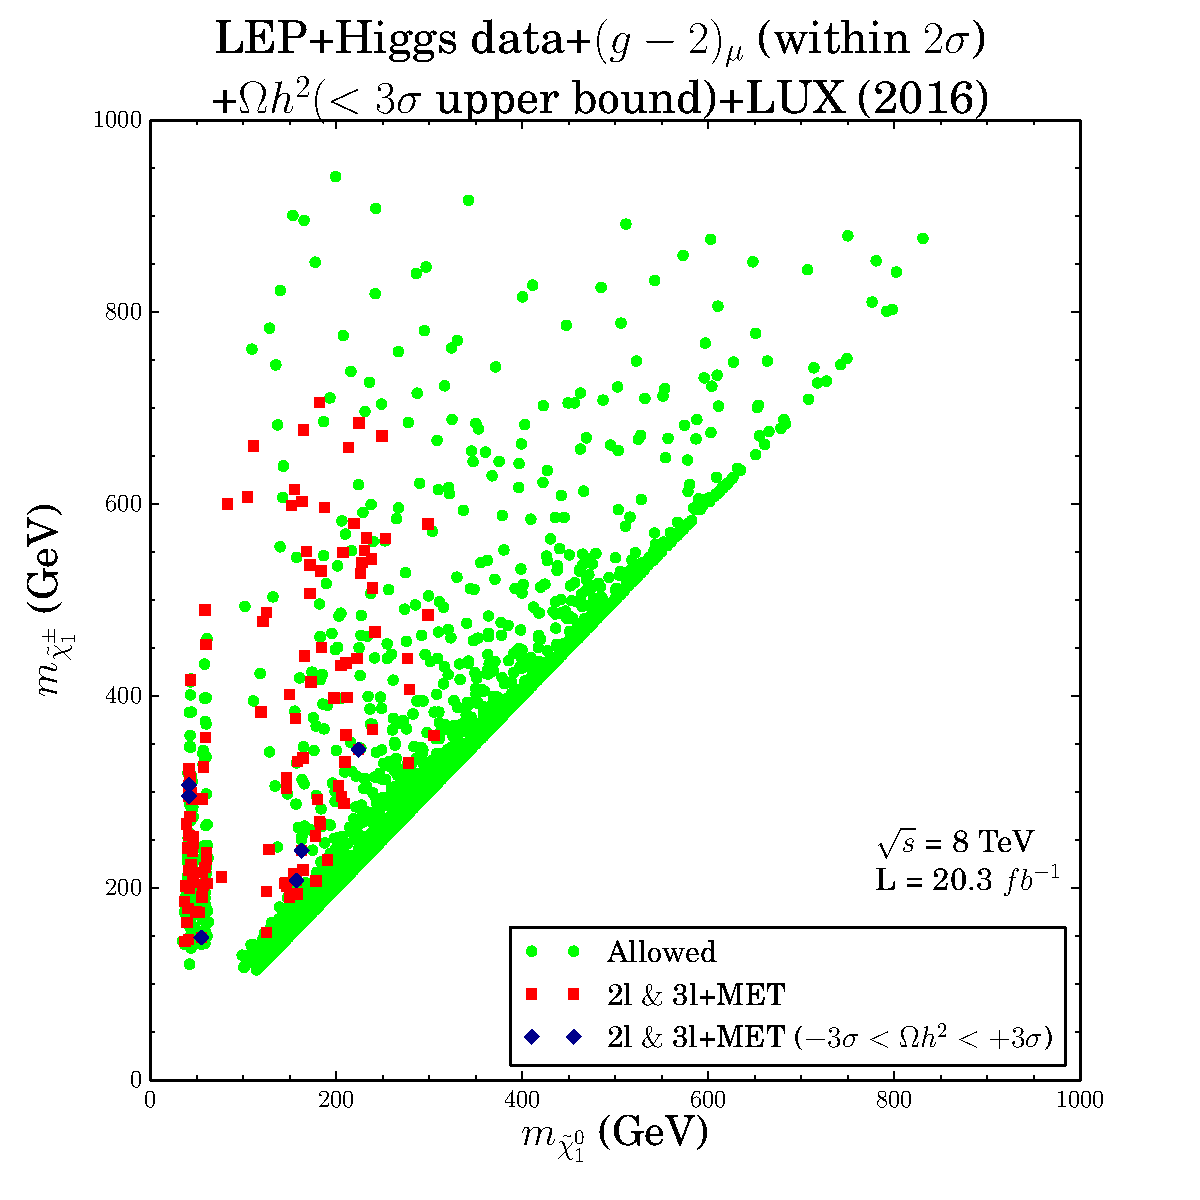
\includegraphics[scale=0.5]{figures/plot8TeV.png}
\captionof{figure}[Exclusion limits from $2\ell+\slashed{E}_T$ \& $3\ell+\slashed{E}_T$ events at $\sqrt{s}=8$ TeV LHC.]{Exclusion limits in the $m_{\tilde{\chi}^{\pm}_1} - m_{\tilde{\chi}^{0}_1}$ plane from LHC Run-I at $\sqrt{s}=8$ TeV from combined dilepton and trilepton events. All samples in the plot satisy LEP and Higgs constraints, $\Delta a_{\mu}$ within $2\sigma$ and the $3\sigma$ upper bound on the relic density as well as the LUX 2016 spin-independent cross-section 95\% C.L. exclusion limits. We sort the excluded $2\ell+\slashed{E}_T$ \& $3\ell+\slashed{E}_T$ samples into $\Omega h^2<+3\sigma$ (red squares) and $-3\sigma <\Omega h^2<+3\sigma$ (blue diamonds) where $\Omega h^2 \equiv \Omega_{DM} h^2 - \Omega_{Planck} h^2$.}
\label{fig:8Tevplot}
\end{center}

In Figure \ref{fig:8Tevplot}, we recast the exclusion limits coming from the LHC 8-TeV dilepton and trilepton searches, shown in the $m_{\tilde{\chi}^{\pm}_1} - m_{\tilde{\chi}^{0}_1}$ plane. All the samples present satisfy $\Delta a_{\mu}$ within $2\sigma$ as well as the LEP, Higgs and other collider constraints. They also satisfy the $3\sigma$ upper bound on the DM relic density and direct detection limits from LUX 2016. We further classify these into the dilepton and trilepton excluded points (blue diamonds), and a subset of these that satisfy both the upper and lower bound on the relic density (red squares). There is a portion of samples that can be excluded by the 8 TeV limits, namely for $\tilde{\chi}^{0}_1<300$ GeV and $\tilde{\chi}^{\pm}_1<710$ GeV. There is a significant number of samples that are not excluded lying around the region where $\tilde{\chi}^{\pm}_1$ and $\tilde{\chi}^{0}_1$ are almost degenerate. These are wino or Higgsino-like neutralino candidates. Scenarios like these are usually referred to as \textit{compressed spectra} since there is a small mass difference, $\Delta m$, between the LSP and the NLSP \cite{RN186}. Typically the soft decay products are difficult to access at the LHC, but can be probed using monojet-like signals to boost the initial state pair and enhance the missing $E_T$ of the final state. It has also been suggested in the Higgsino case to search for soft dileptons complementary to the monojet signal to boost the signal-to-background ratio rather than monojets alone which suffer from large SM background \cite{RN902,RN901,RN900}. Similarly, the small electroweak production rate can be studied in the context of Vector Boson Fusion (\acrshort{vbf}) production at LHC \cite{RN644}. The strategy for these analyses is to search for two forward opposite-hemisphere jets with large dijet invariant mass. Such analyses have been investigated in the context of the HL-LHC \cite{RN186,RN309,RN187,RN188,RN189,RN190,RN191}.
  
However, when the bino component of $\tilde{\chi}^0_2$ becomes dominant, the cross-section from $\tilde{\chi}^{\pm}_1 \tilde{\chi}^0_2$ becomes suppressed. In this case we find that the dilepton searches may become complimentary to the trilepton channel. The factor in determining this is the neutralino-leptonic branching fraction which can be quite sensitive to the configuration of the parameter space. We identify a number of cases:
\begin{enumerate}[label=(\alph*)]
\item When the slepton is on shell, the chargino two-body decay dominates with the leptonic branching fraction given by $\mathcal{B}(\tilde{\chi}^{\pm}_1 \rightarrow \nu_{\ell} \tilde{\ell}^{\pm} (\rightarrow \tilde{\chi}^0_1 \ell^{\pm}))_{\text{max}}=2/3$.
\item When the sneutrino is on-	shell and lighter than the corresponding slepton, the dominant decay mode will be $\tilde{\chi}^0_2 \rightarrow \nu_{\ell} \tilde{\nu_{\ell}}$ with the neutralino leptonic branching fraction suppressed.
\item When the sleptons and sneutrinos are heavy, the decay paths of $\tilde{\chi}^{\pm}_1$ and $\tilde{\chi}^0_2$ are dominated by $W$ and $Z$ decays, respectively. The branching fractions are given by $\mathcal{B}(\tilde{\chi}^{\pm}_1 \rightarrow \tilde{\chi}^0_1 W^{\pm} (\rightarrow \ell^{\pm} \nu_{\ell})) \simeq 2/9$ and $\mathcal{B}(\tilde{\chi}^0_2 \rightarrow \tilde{\chi}^0_1 Z (\rightarrow \ell^{\pm} \ell^{\mp})) \sim 6\%$, respectively. Otherwise if the decay path $\tilde{\chi}^0_1 \rightarrow h \tilde{\chi}^0_1$ is kinematically accessible, then the trilepton exclusion limits can be weakened  in this way.
\end{enumerate}

\section{Prospects for searches at a 100 TeV collider}

The frontier of particle physics hinges on the ability to resolve smaller and smaller distances (higher and higher energy scales) at colliders in order to probe fundamental new physics. In recent years, there have been proposals for a 100 TeV $pp$ collider that could potentially probe an order of magnitude energy scale higher than the LHC \cite{RN619} with promising prospects for detection of charged and neutral SUSY states \cite{RN194,RN195}. The integrated luminosity of such a machine may be as high as 3 ab$^{-1}$, the same as the target luminosity for the \acrshort{hllhc} upgrade, as we will use in this study.

In this section, we study the potential for a 100 TeV $pp$ collider to explain $\Delta a_{\mu}$ and the previous direct search constraints as well as those from DM relic density and LUX 2016. We extrapolate the allowed sample results from the 8 TeV search in the previous section using the most sensitive signal region. In this way, we simply rescale the signal $(S)$ and background $(B)$ events by the following ratio using the corresponding production cross-sections:
\begin{equation}
N^{100\,\text{TeV}}/N^{8\,\text{TeV}}=(\sigma^{100\,\text{TeV}}/\sigma^{8\,\text{TeV}})(\mathcal{L}^{100\,\text{TeV}}/\mathcal{L}^{8\,\text{TeV}}),
\end{equation}
where we have used the luminosities $\mathcal{L}^{8\,\text{TeV}}=20.3\,\text{fb}^{-1}$ and $\mathcal{L}^{100\,\text{TeV}}=3000\,\text{fb}^{-1}$. We consider such a treatment a preliminary theoretical estimate. Optimization of this strategy could be performed once the details of the collider environment become known. The expected signal exclusion criteria for the most sensitive signal region is taken as
\begin{equation}
\frac{S}{\sqrt{B+(\beta_{sys.}B)^2}} \geq 2 \qquad \text{[Excluded]},
\end{equation}
where the dimensionless factor $\beta_{sys.}$ parameterizes the systematic uncertainties. Figure \ref{fig:100Tevplot} shows the expected exclusion limits, where we can see that for $\beta_{sys.}=0.1$ we can probe a number of samples within $\tilde{\chi}^0_1 < 530$ GeV and $\tilde{\chi}^{\pm}_1 < 940$ GeV. This extends to $\tilde{\chi}^0_1 < 710$ GeV and $\tilde{\chi}^{\pm}_1 < 940$ GeV in the case where $\beta_{sys.}=0$.

We note that regions satisfying the relic density within the $3\sigma$ (upper and lower) range, through resonant annihilation in the `blind spot' region can now be searched for through the associated production process $\tilde{\chi}^0_2 \tilde{\chi}^+_1$ at the 100 TeV $pp$ collider. However, there are still samples outside the reach of future searches for trilepton events, corresponding to Higgsino/wino-like LSPs in the compressed mass spectrum region or bino-like LSPs that co-annihilate with the sleptons. The former may be probed through the monojet(-like) analysis at a future 100 TeV $pp$ collider, as explored in \cite{RN196}.

\begin{center}
	\includegraphics[scale=0.5]{figures/plot100TeV.png}
	\captionof{figure}[Exclusion limits from $2\ell+\slashed{E}_T$ \& $3\ell+\slashed{E}_T$ events at $\sqrt{s}=100$ TeV.]{Same as for Figure \ref{fig:8Tevplot}, but for $\sqrt{s}=100$ TeV and 3000 fb$^{-1}$ of data. Excluded $2\ell+\slashed{E}_T$ \& $3\ell+\slashed{E}_T$ samples are shown for the ranges $\Omega h^2<+3\sigma$ (red squares) and $-3\sigma <\Omega h^2<+3\sigma$ (blue diamonds) where $\Omega h^2 \equiv \Omega_{DM} h^2 - \Omega_{Planck} h^2$. The two figures correspond to $\beta_{sys.}=0.1$ and $\beta_{sys.}=0$, respectively.}
	\label{fig:100Tevplot}
\end{center}

\section{Concluding remarks}

This chapter has combined results from current and future $pp$ coliider and dark matter direct detection experiments to produce limits on the spectrum of electroweak sparticles that satisfy the anomalous magnetic moment of the muon, or $(g-2)_{\mu}$, in the MSSM. With all relevant constraints from Higgs and SUSY searches at LEP and LHC, measurements of the dark matter relic density from Planck and the PANDAX-II/LUX-2016 direct detection experiments, parts of the MSSM parameter space satisfying the $(g-2)_{\mu}$ can be significantly excluded. These limits could be further improved using the recent XENON-1T \cite{RN606,RN770} dark matter constraints and monojet searches \cite{RN196} at the LHC, especially for regions where the mass difference between the LSP and NLSP is small. In a broader context, our naive estimates in Figure \ref{fig:100Tevplot} give further motivation towards direct SUSY searches that shed light on low-energy observables like the $(g-2)_{\mu}$, and furthermore the development of next-generation colliders. It could be argued from these results that after the full run of next generation $pp$ colliders, one could finally close the lid on the simplest versions of supersymmetry satisfying the $(g-2)_{\mu}$ that simultaneously explain all (or part of) the dark matter abundance in the universe.

To close this chapter, we would also like to stress that despite the microscopic properties of the dark matter, the abundance significantly depends on its cosmological evolution of the early universe. More specifically, particular regions of excluded parameter space (i.e. predominantly bino-like LSPs) can actually become consistent with observation through depopulation mechanisms of cosmological origin, which are described in more detail in chapter \ref{chap:wimpdecay}.

  \chapter{Naturalness and fine-tuning beyond the MSSM}
\label{chap:finetuning}

\chapterquote{God used beautiful mathematics in creating the world.}%
{Paul Dirac, 1902--1984}

\noindent
The null results of supersymmetry at the CMS and ATLAS collaborations have put great constraint on the masses of coloured sparticles such as the gluino and squarks, leading to 95\% C.L. exclusion limits (within certain simplifying assumptions) of about $m_{\tilde{g}} \gtrsim 1.5$ TeV for $m_{\tilde{g}} \simeq m_{\tilde{q}}$ and $m_{\tilde{g}} \gtrsim 1$ TeV for $m_{\tilde{g}} \ll m_{\tilde{q}}$ \cite{RN567,RN568,RN569,RN693,RN695}. Recent $\sqrt{s}=13$ TeV results may suggest even stronger limits, excluding up to $\sim 2$ TeV gluinos and $\sim 1.5$ TeV squarks \cite{RN697,RN698}. It is particularly these limits that have hinted at the fact that the `natural' MSSM may not be realistic. Furthermore, it has been shown that in order to keep the MSSM `natural', one must keep the sparticle masses quite below the TeV scale \cite{RN699,RN239,RN700,RN701,RN703,RN702,RN704,RN705,RN706,RN707,RN708,RN710,RN709,RN711,RN712,RN713,RN714,RN715,RN716,RN717,RN719,RN720,RN721,RN722,RN691,RN723,RN724,RN69,RN5,RN253}.
\begin{center}
\includegraphics[scale=0.35]{figures/ATLAS_SUSY_Stop_tLSP.pdf}
\includegraphics[scale=0.35,trim={0 0.85cm 0 0},clip]{figures/ATLAS_SUSY_Strong_all.pdf}
\captionof{figure}[Limits on stops and gluinos.]{(Left) A Summary of the dedicated searches for stop pair production from ATLAS 3.2-36 $\text{fb}^{-1}$ data at $\sqrt{s}=13$ TeV, showing the 95\% C.L. exclusion limits in the $m_{\tilde{t}_1}-m_{\tilde{\chi}^0_1}$ plane. (Right) Exclusion limits at 95\% C.L. in the $m_{\tilde{g}}-m_{\tilde{\chi}^0_1}$ plane from ATLAS $\sqrt{s}=13$ TeV data for various simplified models of gluino decaying to the lightest neutralino \cite{RN695}.}
\label{fig:SUSYlimits}
\end{center}
Many of these models at large, however, come with a number of parameter relations usually as a result from some enhanced symmetries at the high-scale. Some studies have shown that this can lead to a significant reduction in fine-tuning. For example in \cite{RN716,RN712,RN749,RN750,RN751,RN752} one finds the existence of the `gaugino focus point' corresponding to a particular hierarchy of gaugino masses at the GUT scale. This could result from the embedding of SUSY in a larger gauge group structure or even from string theory. Similarly, the low-energy spectrum may contain degeneracies in the scalar masses coming from soft SUSY breaking stemming from cancellations between the tree and loop corrections to the Higgs boson mass leading to an overall reduction in fine-tuning (the so-called `focus-point') \cite{RN90,RN704,RN753,RN754,RN755}. Although as attractive as these prospects are, we in fact have no knowledge of the UV-complete supersymmetric Standard Model, or at which energy scale this should appear. More specifically, the failure for the MSSM to remain natural seems to hint that there is physics beyond the MSSM - whatever that may be. We have already mentioned the case where certain boundary conditions at the high scale can lead to reduction in fine-tuning - however one can also consider modifications to the Renormalization Group (RG) running down to low energies.

In this section, within the framework of this effective field theory, we parameterize our ignorance of the UV-physics and consider arbitrary variation in the 20-dimensional MSSM parameter space, for differing values of the unknown new physics intermediate scales $\Lambda$ in the next section. 

 Firstly, let us consider the minimization of the tree-level MSSM potential, which gives the following condition on the mass of the $Z$-boson:
\begin{equation}
\frac{m^2_Z}{2}=\frac{m^2_{H_d}-m^2_{H_u}\tan^2\beta}{\tan^2\beta-1}-|\mu|^2 \simeq -m^2_{H_u}-|\mu|^2,
\label{eqn:mZmincond}
\end{equation}
where the far right-hand side is valid for medium-to-large values of $\tan \beta$, or when $|m_{H_d}| \lesssim |m_{H_u}|$ for $\tan \beta \gtrsim 3$. For the one-loop MSSM Coleman-Weinberg potential \cite{RN684,RN683}, one simply makes the replacements
\begin{equation}
m^2_{H_u} \rightarrow m^2_{H_u} + \Sigma^u_u, \qquad  m^2_{H_d} \rightarrow m^2_{H_d} + \Sigma^d_d,
\end{equation}
where $\Sigma^u_u$ and $\Sigma^d_d$ are the one-loop corrections which include contributions from particles and sparticles with sizable Higgs-Yukawa or gauge-Higgs couplings. Eq. \ref{eqn:mZmincond} highlights a very important feature of the MSSM. This condition intrinsically connects the SUSY breaking scale, coming from the Higgs mass terms, with the electroweak breaking scale. In fact, since the $\mu$ term sets the masses of the Higgsinos in the MSSM, natural SUSY usually requires that the Higgsinos not exceed a couple hundred GeV \cite{RN685, RN686, RN684, RN687, RN688, RN689, RN690, RN691}. As is typically the case, the soft-SUSY breaking mass for the up-type Higgs doublet, $m_{H_u}$, is usually driven to negative values at the electroweak scale, triggering EWSB.

Hence, it is clear from the last equality in Eq. \ref{eqn:mZmincond} that we must adjust the low-energy values of $m_{H_u}$ and $\mu$ in such a way to reproduce $m_Z \simeq 91$ GeV. This can be achieved in a `natural' way when these adjustments are not sensitive to the variation in the fundamental parameters of the theory defined at some high scale, $\Lambda$. Quantitatively measuring this sensitivity, we invoke the standard Barbieri-Guidice measure \cite{RN239}:
\begin{equation}
\Delta = \max \left\{\left| \frac{a_i}{m^2_Z}\frac{\partial m^2_Z}{\partial a_i} \right| \right \},
\label{eqn:BGmeasure}
\end{equation}
where the $a_i$ are the fundamental parameters of the low-energy effective MSSM theory. These are of course renormalized through the RGEs down to the SUSY scale $M_{SUSY}$ at which the fine-tuning is actually evaluated. The quantity $\Delta$ represents the degree to which one must tune the independent parameters to correctly reproduce the electroweak scale. The application of the measure in the curly brackets in Eq. \ref{eqn:BGmeasure} to the right-hand side of Eq. \ref{eqn:mZmincond} results in
\begin{equation}
\frac{a_i}{m^2_Z}\frac{\partial m^2_Z}{\partial a_i}=\frac{2 a^2_i}{m^2_Z}\left( -\frac{\partial \mu^2}{\partial a^2_i} -\frac{\partial m^2_{H_u}}{\partial a^2_i} \right).
\end{equation}
Naively, one can estimate this fine-tuning at tree-level from $a_i=\{\mu^2,m^2_{H_u}\}$. We find
\begin{equation}
\Delta_{\mu} = -\frac{2\mu^2}{m^2_Z},\qquad \Delta_{m^2_{H_u}} = -\frac{2 m^2_{H_u}}{m^2_Z}.
\end{equation}
Again this tree-level analysis shows that in order to achieve low fine-tuning, one must have the absolute values of $\mu$ and $m^2_{H_u}$ at the electroweak scale to be comparable to the mass of the $Z$-boson.

Another question we may ask is: how much fine-tuning is actually acceptable? Of course this may differ among phenomenologists, however it is reasonable to accept that a value of $\Delta$ greater than 100 ($\Delta^{-1} \sim 1\%$ - corresponding to cancellations no more than 2 orders of magnitude) would amount to a fine-tuned theory. 

We approach the problem of fine-tuning in two ways. Firstly, we assume that the UV physics beyond the MSSM enters at a low enough scale such that the RG running of the ``fundamental" parameters is not strong enough to destabilize the electroweak minimum relationship in Eq. \ref{eqn:mZmincond}. Secondly, we look for relationships among parameters in the RGEs that correspond to infrared fixed-point behavior - implying that the values of the parameters satisfying the electroweak minimum condition are not particularly sensitive to their values at the input scale. We explore this case in sections \ref{sec:QFPMSSM} and \ref{sec:QFPscan}.

\section{General MSSM parameter scan}
\label{sec:generalscan}

Here we present our results for a general parameter scan over the 20-dimensional MSSM parameter space. We take a random sampling of the following parameter ranges:
\begin{eqnarray}
-3000\,\text{GeV} <& M_1,M_2 &< 3000\,\text{GeV}, \nonumber \\
&M_3 &< 3000\,\text{GeV}, \nonumber \\
-(3000)^2\,\text{GeV}^2 <& m^2_{H_u},m^2_{H_d} &< (3000)^2\,\text{GeV}^2, \nonumber \\
& m^2_{i_{1,2}} &< (3000)^2\,\text{GeV}^2, \nonumber \\
& m^2_{i_3} &< (3000)^2\,\text{GeV}^2, \nonumber \\
-3000\,\text{GeV} <& A_t,A_b,A_{\tau} &< 3000\,\text{GeV}, \nonumber \\
1 <& \tan \beta &< 50, \nonumber \\
&sign(\mu)&=\pm 1.
\label{eqn:param2}
\end{eqnarray}
where $i=(Q,\bar{u},\bar{d},L,\bar{e})$. Note that the first and second generation scalar soft masses are taken to be degenerate and similarly we assume no flavour mixing at the input scale (i.e. these are the diagonal entries of the matrices, we assume the off-diagonal entries are zero). In contrast to the philosophy adopted in chapter \ref{chap:muong-2}, and in virtue of the discussion in the previous section, we obviously cannot invoke decoupling of the third-generation squarks or gluino which are the main culprits in MSSM fine-tuning. However, the subsequent results in this chapter suggest that such a heavy spectra in the order of a few TeVs may indeed still remain natural pertaining to the important boundary conditions that we specify.

Eqs. \ref{eqn:param2} are the fundamental parameters of the theory entered at the following representative values of $\Lambda$:
\begin{equation}
\Lambda \in \left[10^5,10^{10},10^{16} \right]\,\text{GeV}.
\end{equation}
We employ the full two-loop RGEs using \texttt{SPHENO-3.3.8} \cite{RN178} combined with \texttt{SARAH} \cite{RN310} to compute both the MSSM spectrum and the fine-tuning measure. The parameters included in the calculation of the fine-tuning measure in Eq. \ref{eqn:BGmeasure} are the gaugino masses $M_1,M_2,M_3$, Higgs soft-breaking masses $m^2_{H_u},m^2_{H_d}$, 3rd generation scalar masses $m^2_{Q_3},m^2_{\bar{u}_3},m^2_{\bar{d}_3},m^2_{L_3},m^2_{\bar{e}_3}$, the trilinear couplings $A_t,A_b,A_{\tau}$, and the terms $\mu$ and $B_{\mu}$, all computed at the corresponding scale $\Lambda$. The top (pole) mass is set to 173 GeV. We also compute the DM relic density $\Omega_{DM} h^2$ and spin-independent WIMP-nucleon cross-section assuming a neutralino DM candidate using \texttt{micrOmegas-4.3.2} \cite{RN621}.

Points which have a vacuum in the electroweak broken phase are chosen which also satisfy $\Delta \leq 1000$ are subsequently passed through the following constraints:
\begin{itemize}
	\item Direct searches for the slepton and chargino at LEP produce the mass limits on the first two generation sleptons and lightest chargino \cite{RN493}:
	\begin{eqnarray}
	m_{\widetilde{l}_L},m_{\widetilde{l}_R} &>& 100\,\text{GeV}, \qquad (l=e,\mu), \\
	m_{\widetilde{\chi}^{\pm}_1} &>& 105\,\text{GeV},
	\end{eqnarray}
    \item We require the lightest Higgs boson mass in the range $122 < m_h < 128\,\text{GeV}$ \cite{RN62,RN63},
    \item We require the lightest neutralino $\widetilde{\chi}^0_1$ as the LSP and $m_{\widetilde{\chi}_1^0}>30\,\text{GeV}$ to be consistent with the bound on light MSSM neutralino dark matter \cite{RN232,RN775},
    \item We satisfy the 3 sigma upper bound on dark matter relic density observed by the Planck collaboration given by $\Omega_{Planck}h^2 = 0.112 \pm 0.006$ \cite{RN498}. For points with underabundant dark matter, we assume there may be some additional contribution from non-thermal candidates, such as the axion.
    \item We use the recent data from XENON1T \cite{RN606} to constrain the points with results from direct detection experiments, where we rescale the spin-independent cross-section $\sigma^{SI}$ to the observed relic density by $(\Omega_{DM} h^2/\Omega_{Planck}h^2)$,
    \item We check the bounds from Higgs searches at LEP, Tevatron and LHC implemented using \texttt{HiggsBounds-4.3.1} \cite{RN170},
    \item We also check important $B$-physics and flavour constraints, namely $\mathcal{B}(B\rightarrow X_s\gamma)$ and $\mathcal{B}(B_{S} \rightarrow \mu^{+}\mu^{-})$. The measured values we use are $\mathcal{B}(B\rightarrow X_s\gamma)_{\text{exp}}=(3.55 \pm 0.26)\times10^{-4}$ \cite{RN773} and the upper bound $\mathcal{B}(B_{S} \rightarrow \mu^{+}\mu^{-})_{\text{exp}}<1.08\times10^{-8}$ (95$\%$ CL) \cite{RN772}. These are calculated using \texttt{FlavorKit} \cite{RN771} as part of the \texttt{SPheno}/ \texttt{SARAH} package. Where an upper and lower bound are shown, we constrain our points to within $3\sigma$ of the quoted value.
\end{itemize}
We do not impose constraints from direct gluino/stop-squark searches from LHC as the limits are largely model-dependent and would require a dedicated recasting. Besides, there are many cases in which the spectrum may be compressed to easily avoid these LHC search constraints. In Figure \ref{fig:generalfine} we show the dependence on the fine-tuning measure on the gluino mass $M_{\tilde{g}}$ and lighter stop mass $M_{\tilde{t}_1}$.

\begin{center}
\includegraphics[scale=0.4]{figures/plot_mglu.png}
\includegraphics[scale=0.4]{figures/plot_mt1.png}
\captionof{figure}[Fine-tuning measure.]{Fine-tuning measure as a function of the gluino mass (top panel) and lighter stop mass (bottom panel) for three representative \acrshort{np} scales. Yellow squares contain LEP and Higgs mass constraints as well as $B$-Physics and Higgs precision constraints. The green squares are a subset of these containing DM relic density and direct detection constraints.}
\label{fig:generalfine}
\end{center}

Reductions in fine-tuning for the lower scales are indeed proportional to the amount of renormalization `running time', $\log \Lambda^2/m^2_Z$, and hence we see one can achieve a fine-tuning measure around $\mathcal{O}(10)$ for $\Lambda=100$ TeV. Furthermore, as we see in the plots in Figure \ref{fig:DMfine}, the dark matter constraints are satisfied relatively easily.

Since the electroweakino masses $M_1$ and $M_2$ enter the RGE for the up-type Higgs soft-breaking mass rather mildly (proportional to their respective gauge couplings), models with underabundant dark matter that are still compatible with direct detection constraints can exist without a strong contribution to the fine-tuning.

\begin{center}
	\includegraphics[height=0.21\paperheight]{figures/plot_nucleon.png}
	\includegraphics[height=0.21\paperheight]{figures/plot_relic.png}
	\captionof{figure}[Relic density and WIMP-nucleon spin-independent cross-section.]{Left: Relic density $\Omega_{DM}$ as a function of the LSP mass corresponding to the red squares in the rightmost panels of Figure \ref{fig:generalfine}. The dotted line corresponds to the PLANCK measurement of $\Omega_{Planck}h^2 = 0.112 \pm 0.006$ \cite{RN498}. Right: WIMP-nucleon spin-independent cross-section as a function of the LSP mass for the points shown in the left panel. Since we allow the LSP to be underabundant after freeze-out, we rescale the cross-section by the factor $\Omega/\Omega_{c}$ where $\Omega_{c}$ corresponds to the measured Planck Collaboration value. The solid lines corresponds to the XENON1T 2017 \cite{RN606} and the recent 1 tonne $\times$ year \cite{RN770} results. Similar plots exist for $\Lambda=10^{5}$ and $10^{10}$ GeV.}
	\label{fig:DMfine}
\end{center}

\section{The top-Yukawa infrared quasi fixed-point in the MSSM}
\label{sec:topqfp}

Consider the RGEs for the strong gauge coupling $g_3$ and the top-Yukawa coupling $y_t$ (given in appendix \ref{app:onelooprge}), in the absence of 2-loop or electroweak effects,
\begin{eqnarray}
\frac{dg_3}{dt}&=&-\frac{3g^2_3}{16\pi^2}, \\
\frac{dy_t}{dt}&=&\frac{y_t}{16\pi^2}\left( 6y^2_t - \frac{16}{3}g^2_3 \right),
\end{eqnarray}
where $t=\log (Q/Q_0)$ and $Q$ is the energy scale. One can easily verify that the ratio
\begin{equation}
\left(\frac{y^2_t}{g^2_3}\right)^{FP}=\frac{7}{18},
\end{equation}
is renormalization-invariant. This is the \textit{quasi-infrared fixed-point} (\acrshort{qfp}) \cite{RN747,RN748}, also known as the Pendleton-Ross fixed-point, since the top Yukawa coupling will track closer to the strong gauge coupling as one continues into the infrared. We show this behavior in Figure \ref{fig:topyuk}.

\begin{center}
\includegraphics[width=0.7\linewidth]{figures/TopYuk.png}
\captionof{figure}[Top-Yukawa quasi fixed-point behavior.]{The top Yukawa coupling $y_t$ expresses a quasi-infrared fixed-point evolving from $\Lambda=M_{GUT}$ to $m_Z$ at two-loop renormalization. Taken from \cite{RN746}.}
\label{fig:topyuk}
\end{center}

If one starts with a large top Yukawa coupling at a high scale, $\Lambda$ (could be the \acrshort{gut} scale), then we can even compute the value of $\tan \beta$ from the running top mass:
\begin{equation}
m_t(m_t)=\frac{y^{FP}_t v}{\sqrt{2}} \sin \beta,
\end{equation}
which of course is distinguishable from the physical top mass $m^{\text{pole}}_t$ which receives sizable one-loop corrections from (i) QCD gluons in the SM\footnote{This has the well-known result in the $\overline{DR}$ renormalization scheme \cite{RN741}:
\begin{equation}
\left(\frac{\Delta m_t}{m_t}\right)_{QCD}=\frac{5g^2_3}{12 \pi^2}.
\end{equation}}
and (ii) stops/gluinos from SUSY
\begin{equation}
m_t (m_t)= \frac{m^{\text{pole}}_t}{1 + \left(\frac{\Delta m_t}{m_t}\right)_{QCD} + \left(\frac{\Delta m_t}{m_t}\right)_{SUSY}},
\end{equation}
where the SUSY corrections are given by \cite{RN741,RN742,RN743,RN744,RN745}
\begin{eqnarray}
\left(\frac{\Delta m_t}{m_t}\right)_{SUSY}=-\frac{g^2_3}{12 \pi^2} \left\{ B_1 (m_t,m_{\tilde{g}},m_{\tilde{t}_1}) +B_1 (m_t,m_{\tilde{g}},m_{\tilde{t}_2}) \right. \\
\left. -\sin(2\theta_t)\frac{m_{\tilde{g}}}{m_t}\left[ B_0 (m_t,m_{\tilde{g}},m_{\tilde{t}_1}) -B_0 (m_t,m_{\tilde{g}},m_{\tilde{t}_2})\right] \right\},
\end{eqnarray}
where $\theta_t$ is the stop mixing angle and
\begin{equation}
B_n (p;m_1,m_2)=-\int^1_0 dx x^n \log \left[ \frac{(1-x)m^2_1+xm^2_2-x(1-x)p^2}{m^2_t}\right].
\end{equation}
Using the observed value for the top pole mass, this predicts a value for $\tan \beta$ of about 1.5 \cite{RN740}, which produces too light a Higgs boson mass at least at tree-level, requiring large stop-loop corrections (and/or stop mixing).

\section{Other QFPs in the MSSM and fine-tuning}
\label{sec:QFPMSSM}

Since the fixed-point property of $y_t$ has been well-known for a while, some studies have focused on the existence of quasi-fixed points for other couplings in the MSSM, such as the soft SUSY-breaking parameters when $y_t$ is in its quasi-fixed regime \cite{RN285,RN255,RN256,RN249,RN250,RN251}. In fact, it has been found that many of the soft SUSY-breaking masses have low-energy predictions independent of their high-scale input.

Our goal is to study the implications of these QFPs on the fine-tuning measure in the MSSM. In particular, because of the insensitivity of some of the low-energy parameters to their values at the high-scale, we would expect the fine-tuning measure to be significantly reduced in regions of QFP attraction.

Firstly, consider the one-loop RGE for the superpotential $\mu$ term
\begin{equation}
\frac{d}{dt}\mu=\frac{\mu}{16\pi^2}\left[3y^*_ty_t+3y^*_by_b+y^*_{\tau}y_{\tau}-3g^2_2-\frac{3}{5}g^2_1\right].
\end{equation}
where $t=\log(\Lambda^2/Q^2)$, where $Q$ is an arbitrary renormalization scale. Evidently, $\mu=0$ is a fixed-point of the theory, and moreover if $\mu$ is taken small at $\Lambda$ (say $\mu \sim m_Z$) then it shall stay small running to low energies (to all orders in perturbation theory). The evolution of $m^2_{H_u}$ with the energy scale is a little more involved, due to couplings to heavier particles in the spectrum:
\begin{equation}
\frac{d}{dt}m^2_{H_u}=\frac{1}{16\pi^2}\left[3X_t-6g^2_2|M_2|^2-\frac{6}{5}g^2_1|M_1|^2+\frac{3}{5}g^2_1S\right],
\label{eqn:mHubeta}
\end{equation}
where
\begin{equation}
S\equiv m^2_{H_u}-m^2_{H_d}+\text{Tr}[m^2_Q-m^2_L-2m^2_{\bar{u}}+m^2_{\bar{d}}+m^2_{\bar{e}}],
\end{equation}
and
\begin{equation}
X_t=2|y_t|^2(m^2_{H_u}+m^2_{Q_3}+m^2_{\bar{u}_3}+|A_t|^2).
\end{equation}
Since we know that $y_t$ is quasi-fixed in the infrared, a large $y_t$ at the high-scale enhances the initial contribution from $X_t$ at $\Lambda$, especially if $m^2_{H_u}$ is initially large. Similarly, if $M_1$ and $M_2$ are initially small, the remaining terms in Eq. \ref{eqn:mHubeta} are subdominant (they are also naturally suppressed by the square of the electroweak gauge couplings). We can write the RGE for $m^2_{H_u}$ in an approximate form:
\begin{equation}
\frac{d}{dt}m^2_{H_u}=\frac{6 y^2_t}{16\pi^2}m^2_{H_u}.
\label{eqn:mHubeta2}
\end{equation}
Similar to the $\mu$ parameter, this expresses a fixed point for $m^2_{H_u}=0$. From the observation in Eq. \ref{eqn:mHubeta2}, there is another important fixed-point we can see by defining the sum:
\begin{equation}
\Sigma=m^2_{H_u}+m^2_{Q_3}+m^2_{\bar{u}_3}+|A_t|^2,
\end{equation}
from which the beta function for $\Sigma$ satisfies:
\begin{equation}
\frac{d}{dt}\Sigma=\frac{3 y^2_t}{4\pi^2} \Sigma - \frac{2}{\pi^2}g_3^2 M^2_3.
\end{equation}
This clearly has a fixed point $\Sigma=0$ in the limit $M_3 \rightarrow 0$. However, due to the dynamics of $g_3$ and $M_3$, which increase in the infrared, we would expect a significant positive contribution to the evolution of $\Sigma$. In fact, this is evidence for the large fine-tuning present in a heavier spectrum. One finds for a positive $\Sigma$ at the weak scale, one must have a large (and negative) $m^2_{H_u}$ to cancel the 3rd generation squark masses $m^2_{Q_3}$ and $m^2_{\bar{u}_3}$. Similarly, since these parameters increase significantly in the infrared with large $y_t$, they can tend to destabilize $m^2_{H_u}$ very quickly. For this reason, we also consider the case of negative stop mass-squared values at the input scale\footnote{Negative stop mass-squared at the GUT scale, for example, can lead to a potential with a D-flat direction that is unbounded from below. This is improved with large loop corrections but can generate a large charge-colour breaking minimum which can be tunneled to by the EW minimum (if it has lower potential energy) \cite{RN778}. For the tunneling rate to be longer than the age of the universe (metastable), this leads to the following constraint on the running masses, $m_{\tilde{t}}(m_Z) \gtrsim \frac{1}{10}M_3 (m_Z)$ \cite{RN769}. This is easily satisfied in our scan.}. These have been studied previously in some gauge messenger models \cite{RN776} and also in the MSSM \cite{RN769,RN777} at the GUT scale. We show the evolution of $\Sigma$ and these soft-breaking masses in Figure \ref{fig:rgeplots}.

\section{Parameter scan in the quasi-fixed point region}
\label{sec:QFPscan}

In the following section we choose a large input top Yukawa coupling, $1 < y_t \lesssim \sqrt{4\pi}$, to enhance the running of $m^2_{H_u}$. This also requires the dominance of $m^2_{H_u}$ over the other scalar mass-squared parameters, most notably $m^2_{Q_3}$ and $m^2_{\bar{u}_3}$ individually. These will also tend to grow significantly with large $y_t$ into the infrared. Furthermore, the up-type Higgs soft-breaking mass parameter is also initially chosen to be large and negative, which is driven to small negative values at the weak scale, exploiting the quasi-fixed point behavior.

This scenario differs from the well-studied Radiative Electroweak Symmetry Breaking (\acrshort{rwesb}) mechanism \cite{RN563,RN903,RN904,RN905,RN907}, described as early as the 1980's, where the renormalization group equations drive $m^2_{H_u}$ to negative values at the weak scale, triggering electroweak symmetry breaking. An extraordinary property of this behavior is that the squarks and sleptons physical mass-squared can still remain positive. However, we also allow the stop masses to be tachyonic at the input scale, where their physical mass-squared values are driven positive at the weak scale. Although REWSB has the interesting property of naturally connecting electroweak symmetry breaking with SUSY breaking, we focus on a more unique set of boundary conditions in this framework. More precisely, we scan over the following modified parameter space:
\begin{center}
	\includegraphics[width=0.45\textwidth]{figures/sum100.png}
	\includegraphics[width=0.45\textwidth]{figures/rge100.png}
	\includegraphics[width=0.45\textwidth]{figures/sum1000.png}
	\includegraphics[width=0.45\textwidth]{figures/rge1000.png}
	\captionof{figure}[Quasi fixed-point behavior of the parameter $\Sigma$.]{Evolution of the parameter $\Sigma$ to the infrared fixed-point and soft mass parameters input at $\Lambda=10^{16}$ GeV with $m^2_{Q_3}=m^2_{\bar{u}_3}=-10^5\,\text{GeV}^2$, $A_t=-100$ GeV and $\tan \beta=10$. The three separate curves are shown for different initial values of: Top Row: $M_3=100\,\text{GeV},m^2_{H_u}=-10^5, -5\times 10^5, -10^6\, \text{GeV}^2$. Bottom Row: $M_3=1000\,\text{GeV},m^2_{H_u}=-5\times10^4, -10^5, -5\times10^5\, \text{GeV}^2$.}
	\label{fig:rgeplots}
\end{center}
\begin{eqnarray}
-3000\,\text{GeV} <& M_1,M_2 &< 3000\,\text{GeV}, \nonumber \\
&M_3 &< 3000\,\text{GeV}, \nonumber \\
-(3000)^2\,\text{GeV}^2 <& m^2_{H_u} &< 0, \nonumber \\
0 <& m^2_{H_d} &< (3000)^2\,\text{GeV}^2, \nonumber \\
0<& m^2_{i_{1,2}} &< (3000)^2 \,\text{GeV}^2, \nonumber \\
0<& m^2_{L_{3},\bar{e}_{3},\bar{d}_{3}} &< (3000)^2 \,\text{GeV}^2, \nonumber \\
-(1000)^2 \,\text{GeV}^2 <& m^2_{Q_{3},\bar{u}_{3}} &< (1000)^2 \,\text{GeV}^2, \nonumber \\
-3000\,\text{GeV} <& A_t,A_b,A_{\tau} &< 3000\,\text{GeV}, \nonumber \\
1 <& \tan \beta &< 50, \nonumber \\
&sign(\mu)&=\pm 1, \nonumber\\
1 <& y_t &< 3.
\end{eqnarray}
We also choose three representative high scales to enhance the running of $m^2_{H_u}$ through the top Yukawa coupling:
\begin{equation}
\Lambda \in \left[10^{10},10^{16},10^{19} \right]\,\text{GeV}.
\end{equation}
Again, satisfying the constraints detailed in section \ref{sec:generalscan}, we show the plots corresponding to the quasi-fixed point behavior in Figure \ref{fig:QFPplots}.
\begin{center}
	\includegraphics[scale=0.4]{figures/plot_mglu_QFP.png}
	\includegraphics[scale=0.4]{figures/plot_mt1_QFP.png}
\captionof{figure}[Fine-tuning measure in the quasi-fixed point regime.]{Same as in Figure \ref{fig:generalfine} with higher $\Lambda$ scales and in a narrower scan range supporting the infrared fixed-point behavior for $\Sigma$. Note the smaller y-axis range. Small fine tuning of $\Delta < O(100)$ can be achieved even for heavier sparticle masses $> 1$ TeV.}
\label{fig:QFPplots}
\end{center}
The plots shown in Figure \ref{fig:QFPplots} confirm our expectation showing significant reduction in fine-tuning in the quasi-fixed point regime, even holding at very high NP scales.

\section{Concluding remarks}

Through our consideration of naturalness, and in light of current experimental limits from the LHC, we believe that this is hinting towards evidence for physics beyond the MSSM. In this way, the MSSM is treated as an effective theory all the way up to a scale $\Lambda$ with no a priori assumption on the origin of soft-breaking terms. This is alternative to the often used boundary conditions assuming common scalar or gauginos at the GUT scale, for example. For our definition for acceptable fine-tuning, we observe the comfortable accommodation of multi-TeV coloured sparticles when the scale of new physics is even as low as $\Lambda = 10^{10}$ GeV and most certainly for $\Lambda = 100$ TeV. More precisely, we see the reduction of fine tuning from $\Delta \sim \mathcal{O}(100)$ for $\Lambda = 10^{16}$ GeV to $\Delta \sim \mathcal{O}(10)$ for $\Lambda = 10^5$ GeV in this case. But perhaps of greater interest is the existence of low-fine tuning ($\Delta < \mathcal{O}(100)$) when the MSSM behaves close to a quasi-fixed regime where the dynamics of the soft-breaking parameter $m^2_{H_u}$ becomes less sensitive to its value at $\Lambda$. Because of the importance of the gluino mass $M_3$ in the evolution of $m^2_{H_u}$ to low-energies, we find an upper limit of about $\sim$1.5 TeV on the gluino satisfying this naturalness criteria (and all other relevant constraints) when input at around the GUT scale and above. These results are of course indicative only - one could always perform a dedicated collider recasting outside the scope of our study. Nonetheless, this calls for a further exploration into non-standard UV completions to the MSSM.


  \chapter{A cosmological mechanism for depopulating dark matter}
\label{chap:wimpdecay}

\chapterquote{In order to make an apple pie from scratch, you must first create the universe.}%
{Carl Sagan, 1934--1996}

One of the notable concerns with neutralino dark matter in the MSSM is the familiar bino-like overabundance at early times, due to feeble annihilation rates. In this chapter, we describe a cosmological mechanism for reducing the abundance substantially through temporary decays. These early decays can arise from a spontaneously broken symmetry, which is then appropriately restored as the universe cools to stabilize the dark matter\footnote{An approach has been considered in \cite{RN739}, using additional auxiliary dark sector fields that require a specific mass arrangement.}.

In reference \cite{RN802} we discuss how this can be applied to a model of fermionic dark matter based on the inert \acrshort{2hdm} model \cite{RN602}, in which DM particles are odd under an imposed $Z_2$ symmetry and SM particles are even. In this case, at high temperatures the $Z_2$ symmetry is broken temporarily and then restored at lower temperatures, accounting for a phase in which the dark matter abundance is reduced through decays. Here instead we introduce a generic discussion of how we can exploit this mechanism in a model-independent fashion before exploring how this could be applied to the MSSM. In particular, dark matter in the MSSM can be destabilized in an analogous way through temporary $R$-Parity violation, a discrete $Z_2$ symmetry that prevents decay of the lightest neutralino to SM particles.

\section{A closer look at the WIMP relic density: The Boltzmann Equation}
\label{sec:boltzmann}

In the generic WIMP paradigm, dark matter particles were in thermal equilibrium with the constituents of the Universe in its early history. The departure from thermal equilibrium, where the dark matter decouples from the plasma occurs when the expansion rate of the Universe, $H$, overtakes the interaction rate of the heavy particles, $\Gamma$. We refer to this time in cosmological history as the WIMP \textit{freeze-out}, since the (co-moving) density of particles remains constant after decoupling - assuming it is kept stable (or is very long-lived compared to the age of the Universe) until the present day. If these particles were kept in equilibrium, they would have indeed been thermally suppressed by the factor $e^{-m/T}$. The Boltzmann equation for WIMP particles $\chi$ describing this process can be written as \footnote{Derivations of this equation in the form of Eq. \ref{eqn:boltzmann} can be readily found in \cite{RN785, RN682, RN681}.}:
\begin{equation}
a^{-3} \frac{d \left( n_{\chi} a^3\right)}{dt} = \left \langle \sigma v \right \rangle \left[ (n^{\text{EQ}}_{\chi})^2-n_{\chi}^2 \right].
\label{eqn:boltzmann}
\end{equation}
In the above, $a$ is the scale factor as usually defined through the Hubble expansion constant as $H \equiv \dot{a}/a$ and $n_{\chi}$ and $n^{\text{EQ}}_{\chi}$ are the dark matter number density and equilibrium number density, respectively. $\left \langle \sigma v \right \rangle$ is the thermally-averaged cross section, summed over all annihilation channels. It typically becomes convenient to factor out the effects of the universal expansion by using the number density of particles per co-moving volume. For this sake, let us then define the quantities
\begin{equation}
Y_{\chi} \equiv \frac{n_{\chi}}{s}, \qquad x \equiv \frac{m_\chi}{T}.
\end{equation}
$s=(2\pi^2/45)g_{*s}T^3$ is the entropy density, dominated by relativistic contributions, where
\begin{equation}
g_{*s}=\sum_{i=\text{bosons}} g_i \left( \frac{T_i}{T}\right)^3 + \frac{7}{8} \sum_{i=\text{fermions}} g_i \left( \frac{T_i}{T}\right)^3.
\end{equation}
In the early universe, at equilibrium, most species had identical temperatures, so $g_{*s}=g_*$. We will ignore dependence of $g_*$ on temperature, to good approximation. In general, the thermally-averaged cross section has dependence on velocity $v$, $\sigma v \propto v^p$ where $p=0$ is $s$-wave annihilation, $p=2$ is $p$-wave annihilation. Since $\left \langle v \right \rangle \sim T^{1/2}$, we parameterize the cross section as
\begin{equation}
\left \langle \sigma v \right \rangle \equiv \sigma_0 (T/m_{\chi})^n = \sigma_0 x^n,
\end{equation}
where $n=0$ corresponds to $s$-wave annihilation, $n=1$ for $p$-wave and so on. Changing from $t$ to the variable $x$, we require the Jacobian $dx/dt=Hx$. Hence, with all this we can write the Boltzmann equation for the abundance $Y_{\chi}$:
\begin{equation}
\frac{dY_{\chi}}{dx} = -\frac{\lambda}{x^{n+2}} \left[ Y_{\chi}^2-(Y^{\text{EQ}}_{\chi})^2 \right],
\label{eqn:YBoltz}
\end{equation}
where
\begin{equation}
\lambda = \left[ \frac{x s_{\chi} \left \langle \sigma v \right \rangle}{H_{\chi}}\right]_{x=1}.
\end{equation}
In the above, we have implied $s_{\chi}=(2\pi^2/45)g_{*}m^3_{\chi}$ and $H_{\chi}=(\pi^2g_{*}/90)^{1/2} (m^2_{\chi}/M_P)$ as the entropy density and Hubble expansion rate, respectively, both evaluated at $T=m_{\chi}$. For an $s$-wave process ($n=0$), $\lambda$ is constant, but in general higher partial waves mean that $\left \langle \sigma v \right \rangle$ may have some temperature dependence. We will ignore any temperature dependence on the thermally averaged cross-section. Similarly, it is safe for our purposes to ignore changes in $g_*$ with respect to temperature.

Initially, at $x \ll 1$, the relic abundance $Y_{\chi}$ approximately tracks the equilibrium abundance $Y^{\text{EQ}}_{\chi}$, which we can write as $Y_{\chi}(x)=Y^{\text{EQ}}_{\chi}(x)+\delta \approx Y^{\text{EQ}}_{\chi}(x)$. These equilibrium abundances have the simple forms:
\begin{eqnarray}
Y_{\chi}^{\text{EQ}}(x)=\left\lbrace
\begin{array}{ll}
\frac{45}{2\pi^4}\left(\frac{\pi}{8}\right)^{1/2}\frac{g_{\chi}}{g_{*}}x^{3/2}{e}^{-x}~, & m_{\chi} \gg T, \\
	\frac{45\zeta(3)}{2\pi^4}\frac{g_{\text{eff}}}{g_{*}} \simeq 0.278\frac{g_{\text{eff}}}{g_{*}}~, & T \gg m_{\chi}, \\ 
\end{array} 
\right.
\label{eqn:equilbabund}
\end{eqnarray}
where $g_{eff}=g_{\chi}$ $(g_{eff}=3g_{\chi}/4)$ measures the degrees of freedom for bosonic (fermionic) dark matter. For relativistic particles, clearly $Y_{\chi}^{\text{EQ}}$ remains constant up until the dark matter becomes relativistic (or $x>1$). For non-relativistic dark matter, $Y_{\chi}^{\text{EQ}}$ becomes exponentially suppressed at later times and the $Y_{\chi}$ will dominate completely. At this point, the dark matter scatterings are so rare that they cannot maintain equilibrium in the thermal bath. At close to freeze-out, the departure from equilibrium is significant and $Y_{\chi} \approx \delta \gg Y_{\chi}^{\text{EQ}}$ ($x \sim x_f$) where
\begin{equation}
\delta(x) \approx \frac{x^{n+2}}{2\lambda}.
\label{eqn:delta}
\end{equation}
For $x \gg x_f$ one can then drop the equilibrium yield from Eq. \ref{eqn:YBoltz} and integrate from the freeze-out to the present day, $x_{\infty}$ to give:
\begin{equation}
Y^{\infty}_{\chi} \approx \frac{(n+1)Y_{\chi}(x_f)x^{n+1}_f}{Y_{\chi}(x_f)\lambda + (n+1)x^{n+1}_f},
\label{eqn:Yxf}
\end{equation}
where $Y_{\chi}(x_f)=\delta(x_f)$ for non-relativistic dark matter. For relativistic dark matter at decoupling, $Y_{\chi}(x_f)=Y_{\chi}^{\text{EQ}}$. Typically, the correct relic abundance when the decoupling is non-relativistic occurs when $x_f \sim \mathcal{O}(10)$, and so in summary, the final yield of dark matter for these situations are:
\begin{eqnarray}
Y^{\infty}_{\chi}=\left\lbrace
\begin{array}{ll}
\frac{(n+1)x^{n+1}_f}{\lambda}~, & \text{non-relativistic} \\
0.278\,(0.208)\frac{g_{\text{eff}}}{g_{*}}~, & \text{relativistic bosons (fermions)} \\ 
\end{array} 
\right.
\label{eqn:Ychiinf}
\end{eqnarray}
Since we typically have $\lambda \gg 1$, the relativistic decoupled dark matter is several orders of magnitude higher than the non-relativistic decoupling. This is finally recast into the form of the fraction of present-day critical density from $\chi$,
\begin{equation}
\Omega_{\chi} = \frac{m_{\chi}Y^{\infty}_{\chi} s_0}{3 H^2_0 M^2_P},
\end{equation}
where $s_0=2891.2\,\text{cm}^{-3}$ and $H_0=100\,h\,\text{km}\, \text{s}^{-1}\,\text{Mpc}^{-1}$ $(h=0.673)$ are the present day entropy density and Hubble expansion rate \cite{RN493}.

\begin{center}
\includegraphics[width=0.6\linewidth]{figures/KolbTurner.jpg}
\captionof{figure}[WIMP freeze-out abundance.]{The typical `freeze-out' description of a non-relativistic DM species from equilibrium with the surrounding plasma at about $x_f \sim \mathcal{O}(10)$. The dashed line shows the abundance of DM per comoving volume element, whilst the solid line is the equilibrium abundance. Adapted from \cite{RN681}.}
\label{fig:KolbTurner}
\end{center}

\section{Decays from a cosmological phase transition}
\label{sec:Decays}

Let us suppose that there is a symmetry stabilizing the DM up to a time $x_a$, in which this symmetry is spontaneously broken. This cosmological phase transition persists until $x_b$, in which the symmetry is then restored. Hence, during the instability phase $x \in [x_a , x_b]$, the DM is permitted to decay. As seen in the previous section, we would require that the dark matter be non-relativistic for some, if not all, of the instability phase in order to suppress inverse decays that would repopulate the dark matter. The Boltzmann equation in Eq. \ref{eqn:YBoltz} then gets modified with a decay term\footnote{In general, we should include the thermally-average decay width $\langle \Gamma_{\chi} \rangle= \Gamma_{\chi}K_1 (x)/K_2 (x)$ where $\Gamma_{\chi}$ is the zero-temperature width and $K_n(x)$ are the modified Bessel functions \cite{RN782,RN784,RN783}. For non-relativistic DM, this has the asymptotic form $K_1(x)/K_2(x)=1-3/(2x)+\mathcal{O}(x^{-2})\, (x \gg 1)$ and so can be approximated by the zero-temperature width, whilst for relativistic dark matter is $K_1(x)/K_2(x)=x/2+\mathcal{O}(x^2)\, (x \ll 1)$ (see Appendix \ref{app:specfunc}). Hence, we neglect DM decay before it becomes non-relativistic since they are highly suppressed.}:
\begin{equation}
	\frac{dY_{\chi}}{dx}=-\frac{2\Gamma_{\chi}x}{g_{\chi}H_{\chi}}\left[Y_{\chi}-Y_{\chi}^{\text{EQ}}\right]-\frac{\lambda}{x^{n+2}}\left[Y_{\chi}^2-\left(Y_{\chi}^{\text{EQ}}\right)^2\right]\;.
    \label{eqn:YBoltzDecay}
\end{equation} 
Here $\Gamma_{\chi}$ is the decay width of the DM particle.

Before we consider the effects of decays on dark matter density, we must first comment on the consequence of entropy production during the phase transition, which can also dilute the dark matter density when it is a first-order transition \cite{RN787,RN786}. Since the phase transition occurs well above $T=1$ GeV, we can neglect entropy production from particle decoupling, or in other words, we can assume $g_*$, the number of relativistic degrees of freedom, is approximately constant. The change in entropy can then be parameterized by a dilution factor (as in \cite{RN787}) where $\gamma \equiv s(x_f)/s(x_i)$ such that the final density changes as
\begin{equation}
	Y^{\infty}_{\chi} \rightarrow \frac{Y^{\infty}_{\chi}}{\gamma}, \quad \Omega_{\chi} \rightarrow \frac{\Omega_{\chi}}{\gamma},
\end{equation}
where $\gamma > 1$. Here, $x_i$ and $x_f$ represent the beginning and after the phase transition, respectively. This is valid for the case where the dark matter density is much larger compared to its equilibrium abundance, $Y_{\chi} \gg Y^{EQ}_{\chi}$, as is the case after freeze-out and annihilations are negligible compared to decays. However this also holds for DM yields that are close to their equilibrium value, $Y_{\chi} \sim Y^{EQ}_{\chi}$. In many general cases, the analytical solutions are not available.

The effect of the DM decays depends on when this instability takes place relative to the time of freeze-out, and the size of the decay rate $\Gamma_{\chi }$. Let us consider (4) separate scenarios:
\begin{enumerate}[label=(\arabic*)]
\item \textit{Freeze-out precedes first phase transition}, $x_f \ll x_a$. Here we expect a significant change in the final density of dark matter. In Eq. \ref{eqn:YBoltzDecay}, the equilibrium yield would be exponentially suppressed, which then resembles the Bernoulli equation and is analytically solvable in terms of the incomplete Gamma function, $\Gamma(\alpha,x)$:
\begin{align}
	Y_\chi(x_b) &= \frac{ Y_{\chi }(x_a)    e^{-\frac{\Gamma _{\chi }}{2 H_{\chi }} x_b^2}}{ e^{-\frac{\Gamma_{\chi}}{2 H_\chi}x_a^2}  + \lambda\, Y_\chi(x_a)\,\frac{1}{2} \left(\frac{\Gamma _{\chi }}{2 H_{\chi }}\right)^{\frac{n+1}{2}}
	\left[
		\Gamma \left(\frac{-1-n}{2},\frac{ \Gamma _{\chi }}{2 H_{\chi }} x_a^2\right)
 - \Gamma \left(\frac{-1-n}{2},\frac{ \Gamma _{\chi }}{2 H_{\chi }} x_b^2\right)
\right]}\\
&\approx
\frac{  Y_{\chi }(x_a)    e^{-\frac{\Gamma _{\chi }}{2 H_{\chi }} (x_b^2-x_a^2)}}{ 1 + \lambda\,Y_\chi(x_a) \,\frac{  H_\chi}{\Gamma_\chi} 
	\left[
		\frac{1}{x_a^{3+n}}
		-\frac{e^{-\frac{\Gamma_\chi}{2 H_\chi} (x_b^2-x_a^2)}}{x_b^{3+n}}
\right]}.
\label{eqn:Yxb1}
   \end{align}
The second line uses a leading-order asymptotic expansion for the incomplete Gamma function, for fixed $\alpha$ and large $x$ (this is detailed in appendix \ref{app:specfunc}). The scattering cross-section is present in Eq. \ref{eqn:Yxb1} through the matching condition, i.e. $\lambda Y_{\chi}(x_a) \approx (n+1)x_f^{n+1}$ for non-relativistic freeze-out at $x_f$. The exponential suppression factor $\Gamma_{\chi}(x^2_b - x^2_a)/H_{\chi}$ in Eq. \ref{eqn:Yxb1} has a simple intuitive explanation. The reduction of dark matter density is defined through the decay rate of dark matter per the universal expansion rate multiplied by the decay time $\Delta t \propto x^2_b - x^2_a$, or the duration of the phase transition. Finally, the present day abundance $Y^{\infty}_{\chi}$ can be obtained by substituting $Y_{\chi}(x_f) \rightarrow Y_{\chi}(x_b)$ into Eq. \ref{eqn:Yxf}.

\item \textit{Freeze-out occurs during instability phase}, $x_a < x_f < x_b$. In this case, we can solve Eq. \ref{eqn:YBoltzDecay} with the ansatz $Y_{\chi}=Y_{\chi}^{EQ} + \delta_d$, where $\delta_d$ parameterizes a small deviation from the equilibrium yield. Hence, we get the following solution for $x_a < x_f$:
\begin{equation}
\delta_d (x) \approx -\frac{dY_{\chi}^{EQ}}{dx}\left[\frac{\Gamma_{\chi}}{H_{\chi}}x+\frac{2\lambda}{x^{n+2}}	Y_{\chi}^{EQ} \right]^{-1},
\label{eqn:deltad}
\end{equation}
where we have neglected $\delta'_d$ and $\mathcal{O}(\delta_d^2)$ terms. For the period $x_a < x < x_f$, the solution is given by Eq. \ref{eqn:deltad}. For the subsequent period of $x_f < x < x_b$, if inverse decays are negligible, we can then implement the solution in Eq. \ref{eqn:Yxb1}, provided we match the solutions with $Y_{\chi}(x_a) \rightarrow Y_{\chi}(x_f) = Y^{EQ}_{\chi}(x_f)+\delta_d (x_f)$. Then the present-day abundance is simply given by $Y_{\chi}(x_f) \rightarrow Y^{EQ}_{\chi}(x_b)$ in Eq. \ref{eqn:Ychiinf}. Conversely, if the inverse decays are fast enough to keep the DM in equilibrium through the whole phase, we can use Eq. \ref{eqn:Ychiinf} to simply recast the final abundance as:
\begin{equation}
Y^{\infty}_{\chi} \approx \frac{(n+1)Y^{EQ}_{\chi}(x_b)x^{n+1}_b}{Y^{EQ}_{\chi}(x_b)\lambda + (n+1)x^{n+1}_b}.
\label{eqn:Yxbinf}
\end{equation}
We consider an explicit numerical example of this particular case in \cite{RN802}.
\item \textit{Freeze-out immediately follows second phase transition}, $x_f \sim x_b$. If the decay width $\Gamma_{\chi }$ is large enough its dominance will ensure $Y^{EQ}_{\chi}(x_f) \gg \delta_d (x_f)$ and decays will keep the DM abundance exponentially close to the equilibrium value at freeze-out. This is different of course to the case of pure scatterings. Consequently, one can then obtain the present day abundance through the substitution $Y_{\chi}(x_f) \rightarrow Y^{EQ}_{\chi}(x_f)$ in Eq. \ref{eqn:Ychiinf}, and may be substantially smaller than in Eq. \ref{eqn:Ychiinf}.

\item \textit{Freeze-out succeeds second phase transition}, $x_f \gg x_b$. In this case, the scatterings that would occur subsequently after the phase transition would re-populate the dark matter. This would lead to essentially the same abundance at freeze-out, given in Eq. \ref{eqn:Ychiinf}.
\end{enumerate}
For situations not considered here, it is always possible to solve Eq. \ref{eqn:YBoltzDecay} numerically to obtain the final yield.

\section{Regeneration and present-day abundance}
\label{sec:Regen}

During the phase of instability, $x \in [x_a,x_b]$, suppose we have a scalar which spontaneously breaks the symmetry responsible for stabilizing the DM. There may also be Goldstone modes or massive gauge bosons from the breaking of other continuous symmetries. These can be produced via decays of the DM particle and through scatterings with SM particles. Since the VEV of the $S$ degree of freedom increases as $v^2_s \propto 1-x^2_a/x^2$ in $x \in [x_a,x_b]$, these degrees of freedom may stay relativistic or could become non-relativistic depending on their thermal mass compared to the temperature up until and at $T_b$.

After the second phase transition, all degrees of freedom associated with $S$ are heavy and therefore follow the Maxwell-Boltzmann distribution. We first assume that all relativistic $S$ degrees of freedom are in kinetic and chemical equilibrium at some point during the instability phase, at least at the end leading up to $T_b$. Let us also assume that these scalars are still in kinetic equilibrium with the SM thermal bath after this phase transition such that they will have the same temperature, $T_b$. This is satisfied when the relaxation rate $\Gamma_{relax} \simeq \Gamma_{coll}/N_{coll}$ (where $\Gamma_{coll}$ is the collision rate and $N_{coll}$ is the number of collisions) exceeds the Hubble rate $H \lesssim \Gamma_{relax} \simeq \frac{T}{3m_S} \Gamma_{coll}$ which is a valid assumption\footnote{In general, we can fulfill this condition if we consider scalar interactions with electroweak bosons. The collision rate can then be estimated as $\Gamma_{coll} \simeq G^2_F T^5$ for non-relativistic $S$ scattering with a relativistic particle in the SM thermal bath. Kinetic equilibrium can then be achieved when $T^4 \gtrsim m_S/G^2_F M_P \simeq (40\,\text{MeV})^4(m_S/\text{TeV})$.} \cite{RN806,RN807}. Since the number density of initially relativistic particles also doesn't change after the symmetry-restoration at $x_b$, we can in general write
\begin{equation}
	\frac{\zeta(3)}{\pi^2}T^3_b = \left( \frac{m_S T_b}{2\pi}\right)^{3/2} e^{(\mu-m_S)/T_b} \Rightarrow \mu \approx m_S,
	\label{eqn:number1}
\end{equation}
where $\mu$ is the associated chemical potential. Since $\mu \sim m_S \gg T_b$ the scalar is initially over-abundant since $Y_S/Y^{EQ}_S \sim \exp(m_S/T_b)$. The particles which become non-relativistic during the instability phase will then follow a Maxwell-Boltzmann distribution during and after $x_b$. Since their mass may change after the phase transition, but still maintaining the same number density, we have
\begin{eqnarray}
	\left( \frac{m'_S T_b}{2\pi}\right)^{3/2} e^{-m'_S / T_b} &=& \left( \frac{m_S T_b}{2\pi}\right)^{3/2} e^{(\mu-m_S)/ T_b} \nonumber \\ &\Rightarrow& \mu \approx m_S - m'_S + \frac{3}{2} T_b \log (m'_S/m_S),
\end{eqnarray}
where $m'_S$ is the mass of the scalar after the instability phase and $m_S$ is the mass at zero temperature. Hence, the scalar $S$ can be overabundant, $Y_S/Y^{EQ}_S \sim (m'_S/m_S)^{3/2} \exp (m_S-m'_S)/T_b$ right after this phase transition, though closer to equilibrium compared to Eq. \ref{eqn:number1}.

Since the scalars are heavier than the mass of the DM, and are non-relativistic, they can annihilate to DM and an SM particle. This phase we call regeneration. Assuming that DM annihilations have become negligible, one can write the analogous Boltzmann equations for the regeneration phase:
\begin{eqnarray}
	\frac{dY_S}{dx} &=& -\frac{\Gamma_S x}{H_{\chi}} \left( Y_S - \frac{Y_{\chi}}{Y^{EQ}_{\chi}}Y^{EQ}_S\right) - \frac{\lambda_S}{x^{m+2}}\left( Y^2_S - (Y^{EQ}_S)^2\right), \\
	\frac{dY_{\chi}}{dx} &=& \frac{\Gamma_S x}{H_{\chi}} \left( Y_S - \frac{Y_{\chi}}{Y^{EQ}_{\chi}}Y^{EQ}_S\right),	
\end{eqnarray}
where $\Gamma_S$ is the zero-temperature decay width for the scalar, which is suitable since $S$ is non-relativistic. Likewise, we may write the annihilation cross-section for $S$ into SM fermion pairs as before:
\begin{equation}
\lambda_S = \left[ \frac{x s_{\chi} \left \langle \sigma v (SS \rightarrow f\bar{f})\right \rangle}{H_{\chi}}\right]_{x=1}.
\end{equation}
Here we have $m=0$ for $s$-wave scattering and $m=1$ for $p$-wave. However, we again approximate the thermally-averaged cross-section by the leading partial wave.

We briefly summarize the relevant timescales in this regeneration phase: (i) the freeze-out of the scalar $S$, $x^S_f$, given by $H(x^S_f)=n_S \left \langle \sigma v (SS \rightarrow f\bar{f})\right \rangle_{x=x^S_f}$; (ii) the chemical equilibrium of $S$, $x^S_c$, where $Y_S (x^S_c)=Y^{EQ}_S (x^S_f)$; and (iii) when inverse decays become sizable, $x^S_i$, where $Y_S (x_i) Y^{EQ}_{\chi} (x_i) = Y_{\chi} (x_i) Y^{EQ}_S (x_i)$. The phenomenology changes significantly depending on how these are ordered. However, at the second phase transition, since we have $Y_S(x_b) \gg Y^{EQ}_S (x_b)$ and $Y_S$ decreases with $x$ such that $Y_S(x) \gg Y^{EQ}_S (x)$, in general we can conclude $x^S_i \leq x^S_c$.

In Figure \ref{fig:DMscenarios}, we present two separate scenarios that may be realized within this general framework.
\newpage
\begin{center}
	\includegraphics[width=0.45\linewidth]{figures/PlotDMDecay.png}
	\includegraphics[width=0.45\linewidth]{figures/PlotDMNum.png}
	\captionof{figure}[DM depopulation scenarios.]{Schematic illustrations of two distinct scenarios in the depopulation of thermal dark matter. (Left) This corresponds to (1) in section \ref{sec:Decays}, where the equilibruim yield is negligible at the beginning of the phase transition. In this case, inverse decays partially repopulate the dark matter after the second phase transition leading to the present day abundance.		
	(Right) This is the case described by (2) in section \ref{sec:Decays}. Since inverse decays are fast enough to keep the DM in equilibrium, the equilibrium abundance at the end of the phase transition, $Y^{EQ}_{\chi}(x_b)$, leads to the present day abundance of dark matter.}
	\label{fig:DMscenarios}
\end{center}

\section{Application to the MSSM \& $R$-Parity violation}
\label{sec:MSSMapp}
The multiple scalar states involved in supersymmetric theories makes them ideal models to study the depopulation mechanism. Moreover, we have seen that significant parts of the MSSM parameter space lead to bino-like DM candidates with relic abundances many orders larger than observation because of their feeble annihilation rate. Of course the neutralino DM candidate is stabilized by the discrete $R$-parity, but this can be temporarily broken (and of course stabilized in the zero-temperature limit) in the early universe, leading to an exponential decay period to reduce the abundance significantly. One way to accomplish this is through the condensation of the sneutrino, assuming all the other extra states of the MSSM remain heavy and decoupled. Using the Higgs boson tree-level mass in Eq. \ref{eqn:mhtree}, the zero temperature scalar potential in this particular limit is the following \cite{RN793}: 
\begin{equation}
V_0=-\frac{m_h^2}{4}h^2+m^2_{\tilde \nu}|\tilde \nu|^2+\frac{m_Z^2}{8v^2}\left(\frac{m_h}{m_Z}h^2+2|\tilde \nu|^2\right)^2~, \label{eqn:sneutrinopot}
\end{equation}
where $m_{\tilde \nu}$ here is the sneutrino soft SUSY breaking mass. We are interested in a phase where the sneutrino develops a non-zero vacuum expectation value, and hence we allow it to be tachyonic\footnote{This assumption is atypical, yet in some cases, phenomenologically viable. Tachyonic soft masses may emerge in some specific supersymmetry breaking scenarios at high energies. For example, the implications of a negative common scalar mass at the GUT scale in the context of minimal supergravity (\acrshort{msugra}) is discussed in \cite{RN768}.}. The physical sneutrino mass, however, receives contribution from the electroweak symmetry breaking and radiative corrections. The physical mass-squared, 
\begin{equation}
M_{\tilde \nu}^2=m_{\tilde \nu}^2+\left(\frac{m_Zm_h}{2} + \text{rad. corr.}\right),
\end{equation}
must obviously be positive, and therefore the following constraint must be met: 
\begin{equation}
-\left(\frac{m_Zm_h}{2} + \text{rad. corr.}\right)< m_{\tilde \nu}^2< 0.
\end{equation}

\subsection{Finite temperature corrections}
In the high-temperature limit, we have contributions to the effective potential from thermal loops. We will only consider contributions from $h$ and $\tilde{\nu}$, the electroweak gauge bosons and the top quark. We will neglect all the sub-dominant Yukawa couplings. The finite temperature contributions are given by
\begin{equation}
\Delta V^{(1)}(\phi_c,T)=\frac{T^4}{2\pi^2} \left[ \sum_{i} n_i J_B [m^2_i (\phi_c)/T^2] + n_t J_F [m^2_t (\phi_c)/T^2] \right],
\end{equation}
where $i=\left\{h,\tilde{\nu},W^{\pm},Z\right\}$ and $J_B$ and $J_F$ are the boson and fermion thermal functions, respectively, defined in the high-temperature limit as
\begin{eqnarray}
J_B(m/T)&=&-\frac{\pi^4}{45}+\frac{\pi^2}{12}\frac{m^2}{T^2}-\frac{\pi}{6}\left(\frac{m^2}{T^2} \right)^{3/2}-\frac{1}{32}\frac{m^4}{T^4}\log \frac{m^2}{a_b T^2}+\mathcal{O}\left( \frac{m^6}{T^6}\right), \\
J_F(m/T)&=&\frac{7\pi^4}{360}-\frac{\pi^2}{24}\frac{m^2}{T^2}-\frac{1}{32}\frac{m^4}{T^4}\log \frac{m^2}{a_f T^2}+\mathcal{O}\left( \frac{m^6}{T^6}\right),
\end{eqnarray}
where $a_b=16\pi^2 \exp (3/2-2\gamma_E)$ ($\log a_b = 5.4076$) and $a_f=\pi^2 \exp (3/2-2\gamma_E)$ ($\log a_f = 2.6351$). $\gamma_E \approx 0.5772$ is the Euler-Mascheroni constant. $m^2$ is the thermally \textit{shifted} mass, computed from the tree-level potential as:
\begin{equation}
m^2 (\phi_c) = \frac{d^2 V_0 (\phi_c)}{d\phi^2_c}.
\end{equation}
We show a more detailed derivation of the origin of the finite-temperature contributions to the potential in appendix \ref{app:thermcorr}. The $n_i$ represent the degrees of freedom of the $i$th species, which are
\begin{align}
&n_h=1, n_{\tilde{\nu}}=2, \\
&n_W=6, n_Z=3, n_t=-12.
\end{align}
Therefore, the thermal masses for the scalar boson species are:
\begin{eqnarray}
m^2_{h}(h,\tilde{\nu})& \simeq & -\frac{m^2_h}{2}+\frac{3m^2_h}{2v^2}h^2+\frac{m_z m_h}{v^2}|\tilde{\nu}|^2, \\
m^2_{\tilde{\nu}}(h,\tilde{\nu})& \simeq & m^2_{\tilde{\nu}}+\frac{m_z m_h}{v^2}h^2+\frac{6m^2_z}{v^2}|\tilde{\nu}|^2.
\end{eqnarray}
Similarly, the top-quark mass is defined through the Yukawa coupling, $y_t$. The dominant high temperature corrections to the potential in Eq. \ref{eqn:sneutrinopot} (ignoring linear and logarithmic terms in $T$) reads:
\begin{eqnarray}
V_T&=& \frac{\alpha_hT^2}{2}h^2+\alpha_{\tilde \nu}T^2|\tilde \nu|^2~, \\
\label{eqn:ah}
\alpha_h &=&\frac{1}{8v^2}\left(4m_W^2+2m_Z^2+4m_t^2+m_h^2+\frac{2}{3}m_Zm_h\right)\approx 0.383~, \\
\label{eqn:anu}
\alpha_{\tilde \nu} &=&\frac{1}{8v^2}\left(4m_W^2+4m_Z^2+\frac{1}{3}m_Zm_h\right)\approx 0.129~. 
\end{eqnarray}
The full potential given by $V_0+V_T$ reveals that at sufficiently large $T$ the Higgs and the sneutrino fields minimize the potential by residing at the origin, $\langle h \rangle_T=\langle \tilde \nu\rangle_T=0$, and hence electroweak symmetry and $R$-parity are unbroken. The critical temperature at which an instability develops in the $\tilde \nu$-direction occurs at
\begin{equation}
T_c^{\tilde \nu}\approx 2.78|m_{\tilde \nu}|,
\end{equation}
and the sneutrino field develops a non-zero vacuum expectation value given by, 
\begin{equation}
\langle \tilde \nu\rangle_T=\frac{v}{m_Z}\left(-m_{\tilde \nu}^2-\alpha_{\tilde \nu}T^2\right)^{1/2},
\end{equation}
while the Higgs field remains at the origin. Further cooling down to the second critical temperature, $T_c^{h}\approx 143$ GeV results in the electroweak phase transition due to the Higgs field condensate with VEV $\langle h \rangle_T=\frac{v}{m_h}\left(m_h^2-2\alpha_h T\right)^{1/2}$. Positive contribution to the sneutrino mass parameter from the Higgs condensate starts to dominate and brings the sneutrino field back to the origin. This restores the $R$-parity, as desired in the zero-temperature limit. Hence, for a suitable for $m_{\tilde \nu}^2$ we can account for a phase in the early universe,
\begin{equation}
T_c^h \approx 143~\text{GeV}~ < ~ T  <~ T_{c}^{\tilde \nu}\approx 2.78 |m_{\tilde\nu}|~,
\end{equation} 
where $R$-parity is broken spontaneously. 
\noindent
During this phase the neutralino LSP ceases to be a stable particle. More specifically, condensation of the sneutrino field leads to a spontaneous breaking of $R$-parity and to a mixing of neutralinos and neutrinos. Through this mixing the neutralino LSP decays into Standard Model particles, the dominant decay channel being the 2-body process $\chi\to Z\nu'$ for $m_{\chi}>m_Z+m_{\nu}$. The longitudinal degrees of freedom of the $Z$-boson during the instability state become massive sneutrino states and decay back to neutralino DM during the regeneration phase. 

In general, the violation of lepton number as a consequence of $R$-parity violating interactions can have important impact on other areas of early universe cosmology, particularly leptogenesis. This can be linked to processes converting lepton number into baryon number, known as the sphaleron process \cite{RN908}, of which the observed baryon asymmetry is well-known to be \cite{RN909}:
\begin{equation}
	B \equiv \frac{n_b-n_{\bar{b}}}{s} = \frac{n_b}{s} \simeq 10^{-10}.
\end{equation}
 We do not discuss these implications here and hence the full phenomenological validity of this particular supersymmetric model remains open to further study.

\section{Microscopic vs macroscopic properties}

Everyday experience would tell us that as a system is heated up, it becomes less ordered. In the language of particle physics, this means that at large temperatures, symmetries get restored. Interestingly enough, exceptions to this situation have been studied, usually with the presence of a non-vanishing background charge \cite{RN788,RN797,RN792,RN798}. For example, this may be lepton number in the MSSM, or the continuous global $R$-charge of the MSSM. Previously, in section \ref{sec:MSSMapp}, we saw how we could arrange the parameters of the theory in such a way to obtain a non-vanishing $R$-parity breaking VEV at high-temperature, requiring the sneutrino mass-squared parameter at zero-temperature to be negative. However, this need not be the only case, and in fact we can categorize this situation two ways:
\begin{enumerate}[label=(\Alph*)]
	\item \textit{Microscopic properties.} These are controlled by the parameters of the theory entering the Lagrangian.
	\item \textit{Macroscopic properties.} This is enhanced by a large background charge density in the universe, and does not depend on the details of the theory at short-distances.
\end{enumerate}
For example, the effective potential in Eq. \ref{eqn:sneutrinopot} contains a global $\Ugroup{1}_R$ symmetry. Assume an associated background charge density, $n_R$ that grows as $n_R \simeq T^3$ (since the total charge, $Q$ is conserved during universal expansion). We can then use the strategies developed in \cite{RN794,RN795,RN796} to compute the contribution to the effective potential (see \cite{RN792} for a general consideration). This is readily found to be:
\begin{equation}
V_{n_R}=\frac{3n^2_R}{4T^2+12|\tilde{\nu}|^2+6h^2}.
\end{equation}
The important implication of such a contribution is that symmetry breaking can now occur at high temperature, independent of the microscopic parameters, for sufficiently large $n_R > n^{crit.}_R$. This is because it becomes more preferential to store the large amount of charge density in the vacuum, rather than in the thermally excited modes \cite{RN789}. Hence, at large $T$, the macroscopic conditions of the universe do not depend on the properties of the microscopic theory at $T=0$.

As a matter of future work, this may have important application in the breaking, and subsequent restoration, of $R$-parity in the early universe - possibly leading to decays similar to that discussed in section \ref{sec:MSSMapp}, controlled by the external charge density parameter $n_R$. Tracking the evolution of this density through the Boltzmann equation could reveal when equilibrium decays washout this charge, restoring $R$-parity at lower temperature. This could relieve constraint on the space of microscopic parameters to describe this phase in section \ref{sec:MSSMapp}. The validity of this possibility remains to be studied.

\section{Concluding remarks}

In conclusion, the general aim of this chapter is to present a generalized framework in which one may consider a DM model that can temporarily support a period of decay through violation of a symmetry that would otherwise render the DM stable. Motivated by the common situation in the MSSM with overabundant bino-like DM, we see that present day abundances can be substantially reduced, depending on the time of these phase transitions in the early universe. This can even be implemented in the MSSM through $R$-Parity violation with a sneutrino condensate and could open up parameter regions that were previously excluded, like those shown in the left panels of Figures \ref{fig:DMplot} and \ref{fig:DMfine} in the previous two chapters. Finally we make the comment that physics at large scales (i.e. background charge densities, $n$) can impact the cosmological evolution, irregardless of the physics at short-distances. This may even be realized as the global $R$-symmetry of the MSSM, provided that the background density $n_R$ is initially large enough, though this possibility is concern of future work.


  \chapter{An effective description of the MSSM \SUgroup{2} $\times$ \Ugroup{1}$_\text{Y}$ gauge symmetry}
\label{chap:nonlinearhiggs}

\chapterquote{The important thing in science is not so much to obtain new facts as
to discover new ways of thinking about them.}%
{Sir William Lawrence Bragg, 1890--1971}

\section{Effective Field Theories: A general consideration}
\label{sec:EFT}

Effective Field Theories (\acrshort{eft}s) fulfill the role of describing low-energy phenomena by ignoring the complex, and often unknown degrees of freedom that parameterize the higher energy (or short length scale) physics. But this does not mean that the low-energy description of physics receives no influence from the high-energy description. In fact, the parameters that enter the low-energy theory should be calculated from the UV-complete model (typically with less parameter structure because of enhanced symmetry). On the other hand, we can treat the low-energy parameters completely independently and fit them from experiment, a great example being the four-fermion vertex Fermi constant, $G_F$. This was later UV-completed in terms of the more fundamental electroweak theory with the exchange of the weak $W$ vector boson and hence written in terms of the parameters, $g$ and $m_W$.

Effective Lagrangians though contain (infinitely) many terms with mass dimension greater than 4:
\begin{equation}
\mathcal{L}_{\text{eff}}=\mathcal{L}_{\text{d} \leq 4}+\mathcal{L}_{\text{d=5}}+\mathcal{L}_{\text{d=6}}+...,
\end{equation}
and are hence non-renormalizable. For the d>4 terms, the coefficients have dimensions of inverse mass. This mass scale $\Lambda$ is typically large compared to the energies $E$ of the processes considered. The effective Lagrangian can therefore be used as an approximation tool for phenomenological studies when one wants to compute processes at an energy $E$, incurring an error of $\mathcal{O}(E/\Lambda)$ when we neglect terms suppressed by powers of $1/\Lambda$. In particular, sections \ref{sec:CCWZ} and \ref{sec:SMhiggssector} will deal with the construction of low-energy Lagrangians from spontaneously broken symmetries. This will involve what are known as \textit{non-linear realizations of symmetries}.

\section{Standard nonlinear realizations: the formalism of CCWZ}
\label{sec:CCWZ}

The formalism of nonlinear realizations was outlined by Callan, Coleman, Wess and Zumino (\acrshort{ccwz}) \cite{RN642,RN643}, which we follow closely here forth. Before referring to their formalism of specific non-linear realizations of groups, it is important to classify all non-linear realizations into some equivalence class. Since our interest is in phenomenological Lagrangians of quantum fields, we define this as the equivalence of the on-shell $S$-matrix. Hence, if we consider a non-linear transformation of fields which leaves the on-shell $S$-matrix elements invariant, then these two non-linear realizations are equivalent. In fact, this in ensured when the transformations are of the form
\begin{equation}
\phi = \chi F(\chi),\qquad F(0)=1.
\end{equation}
This was first proven by R. Haag \cite{RN657}, with the consequence that the same experimental observations can be made using the field $\phi$ in $\mathcal{L}(\phi)$ as with $\chi$ in $\mathcal{L}(\chi F(\chi))$, given that $F(\chi)$ is a local power series in $\chi$ and $\mathcal{L}(\phi)$ in $\phi$ and derivatives of $\phi$. Correspondingly, since $F(0)=1$, they have the same free-field dynamics.

We should now turn our attention to the equivalence of all non-linear realizations on a group $G$, in which the fields exist on a manifold $\mathcal{M}$ where the action of $G$ on $\mathcal{M}$ is defined as
\begin{equation}
x' = g \cdot x,\qquad x \in \mathcal{M},
\end{equation}
a realization on $G$. Now suppose that $G$ is an $n$-dimensional compact semisimple Lie group with $H$ as a continuous subgroup. Let $V_i\,(i=1,2,...,n-d$) be the generators of the group $H$ and $A_i\,(i=1,2,...,d)$ the remaining generators. Together they form a set of generators of $G$ that are orthonormal, with respect to the Cartan inner product. We can write an element $g \in G$ as the following product
\begin{equation}
g=e^{i \pi_i A_i}e^{i u_i V_i},
\end{equation}
where the \textit{coset} (or quotient) space, $G/H$ is parameterized by the $\pi_i$ on the vacuum manifold $\mathcal{M}$. Now consider two elements $g$ and $g'$. These are equivalent if there exists a $h \in H$ such that $g=g'h$. The implication of this is that $g$ and $g'$ have equivalent coordinates on $\mathcal{M}$, namely the $\pi_i$. Therefore, for any $g \in G$ we can write the action of $G$ on $G/H$ as
\begin{equation}
g e^{i \pi_i A_i}=e^{i \pi'_i A_i}e^{i u'_i V_i}.
\label{eqn:lcoset}
\end{equation}
Hence, we have now defined a change of variables on the manifold $\mathcal{M}$, with functions determined from the group structure:
\begin{equation}
\pi'=\pi'(\pi,g),\qquad u'=u'(\pi,g).
\end{equation}
Now let us consider the transformation
\begin{equation}
h:\psi \rightarrow D(h) \psi, \qquad h \in H,
\end{equation}
where $h \in H$ is a linear (unitary) representation of the subgroup. Then the following transformation
\begin{equation}
g:\pi \rightarrow \pi', \qquad \psi \rightarrow D \left( e^{iu'_i V_i} \right) \psi,
\label{eqn:standreal}
\end{equation}
is a non-linear realization of $G$. This is readily verified with the observation that
\begin{equation}
g_1 e^{i \pi'_i A_i} = e^{i \pi''_i A_i} e^{i u''_i V_i},
\end{equation}
and subsequently
\begin{equation}
g_2 g_1 e^{i \pi_i A_i} = e^{i \pi''_i A_i} e^{i u'''_i V_i},
\end{equation}
where we have
\begin{equation}
e^{i u'''_i V_i} = e^{i u''_i V_i}e^{i u'_i V_i},
\end{equation}
where $\pi''=\pi'''$. Since $D$ is a representation, we can write
\begin{equation}
D\left( e^{i u'''_i V_i} \right) = D\left( e^{i u''_i V_i} \right) D\left( e^{i u'_i V_i} \right).
\end{equation}
Hence, in short, we can write any linear representation of the broken subgroup $H$ as a non-linear representation of the entire group $G$, with the use of the parameters $\pi_i$. What we have referred to in Eq. \ref{eqn:standreal} is the \textit{standard realization}. However, the main result from the original CCWZ papers \cite{RN642,RN643} is that any non-linear realization can be brought into the standard realization, without any impact on the $S$-matrix elements for the low-energy dynamical description.

\section{Low-energy effective electroweak theory}
\label{sec:SMhiggssector}

We now show how the CCWZ formalism in the previous section can be applied to the $\SUgroup{2} \times \Ugroup{1}_{\text{Y}}$ local gauge symmetry, describing the unification of the weak and electromagnetic gauge groups. Since the $W$ \& $Z$ bosons are massive, this gauge symmetry is broken spontaneously, although we still do not have much knowledge of the mechanism responsible for this. In fact, the unknown origin of the vacuum expectation value, $v$ is an emphasis in Higgs' original paper \cite{RN668}. Hence, the details surrounding electroweak symmetry breaking is of great interest, where in particular non-linear realizations may play a role. Non-linear realizations in the SM, with emphases on different physics have been considered previously in \cite{RN206,RN666,RN667}.

Let us first extract the following Goldstone matrix from the parameterization around the electroweak vacuum $\left\langle \Phi \right\rangle = (0 \,\, v)^{T}$ ($v=256$ GeV) given in Eq. \ref{eqn:higgsvevparam}:
\begin{equation}
\Sigma(x) \equiv e^{\frac{i}{v}\pi^a(x) \frac{\sigma^a}{2}} 
\begin{pmatrix} 
0 \\
1 
\end{pmatrix},
\end{equation}
where $\pi^a(x)$ are the would-be Goldstone bosons parameterizing the coset space $\SUgroup{2}$ \newline $\times \Ugroup{1}_{\text{Y}}/\Ugroup{1}_{\text{EM}}$. The other directions in field space from these massless excitations are typically quite massive and so can decouple sufficiently from the low-energy dynamics. Because $\Sigma(x)$ realizes the unbroken (residual) group $\Ugroup{1}_{\text{EM}}$ linearly, but non-linearly realizes the remainder $\SUgroup{2} \times \Ugroup{1}_{\text{Y}}/\Ugroup{1}_{\text{EM}}$, this is of course a non-linear realization. Now using Eq. \ref{eqn:lcoset} we can write a transformation rule for the Goldstone matrix, given the unbroken generator $\Ugroup{1}_{EM} \equiv Q=T^3 + Y$
\begin{equation}
\Sigma(x) \rightarrow g \Sigma(x) h^{-1} = e^{\frac{i}{2}\beta}e^{i\alpha^a \sigma^a} \Sigma(x) e^{-\frac{i}{2}\beta (\mathbb{1}+\sigma^3)}.
\end{equation}
The action of the $\SUgroup{2} \times \Ugroup{1}_{\text{Y}}$ group on the matrix $\Sigma(x)$ is
\begin{equation}
\Sigma(x) \rightarrow e^{i\alpha^a \sigma^a/2}\Sigma(x)e^{-i\beta \sigma^3/2}.
\end{equation}
The effective Lagrangian is locally gauge invariant by including the gauge fields $W^a_{\mu}$ and $B^0_{\mu}$ in a covariant fashion
\begin{eqnarray}
D_{\mu} \Sigma &=& \partial_{\mu} \Sigma +i g W^a_{\mu} \frac{\sigma^a}{2} \Sigma + i g' \frac{\sigma^3}{2} B_{\mu} \Sigma + ... \\
&=& \frac{i}{v}\partial_{\mu} \pi^a \frac{\sigma^a}{2} + i g W^a_{\mu} \frac{\sigma^a}{2} + i g' B^0_{\mu} + ...,
\end{eqnarray}
where $W_{\mu}=W^a_{\mu}\sigma^a/2$ and $B_{\mu}=B^0_{\mu}\mathbb{1}/2$, provided that they transform accordingly:
\begin{equation}
W_{\mu} \rightarrow e^{i\alpha^a \sigma^a/2} W_{\mu} e^{-i\alpha^a \sigma^a/2} - \frac{i}{g}e^{i\alpha^a \sigma^a/2}\partial_{\mu} e^{i\alpha^a \sigma^a/2},\qquad B_{\mu} \rightarrow B_{\mu} + \frac{\partial_{\mu}\beta}{2 g'}.
\end{equation}
And again with the gauge field strength tensors for each field as
\begin{eqnarray}
B_{\mu \nu} &=& \partial_{\mu} B_{\nu} - \partial_{\nu} B_{\mu}, \\
W_{\mu \nu} &=& \partial_{\mu} W_{\nu} - \partial_{\nu} W_{\mu} + ig [W_{\mu},W_{\nu}],
\end{eqnarray}
we can now construct a low-energy effective theory of $\SUgroup{2} \times \Ugroup{1}_{\text{Y}}$, expanded to two derivatives (the leading term in Eq. \ref{eqn:Leff}):
\begin{equation}
\mathcal{L}^{\Sigma}_{\text{eff.}} = \frac{v^2}{2} \text{Tr}[D_{\mu} \Sigma (D^{\mu} \Sigma)^{\dagger}] +\frac{g'v^2}{16 \pi^2} b_1 \left( \text{Tr}[\Sigma^{\dagger} D_{\mu} \Sigma]\right)^2 + \frac{g g'}{16 \pi^2} a_1 \text{Tr} [B_{\mu \nu} \Sigma^{\dagger} W_{\mu \nu} \Sigma ].
\label{eqn:Leff}
\end{equation}
Firstly, we can read off the masses of the $W$ and $Z$, equivalent to those in Eq. \ref{eqn:wzmasses}, from the first term in Eq. \ref{eqn:Leff} by moving to the unitary gauge ($\left\langle \Sigma \right\rangle = \mathbb{1}$ from $\left\langle \pi^a \right\rangle = 0$). It turns out that this remains effective up to a UV-scale of about $\Lambda \sim 4\pi v$ without the need of a Higgs boson, but becomes strongly coupled thereafter, argued from the breakdown of perturbative unitarity in $WW$ scattering \cite{RN658, RN660,RN659}. This can be estimated from Eq. \ref{eqn:Leff} using the \textit{Goldstone equivalence theorem} \cite{RN662,RN661,RN663,RN664} for longitudinally polarized vector bosons, the error being $\mathcal{O}(m_W/E)$.

Note that we could have just as easily chosen the $\Sigma(x)$ matrix as a linear combination of basis elements
\begin{equation}
\Sigma(x)=\frac{1}{\sqrt{1+\frac{\pi^a \pi^a}{v^2}}}\left( \mathbb{1}-\frac{i}{v}\pi^a\frac{\sigma^a}{2} \right),
\end{equation}
without impacting the physics. This is of course the \textit{linear representation}. If one is interested in an ultraviolet completion to this model at energies of $E \gtrsim v$, we have to allow for quantum fluctuations about the $\Sigma$ field, which we can easily introduce via a real scalar field $H$
\begin{equation}
\Sigma \rightarrow \left( 1+\frac{H}{v}\right)\Sigma,
\end{equation}
provided that $\left\langle H \right\rangle=0$. Profoundly, in our effective field theory structure, we did not even require the introduction of a Higgs boson to break electroweak symmetry, this was done entirely by $\Sigma$. We had simply integrated out quantum fluctuations about the $\Sigma$ field in the effective theory approach. Now, considering again the linear representation, in absence of normalization pre-factors, we could arrange these degrees of freedom into a linear complex doublet of fields:
\begin{equation}
\Sigma(x)=\left( \left( 1+\frac{H}{v}\right)\mathbb{1}-\frac{i}{v}\pi^a\frac{\sigma^a}{2} \right)=\frac{1}{2v} \begin{pmatrix} v+H-i\pi^3  &  -\pi^2-i\pi^1\\
\pi^2-i\pi^1 & v+H+i\pi^3
\end{pmatrix}=\frac{1}{\sqrt{2}v}(\Phi^{\dagger} \Phi),
\end{equation}
which is simply just a matrix bi-doublet representation of our standard $\SUgroup{2}$ complex scalar fields containing all our Goldstone modes and a physical Higgs boson
\begin{equation}
\Phi=\frac{1}{\sqrt{2}}\begin{pmatrix} 
-\pi^2-i\pi^1\\
 v+H+i\pi^3
\end{pmatrix},\qquad \tilde{\Phi}=-i\sigma_2 \Phi^*=\frac{1}{\sqrt{2}}\begin{pmatrix} 
v+H-i\pi^3\\
\pi^2-i\pi^1
\end{pmatrix}.
\end{equation}
Hence it is clear that we can simply recover the non-linear parameterization via integrating out an $\SUgroup{2} \times \Ugroup{1}_{\text{Y}}$ singlet field, containing the Higgs degree of freedom.

But in summary, we see the advantage of these non-linear realized symmetries, especially in this context. The Higgs boson is no longer confined to the electroweak doublet structure required by $\SUgroup{2}$ invariance, and we are free to introduce any polynomial terms in that are of course renormalizable. This is in strict contrast to the standard linear case. Let us now ambitiously generalize straight to the MSSM case.

\section{Non-linearly realizing the MSSM Higgs sector}
\label{sec:EffMSSMhiggssector}

The MSSM electroweak sector is described by a $\SUgroup{2} \times \Ugroup{1}_{\text{Y}}$-valued massive vector superfield, containing charged and neutral ($CP$-even) Higgs bosons, $H^0,H^{\pm}$ whilst a $CP$-even and odd Higgs, $h^0,A^0$ reside in an $\SUgroup{2} \times \Ugroup{1}_{\text{Y}}$ singlet chiral superfield. A similar description, with a different focus on phenomenology was done in \cite{RN6}. The broken phase of $\SUgroup{2} \times \Ugroup{1}_{\text{Y}}$ with a residual $Q=T_3+Y/2$ symmetry is therefore described by the element
\begin{equation}
\text{U}=e^{\frac{i}{2}\xi_i\sigma_i},\qquad {\det \text{U}=1},
\end{equation} 
where $\xi_i\,(i=1,2,3)$ are superfields\footnote{We have suppressed the electroweak VEV in favor of the dimensionless quantity, ie. $\xi_i \equiv \zeta_i/v$, where the $\zeta_i$ have dimensions of mass.} whose scalar parts parameterize the coset space $\SUgroup{2} \times \Ugroup{1}_{\text{Y}} / \Ugroup{1}_{EM}$ and $\sigma_i$ $(i=1,2,3)$ are the Pauli matrices. These represent the longitudinal modes of the $W$ and $Z$ vector bosons. The SUSY counterparts, which are pseudo-Goldstone bosons, complete a massive vector supermultiplet\footnote{Spin-0 partners of spin-1 gauge bosons within massive gauge supermultiplets have been considered in \cite{RN665} in the linear realization.}. It transforms under this group as
\begin{equation}
\text{U}\rightarrow e^{\frac{i}{2}\Lambda_{i}\sigma_{i}}\text{U}e^{-\frac{i}{2}\Sigma\sigma_{3}},
\end{equation}
where $\Lambda_i$ and $\Sigma$ are chiral superfields for the $\SUgroup{2}$ and $\Ugroup{1}_{\text{Y}}$ supergauge transformation parameters, respectively. Additionally, we have a singlet chiral superfield $S$, where we identify the two Higgs doublet fields $H_u=(H^0_u~~H^+_u)^T$ and $H_d=(H^-_d~~H^0_d)^T$ present in the standard MSSM with the composite structure:
\begin{equation}
\Phi\equiv S\text{U}=
\begin{pmatrix} H_{u}^{0}  &  H_{d}^{-}\\
H_{u}^{+} & H_{d}^{0}
\end{pmatrix},
\qquad
\det\Phi= S^2 = H_u H_d,
\end{equation}
where $H_u H_d = \epsilon_{\alpha\beta}H^{\alpha}_u H^{\beta}_d$. These fields transform linearly as
\begin{equation}
H_u \rightarrow e^{\frac{i}{2}\Lambda_{i}\sigma_{i}}e^{\frac{i}{2}\Sigma}H_u,\qquad H_d \rightarrow e^{\frac{i}{2}\Lambda_{i}\sigma_{i}}e^{-\frac{i}{2}\Sigma}H_d.
\end{equation}
We can then write the linear fields in terms of the non-linear fields as
\begin{eqnarray}
H^0_{u,d}&=& S \cos \left( \frac{\sqrt{\xi_i \xi_i}}{2}\right) \pm iS \frac{\xi_3}{\sqrt{\xi_i \xi_i}} \sin \left( \frac{\sqrt{\xi_i \xi_i}}{2}\right), \\
H^{+,-}_{u,d}&=& iS \frac{\xi_{\pm}}{\sqrt{\xi_i \xi_i}} \sin \left( \frac{\sqrt{\xi_i \xi_i}}{2}\right),
\end{eqnarray}
where $\xi_{\pm}=\frac{1}{\sqrt{2}}(\xi_1 \pm i\xi_2)$.

Importantly note that if we set the pseudo-Goldstone degree of freedom to zero, ie. $\text{Im}(\xi)=0$, and then defining $\text{Re}(\xi) \equiv \rho(x)$ we return the Standard Model-like parameterization, where
\begin{equation}
\Phi = \rho(x) e^{i\text{Re}\xi_i \sigma_i/2},\qquad \text{det} \Phi=\rho^2.
\end{equation}

Let us first consider the $D$-terms in the Lagrangian. The most general, renormalizable Lagrangian for the gauged-Higgs sector that we can write is
\begin{eqnarray}
\mathcal{L}_{\text{HG}}	&=&	\left[\text{Tr}\left(\Phi^{\dagger}e^{W}\Phi e^{B}\right)\right]_{D}+\kappa^{2}\left[\text{Tr}\left(\text{U}^{\dagger}e^{W}\text{U}e^{B}\right)\right]_{D} \nonumber \\ 
	&&+\left[\alpha \text{Tr}\left(\Phi^{\dagger}e^{W}\text{U}e^{B}\right)+\alpha^{*}\text{Tr}\left(\text{U}^{\dagger}e^{W}\Phi e^{B}\right)\right]_{D} +\beta \left[\bar{S}S\right]_{D},
\label{eqn:nonlinearlag}
\end{eqnarray}
where $W=gW_i\sigma_i$ and $B=g'Y\sigma_{3}$ are the respective \SUgroup{2} and $\Ugroup{1}_{\text{Y}}$ gauge superfields in the adjoint representation, thus transforming as
\begin{equation}
e^W \rightarrow e^{i\Lambda^{\dagger}} e^W e^{-i\Lambda}, \qquad e^B \rightarrow e^{\frac{i}{2}\Sigma \sigma_3} e^B e^{-\frac{i}{2}\Sigma^{\dagger}\sigma_3}. \qquad \left( \Lambda \equiv \frac{1}{2}\Lambda_i\sigma_i \right).
\end{equation}
We have additional parameters $\kappa,\alpha,\beta$ not present in the MSSM, with the first two of dimensions [mass] and the last dimensionless.

We can also write down the following superpotential\footnote{We have defined the quantities with doublet structure $\chi_u=\left(1\,\,0\right)^{T}$ and $\chi_d=\left(0\,\,1\right)^{T}$.} for the Higgs-Yukawa sector, in which the $F$-terms contribute to the Lagrangian
\begin{equation}
	W_{\text{HY}}=\bar{u}\left(\mathbf{y_{u}}\Phi +\mathbf{y'_{u}}\text{U}\right)\chi_u Q 
	-\bar{d}\left(\mathbf{y_{d}}\Phi+\mathbf{y'_{d}}\text{U}\right)\chi_dQ
	-\bar{e}\left(\mathbf{y_{e}}\Phi+\mathbf{y'_{e}}\text{U}\right)\chi_d L,
    \label{eqn:WHY}
\end{equation}
where we have the standard $\bar{u},\bar{d},\bar{e},Q,L$ quark and lepton chiral superfields, all having 3 generations. The $\mathbf{y_u,y_d,y_e}$ are the conventional 3 x 3 dimensionless Higgs-Yukawa matrices, whilst the extra $\mathbf{y'_u,y'_d,y'_e}$ are extra mass matrices for the non-linear couplings. When these vanish, we obtain the usual MSSM superpotential.

Finally, let us write down the Higgs superpotential, now only involving the scalar superfield $S$:
\begin{equation}
W_{\text{H}}= \frac{\lambda}{3}S^{3}+\frac{\mu}{2}S^{2}-\tau S \label{eqn:WH}.
\end{equation}
The usual MSSM term (the $\mu$ term) comes from the quadratic term in $S$, recognized up to normalization factors (see Eq. \ref{eqn:softnonlin}). The cubic coupling $\lambda$ and $\tau$ have dimensions zero and [mass]$^2$, respectively. These represent deviations from the MSSM.

Along with soft-breaking SUSY terms (described in section \ref{sec:EWSBnonlin}), combining Eqs. \ref{eqn:nonlinearlag}, \ref{eqn:WHY} and \ref{eqn:WH} we describe an effective low-energy description of the MSSM, with new interactions present, whilst keeping the same particle content. This adds a more rich phenomenology, but also flexibility in accommodating experimental constraints. However, in the following sections we will put more of a focus on the EWSB and mass spectrum.

\section{Electroweak Symmetry Breaking in the non-linear MSSM}
\label{sec:EWSBnonlin}

Henceforth, we will refer to the scalar components of each superfield with the same notation, eg. $S|_{\theta=0}=S$. Motivated phenomenologically, we will also assume that the squarks and sleptons do not develop vacuum expectation values. Therefore we will solely focus on the terms stemming from Eqs. \ref{eqn:nonlinearlag} and \ref{eqn:WH}.

In a model-independent way, we will introduce the standard soft-breaking terms to break supersymmetry at low-energies. Since we are discussing EWSB in the tree-level approximation, we will sufficiently consider soft scalar masses for $S$ and $\xi_3$ in the potential
\begin{equation}
V_{\text{soft}}= \left(\frac{1}{2}m^2_S S^2 + {h.c.}\right)+\frac{A}{2}{ \text{Tr}}\left(\Phi^{\dagger}\Phi\right)+\frac{B}{2}{\text{Tr}}\left(\Phi^{\dagger}\Phi\sigma_3\right).
\label{eqn:softnonlin}
\end{equation}
One can verify that with the relations
\begin{equation}
A=m_{H_u}^2+m_{H_d}^2, \qquad B=m_{H_u}^2-m_{H_d}^2, \qquad m_S^2= 4B_{\mu}, 
\end{equation}
that this is equivalent to the Higgs part of the soft-breaking Lagrangian given in Eq. \ref{eqn:SUSYsoftbreak}.
There are other terms which can appear in Eq. \ref{eqn:softnonlin} such as $S^{*}S$, $\text{Tr}(\text{U}^{\dagger}\text{U})$ or $\text{Tr}(\text{U}^{\dagger}\text{U}\sigma_3)$. We omit them here since the relationships with the MSSM parameters become more complicated. Nonetheless, Eq. \ref{eqn:softnonlin} is perfectly sufficient to facilitate EWSB. Now we can write the full Higgs potential as the following:
\begin{eqnarray}
V_{\text{H}}=	\left|\lambda S^{2}+\mu S-\tau\right|^{2} + \left(S\bar{S}+\alpha\bar{S}+\alpha^{*}S+\kappa^{2}\right)^{2}V_{D}+V_{\text{soft}},
\label{eqn:Vh}
\end{eqnarray}
where $V_D$ is expressed as
\begin{eqnarray}
V_D &=& \frac{g^2+g'^2}{2} \left[ \frac{i\xi_3}{\sqrt{\xi_i \xi_i}}\cos \left( \frac{\sqrt{\bar{\xi}_i \bar{\xi}_i}}{2}\right)\sin \left( \frac{\sqrt{\xi_i \xi_i}}{2}\right) - \frac{i\bar{\xi}_3}{\sqrt{\bar{\xi}_i \bar{\xi}_i}}\cos \left( \frac{\sqrt{\xi_i \xi_i}}{2}\right)\sin \left( \frac{\sqrt{\bar{\xi}_i \bar{\xi}_i}}{2}\right) \right. \nonumber \\
&&\left. +\frac{\bar{\xi}_+ \xi_+ - \bar{\xi}_- \xi_-}{\sqrt{\xi_i \xi_i} \sqrt{\bar{\xi}_i \bar{\xi}_i}} \sin \left( \frac{\sqrt{\xi_i \xi_i}}{2}\right)\sin \left( \frac{\sqrt{\bar{\xi}_i \bar{\xi}_i}}{2}\right) \right]^2 \nonumber \\
&&+g'^2 \left| \frac{i\xi_+}{\sqrt{\xi_i \xi_i}}\sin \left( \frac{\sqrt{\xi_i \xi_i}}{2}\right)\cos \left( \frac{\sqrt{\bar{\xi}_i \bar{\xi}_i}}{2}\right) 
-\frac{i\bar{\xi}_-}{\xi}\sin \left( \frac{\sqrt{\bar{\xi}_i \bar{\xi}_i}}{2}\right)\cos \left( \frac{\sqrt{\xi_i \xi_i}}{2}\right) \right. \nonumber \\
&&\left. +\frac{\bar{\xi}_+ \xi_3 - \xi_+ \bar{\xi}_3}{\sqrt{\xi_i \xi_i} \sqrt{\bar{\xi}_i \bar{\xi}_i}} \sin \left( \frac{\sqrt{\xi_i \xi_i}}{2}\right)\sin \left( \frac{\sqrt{\bar{\xi}_i \bar{\xi}_i}}{2}\right) \right|^2,
\end{eqnarray}
and where the sum over $i=1,2,3$ in the square roots is implied. As we do in the MSSM, the vanishing of the charged fields minimizes the potential, so we have $\xi_+ = \xi_- =0$ in the vacuum state. Finally, Eq. \ref{eqn:Vh} takes a simple form
\begin{eqnarray}
V_{\text{H}}&=&	\left|\lambda S^{2}+\mu S-\tau\right|^{2} + \left(S\bar{S}+\alpha\bar{S}+\alpha^{*}S+\kappa^{2}\right)^{2}\sinh^2 \xi \nonumber \\
&& +\frac{A}{2} S\bar{S} \cosh \xi - \frac{B}{2}S\bar{S} \sinh \xi + \left( \frac{1}{2}m^2_S S^2 + h.c.\right).
\label{eqn:higgspot}
\end{eqnarray}
where $\xi \equiv \text{Im}(\xi_3)$. Here, the situation becomes somewhat different to the MSSM. In the nonlinear parameterization, one can still achieve EWSB in the supersymmetric limit (ie. $A=B=m^2_S=0$). In fact, this leads us to the conditions for D and F-flatness, respectively
\begin{equation}
\left\langle \xi \right\rangle =0,~~\lambda \left\langle S \right\rangle^{2}+\mu \left\langle S \right\rangle -\tau =0,
\label{eqn:FDflatness}
\end{equation}
and hence the singlet field, $S$, develops a vacuum expectation value. Consequently, in the (standard) linear realization this means that
\begin{equation}
e^{\left\langle \xi\right\rangle }\equiv\tan\beta,\quad\left\langle S\right\rangle ^{2}= v_{u}v_{d}.
\end{equation}
Then what follows is $v_u=v_d$ and ${\left\langle S \right\rangle}^{2}=v^2/2$ where of course $v^2=v^2_u+v^2_d$.

Let's make an important observation. The expectation value of $\left\langle S \right\rangle$ can in general be complex-valued, and therefore a source of spontaneous $CP$-violation. Again, for the sake of simplicity, assume that $\lambda,\mu$ and $\tau$ are all real parameters. From the $F$-flatness condition in Eq. \ref{eqn:FDflatness}, we find that when $\lambda\tau<0$ and $|\mu| < 2 \sqrt{-\lambda\tau}$, we get the expectation value in polar form
\begin{equation}
|v|^2=-\frac{2\tau}{\lambda}, \qquad \cos \theta = -\frac{\mu}{2\sqrt{-\lambda\tau}},
\end{equation}
with the complex phase $\theta$. If $\lambda\tau>0$, however, then the expectation value is real. For $\theta=0,\pi$, we get the following solutions respectively
\begin{equation}
v^{\theta=0}=-\frac{\mu}{2\sqrt{2} \lambda} \left(1 \pm \sqrt{1+\frac{16 \lambda \tau}{\mu^2}} \right),\qquad v^{\theta=\pi}=\frac{\mu}{2\sqrt{2} \lambda} \left(1 \pm \sqrt{1+\frac{16 \lambda \tau}{\mu^2}} \right).
\end{equation}
Any of these two can be associated with the electroweak vacuum.

Analyzing the potential in Eq. \ref{eqn:higgspot}, it is clear that the flatness of the potential is raised by the SUSY breaking terms, however in stark contrast to the MSSM, we can still maintain a $D$-flat potential through $\xi=0\,\, (\tan \beta=1)$ when $B=0\,\, (m^2_{H_u}=m^2_{H_d})$ for $\left\langle S \right\rangle \neq 0$. Focusing on $CP$-conserving solutions $(\theta=0,\pi)$, the vacuum expectation value is a solution to the following extremum condition:
\begin{equation}
2\lambda v^3 + (2\mu^2 + m^2_S - 4\lambda \tau)v \pm \sqrt{2}\mu (3\lambda v^2 - 2\tau)=0,
\end{equation}
where the $\pm$ sign corresponds to the two phase angles $\theta=0,\pi$, respectively. Solutions are non-trivial for $\lambda \tau \neq 0$.

\section{The non-linear MSSM mass spectrum}
\label{sec:EffMSSMmass}

Now we are nearing the part where we want to compute physical quantities, that being the particle mass spectrum. This requires us first to canonically normalize the kinetic terms since we have introduced extra contributions. We achieve this through the rescaling of the chiral superfields
\begin{equation}
S \rightarrow \sqrt{2+\beta}S, \qquad \xi_i \rightarrow \rho \xi_i, \qquad (i=1,2,3),
\end{equation}
where we have
\begin{equation}
\rho \equiv \frac{v^2}{4}+\frac{\text{Re}(\alpha)v}{\sqrt{2}}+\frac{\kappa^2}{2}.
\end{equation}

\subsection{$W$ \& $Z$ bosons}
The masses of the $W$ and $Z$ gauge bosons are readily computed as
\begin{equation}
m^2_Z = \frac{(g^2+g'^2)}{2} \Delta, \qquad m^2_W=\frac{g^2}{2} \Delta,
\end{equation}
where $\Delta$ is identified with the electroweak VEV-squared, but is written in terms of the model parameters as
\begin{equation}
\Delta = 4\kappa^2 + \frac{4\sqrt{2}\text{Re}(\alpha)v}{\sqrt{2+\beta}} + \frac{2v^2}{2+\beta} \approx (174\,\text{GeV})^2, \qquad (\beta \neq -2).
\end{equation}
which is equivalent to $v^2$ in the limit of vanishing non-minimal terms in Eq. \ref{eqn:nonlinearlag}.

\subsection{Higgs bosons}
Firstly, the mass matrix for the $CP$-even states come from the mixing of the $(\text{Re}(S),\text{Im}(\xi_3))$ states
\begin{equation}
\begin{pmatrix} \frac{4m^2_S + 4\mu^2 -8\lambda \tau}{2+\beta}+\frac{12\sqrt{2}\lambda\mu v}{(2+\beta)^{3/2}}+\frac{12 \lambda^2 v^2}{(2+\beta)^2} & 0 \\
0 & \frac{g^2+g'^2}{4}\frac{\Delta^2}{\rho} + \frac{Av^2}{\rho}
\end{pmatrix},
\end{equation}
which is of course diagonal since the $S$ scalar resides in a superfield singlet. Let us consider the masses in the simpler framework of the vanishing additional kinetic terms in Eq. \ref{eqn:nonlinearlag} (ie. $\kappa=\alpha=\beta=0$):
\begin{eqnarray}
m^2_{H^0_1}&=&2\mu^2 + 2\lambda (3\mu v + 3\lambda v^2 -\tau) + 2m^2_S + A, \\
m^2_{H^0_2}&=&m^2_Z + 4A.
\end{eqnarray}
Note in the limit that $A \rightarrow 0$, the mass of the second state $H^0_2$ becomes degenerate with the $Z$ boson. This is because we associated this state with the partner of the $Z$ in the massive neutral gauge supermultiplet. However, we could associate \textit{either} of these states with the SM Higgs boson\footnote{In Ref. \cite{RN655}, this is associated with $H^0_2$.}. However, it is more natural in this case to associated $H^0_1$, the singlet state, with the SM-like Higgs boson. This can be seen from Eq. \ref{eqn:nonlinearlag} in the limit of vanishing non-minimal terms, that we recover the same interactions with the electroweak gauge bosons as in the MSSM case.

Similarly, for the pair of pseudo-scalar states $(\text{Im}(S),\text{Re}(\xi_3))$, we have the mass matrix
\begin{equation}
\begin{pmatrix} \frac{-4m^2_S + 4\mu^2 -8\lambda \tau+2A}{2+\beta}+\frac{4\sqrt{2}\lambda\mu v}{(2+\beta)^{3/2}}+\frac{4 \lambda^2 v^2}{(2+\beta)^2} & 0 \\
0 & 0
\end{pmatrix},
\end{equation}
and therefore in the same $\kappa=\alpha=\beta=0$ limit the masses read
\begin{eqnarray}
m^2_{\xi^0}&=&0, \\
m^2_{A^0}&=&2\mu^2 + \lambda (\lambda v^2 +2 \mu v + 2\tau)+A-m^2_S.
\end{eqnarray}
The massless eigenstate is associated with the neutral Goldstone state, which gets 'eaten up' by the $Z$ boson. The second state is the equivalent of the pseudoscalar state $A^0$ in the MSSM.

For the pairs of charged states $(\text{Re}(\xi_+),\text{Re}(\xi_-)),(\text{Im}(\xi_+),\text{Im}(\xi_-))$ we get identical mass matrices: 
\begin{equation}
\begin{pmatrix} \frac{g^2}{16}\frac{\Delta^2}{\rho}+\frac{Av^2}{2\rho}  &  -\frac{g^2}{16}\frac{\Delta^2}{\rho}-\frac{Av^2}{2\rho},\\
-\frac{g^2}{16}\frac{\Delta^2}{\rho}-\frac{Av^2}{2\rho} & \frac{g^2}{16}\frac{\Delta^2}{\rho}+\frac{Av^2}{2\rho}.
\end{pmatrix}.
\end{equation}
Hence, we have the mass eigenstates
\begin{eqnarray}
m^2_{\xi^{\pm}}&=&0, \\
m^2_{H^{\pm}}&=&m^2_W + 4A.
\end{eqnarray}
Again, we have two massless states that are identified with the longitudinal polarization of the $W^{\pm}$ bosons. We also recognize the scalar partners to the $W$ bosons in the massive charged gauge supermultiplet as the $H^{\pm}$ states.

\subsection{Neutralinos \& Charginos}

Now consider the fermionic eigenstate basis of neutral states $(\tilde{B},\tilde{W}_3,\tilde{\xi}_3,\tilde{S})$. The mass matrix reads
\begin{equation}
\mathcal{M}_{\tilde{\chi}^0}=
\begin{pmatrix} M_1 & 0 & \frac{ig'}{\sqrt{2}v}\Delta & 0\\
0 & M_2 & -\frac{ig}{\sqrt{2}v}\Delta & 0\\
\frac{ig'}{\sqrt{2}v}\Delta & -\frac{ig}{\sqrt{2}v}\Delta & 0 & 0\\
0 & 0 & 0 & \mu + \sqrt{2}\lambda v
\end{pmatrix}.
\label{eqn:nonminneutralinoMM}
\end{equation}
We note a main difference to the MSSM case - the fermionic partner in the singlet chiral superfield $\tilde{S}$ remains decoupled from the other states. Considering the case of restored supersymmetry, where the gaugino masses vanish, there appears to be one massless neutral state, being the partner to the would-be Goldstone state. The two other neutral massive states are degenerate with the $Z$ boson in this limit, which complete the neutral massive vector supermultiplet. For simplicity, let us consider the degenerate electroweakino mass case $M_1 = M_2 \equiv M$ and $v/\Delta \ll M$. We can then diagonalize the matrix in Eq. \ref{eqn:nonminneutralinoMM} to obtain the following spectrum:
\begin{eqnarray}
m^2_{\tilde{\chi}^0_1}&\approx& \frac{m^4_Z\Delta^2}{M^2v^4}, \\
m^2_{\tilde{\chi}^0_2}&=& |\mu +\sqrt{2}\lambda v|^2, \\
m^2_{\tilde{\chi}^0_3}&\approx& M^2-\frac{m^4_Z\Delta^2}{M^2v^4}, \\
m^2_{\tilde{\chi}^0_4}&=& M^2.
\end{eqnarray}
Note the degeneracy in the two heaviest states, $m^2_{\tilde{\chi}^0_4}-m^2_{\tilde{\chi}^0_3} \approx m^2_{\tilde{\chi}^0_1}$. We will further see in this framework that $m^2_{\tilde{\chi}^0_1}$ could indeed be the lightest supersymmetric particle (LSP). It's relative lightness could indeed be interesting phenomenology for dark matter.

For the charged fermionic eigenstates $(\tilde{W}_+,\tilde{\xi}_+,\tilde{W}_-,\tilde{\xi}_-)$, the mass matrix is 4 x 4 symmetric, written as
\begin{equation}
\mathcal{M}_{\tilde{\chi}^{\pm}}=
\begin{pmatrix} 0 & \textbf{X} \\
\textbf{X} & 0
\end{pmatrix},
\label{eqn:nonmincharginoMM1}
\end{equation}
where
\begin{equation}
\textbf{X}=
\begin{pmatrix} M_2 & -\frac{2ig}{v} \Delta \\
-\frac{2ig}{v} \Delta & 0
\end{pmatrix}.
\label{eqn:nonmincharginoMM2}
\end{equation}
We can directly compute the masses of the chargino states as
\begin{equation}
m^2_{\tilde{\chi}^{\pm}_1},m^2_{\tilde{\chi}^{\pm}_2} = \frac{M^2}{2} + \frac{4g^2\Delta^2}{v^2} \mp \sqrt{\frac{4g^2 M^2_2 \Delta^2}{v^2} + \frac{M^4_2}{4}}.
\end{equation}
Again note that in the limit of restored supersymmetry where $M_2 \rightarrow 0$, then we obtain one massless and one massive charged eigenstate. The massless state corresponds to the would-be Goldstone boson, whilst the massive charged partner is degenerate with the $W$ bosons, completing the massive charged vector supermultiplet. Again, if we assume $\Delta/v \ll M_2$, then these masses are approximately
\begin{eqnarray}
m^2_{\tilde{\chi}^{\pm}_1}&\approx& \frac{64 m^4_W\Delta^2}{M^2_2 v^4}, \label{eqn:mchipm} \\
m^2_{\tilde{\chi}^{\pm}_2}&\approx& M^2_2 + \frac{64 m^4_W\Delta^2}{M^2_2 v^4}.
\end{eqnarray}
From Eq. \ref{eqn:mchipm}, we can see that the lightest chargino is also relatively light, too.

\section{Concluding remarks}

After establishing the non-linear realization of the $\SUgroup{2} \times \Ugroup{1}_{\text{Y}}$ gauge invariance of the MSSM, we note a particularly important observation that the standard (linear) realization of the MSSM is in fact a special case of the non-linear one. Moreover, the non-linear realization admits additional interactions among the alternate representations of superfields, without modifying the particle content of the MSSM, which is quite desirable from a phenomenological perspective.

One of the main focuses of this alternate description is the appearance of electroweak symmetry breaking in the limit when supersymmetry is restored. EWSB is also observed along the $D$-flat direction in broken supersymmetry. The consequences of which means that the lightest Higgs boson may be accommodated more comfortably within this framework at tree-level. The potentially interesting phenomenology of the charged and neutral electroweakinos, and in particular the lightest neutralino, remains open to further study in this framework.






  \chapter{Conclusions}
\label{chap:conclusions}

Beginning with the simplest of supersymmetric models, the MSSM, it is apparent that the major outstanding challenges that face the Standard Model of Particle Physics can be addressed quite elegantly. In particular, one can aptly resolve the hierarchy problem by stabilizing the electroweak scale from large quantum corrections. But perhaps one of the most exciting consequence is the prediction of new physics right around the corner. In fact, the case is made for explanations of outstanding low-energy observables, the most interesting of these being the muon anomalous magnetic moment and weakly-coupled dark matter. The intimate connection between them makes for an excellent probe of the potential of supersymmetric models.

We investigate this in detail in chapter \ref{chap:muong-2}, with emphasis on the potential for discovery at current and future collider searches. Because of the increasing effort from the experimental and theoretical sides, especially with upcoming high precision measurements at BNL \cite{RN116}, we focused our sights on the muon $(g-2)_{\mu}$, finding important constraint on the electroweakinos and sleptons. Moreover, with constraints coming from dark matter experiments and observations, we clearly see a preference for specific arrangements of parameters in the theory, namely the composition of neutralino DM. It is probable that a significant portion of the space maintaining the explanation for these observations may be probed in the future, tightening the grip on the possibility of the realization of supersymmetry in nature.

In chapter \ref{chap:finetuning}, we explored the idea of naturalness in the context of the MSSM. As the experiments from the LHC push the masses of supersymmetric particles (particularly coloured sparticles like gluinos and stops) higher and higher, the amount of fine-tuning required to reproduce the weak-scale becomes stronger and stronger. We take the attitude that this failure seems to suggest physics beyond the MSSM. For the MSSM as an effective theory though, certain parameters are almost insensitive to their values in the ultraviolet (the so called 'quasi fixed-points' \cite{RN747,RN748}), leading to significant reduction in fine-tuning. This is in agreement with our expectations compared with the dynamics of the theory described by the Renormalization Group Equations (\acrshort{rge}s).

In this dissertation, however, we have also considered a number of novel modifications, not only to the realization of the theory, but also to the macroscopic conditions in early universe cosmology - leading to relaxation on the allowable parameter space that would otherwise limit the range of observables that it has the potential to explain. The latter we consider in chapter \ref{chap:wimpdecay}, augmenting the standard cosmological model of dark matter with an additional phase where decays are permitted. We find that the MSSM may permit such a phase through sneutrino condensation, spontaneously violating $R$-parity, which would usually render the lightest neutralino stable. In general, we find that this scenario may lead to a significant reduction in the abundance of dark matter in the early universe, a feature of some models, especially the MSSM neutralino with a large bino fraction.

Chapter \ref{chap:nonlinearhiggs} considered an alternate arrangement of the electroweak sector of the MSSM, one in which the Higgs is integrated out in an $\SUgroup{2} \times \Ugroup{1}_Y$ singlet superfield, $S$. This unique configuration gave rise to non-standard linear and cubic terms in $S$, modifying the phenomenology of the Higgs bosons. As well as accommodating the lighter Higgs mass through extra tree-level contributions, alleviating unnecessary fine-tuning for the electroweak vacuum. We also found that electroweak symmetry could even be broken in the supersymmetric limit.

The overall message conveyed in this thesis is two-fold. Firstly, we demonstrated the ability for minimal supersymmetry to address inconsistencies in our current knowledge of fundamental physics from both the experimental and theoretical side. Not only can these be facilitated within the MSSM itself, but they also strongly suggest that SUSY could even appear within the crosshair of next-generation collider technology. Secondly, the inability for minimal supersymmetry to accommodate them comfortably, coupled with the absence of sparticles at colliders, seems to hint at new physics beyond-the-MSSM, or simple modification to the microscopic and/or macroscopic properties of the theory that continue to be studied further. With these considerations, SUSY could still be a very real possibility just out of our present reach, but as elusive as it may seem, it certainly remains that supersymmetry bears a rather unique place in our quest to discover new and exciting physics.


  %% To ignore a specific chapter while working on another, making the build faster, comment it out:
\end{mainmatter}

%% Produce the appendices
\begin{appendices}
  \chapter{Spinors and Grassmann numbers}
\label{app:notation}

\section{Common identities}
\noindent \textit{Pauli Matrices}
\begin{equation}
\sigma^{\mu}=(\mathbb{I},\overrightarrow{\sigma}),\qquad \bar{\sigma}^{\mu}=(\mathbb{I},-\overrightarrow{\sigma})
\end{equation}
\begin{equation}
\sigma^{0}=\begin{pmatrix}
1 & 0 \\ 0 & 1
\end{pmatrix}
,\quad
\sigma^{1}=\begin{pmatrix}
0 & 1 \\ 1 & 0
\end{pmatrix}
,\quad
\sigma^{2}=\begin{pmatrix}
0 & -i \\ i & 0
\end{pmatrix}
,\quad
\sigma^{3}=\begin{pmatrix}
1 & 0 \\ 0 & -1
\end{pmatrix}.
\end{equation}
\begin{equation}
\sigma_{i} \sigma_{j} = i \epsilon_{ijk} \sigma_{k} + \delta_{ij} \mathbb{I}.
\end{equation}
\begin{equation}
\sigma^{\mu\nu}\equiv \frac{1}{4}\left( \sigma^{\mu}\overline{\sigma}^{\nu} -\sigma^{\nu}\overline{\sigma}^{\mu}\right), \qquad \overline{\sigma}^{\mu\nu}\equiv \frac{1}{4}\left( \overline{\sigma}^{\mu}\sigma^{\nu} -\overline{\sigma}^{\nu}\sigma^{\mu}\right).
\end{equation}
\begin{equation}
\left[ \sigma^{\nu}\bar{\sigma}^{\mu} + \sigma^{\mu}\bar{\sigma}^{\nu} \right]^{\beta}_{\alpha} = 2\eta^{\mu\nu}\delta^{\beta}_{\alpha}, \qquad \left[ \bar{\sigma}^{\nu}\sigma^{\mu} + \bar{\sigma}^{\mu}\sigma^{\nu} \right]^{\dot{\beta}}_{\dot{\alpha}} = 2\eta^{\mu\nu}\delta^{\dot{\beta}}_{\dot{\alpha}}.
\end{equation}
\begin{equation}
\bar{\sigma}^{\nu}\sigma^{\mu}\bar{\sigma}^{\rho} = \eta^{\mu\nu}\bar{\sigma}^{\rho} - \eta^{\nu\rho} \bar{\sigma}^{\mu} + \eta^{\mu\rho} \bar{\sigma}^{\nu} - i\epsilon^{\nu\mu\rho\delta}\bar{\sigma}_{\delta}
\end{equation}
\begin{equation}
	\text{Tr}(\sigma^{\mu}\bar{\sigma^{\nu}})=2\eta^{\mu\nu},\qquad \text{Tr}(\sigma^{\nu}\bar{\sigma}^{\mu}\sigma^{\lambda}\bar{\sigma}^{\rho})=2(\eta^{\nu\mu}\eta^{\lambda\rho}+\eta^{\mu\lambda}\eta^{\nu\rho}-\eta^{\nu\lambda}\eta^{\mu\rho}-i\epsilon^{\nu\mu\lambda\rho})
\end{equation}
\noindent \textit{Spinors}
\begin{equation}
	\xi \cdot \lambda = \epsilon^{\alpha\beta}\xi_{\alpha}\lambda_{\beta}=\epsilon_{\alpha\beta}\xi^{\alpha}\lambda^{\beta},\qquad \bar{\xi}\cdot \bar{\lambda}=\epsilon^{\dot{\alpha}\dot{\beta}}\bar{\xi}_{\dot{\alpha}}\bar{\lambda}_{\dot{\beta}} = \epsilon_{\dot{\alpha}\dot{\beta}}\bar{\xi}^{\dot{\alpha}}\bar{\lambda}^{\dot{\beta}}
\end{equation}
\begin{equation}
	\xi_{\alpha}\xi_{\beta}=\frac{1}{2}\epsilon_{\alpha\beta}\xi \cdot \xi,\qquad \bar{\xi}_{\dot{\alpha}}\bar{\xi}_{\dot{\beta}}=-\frac{1}{2}\epsilon_{\dot{\alpha}\dot{\beta}}\bar{\xi}\cdot\bar{\xi}
\end{equation}
\begin{equation}
	\xi_{\alpha}(\chi \cdot \lambda)+\chi_{\alpha}(\lambda \cdot \xi) + \lambda_{\alpha}(\xi \cdot \chi)=0
\end{equation}
Fierz Identities:
\begin{equation}
	\xi \cdot \chi \xi \cdot \lambda = -\frac{1}{2} \xi \cdot \xi \chi \cdot \lambda,\qquad 	\bar{\xi} \cdot \bar{\chi} \bar{\xi} \cdot \bar{\lambda} = -\frac{1}{2} \bar{\xi} \cdot \bar{\xi} \bar{\chi} \cdot \bar{\lambda}
\end{equation}
\begin{equation}
	(\lambda\sigma^{\mu}\bar{\xi})(\lambda\sigma^{\nu}\bar{\xi})=\frac{1}{2}\eta^{\mu\nu}\lambda \cdot \lambda \bar{\xi} \cdot \bar{\xi},\qquad (\bar{\xi}\bar{\sigma}^{\mu}\lambda)(\bar{\xi}\bar{\sigma}^{\nu}\lambda)=\frac{1}{2}\eta^{\mu\nu}\lambda \cdot \lambda \bar{\xi} \cdot \bar{\xi}
\end{equation}
\noindent \textit{Spinors \& Pauli Matrices}
\begin{equation}
	\bar{\xi}\bar{\sigma}^{\mu}\lambda=-\lambda\sigma^{\mu}\bar{\xi},\qquad \xi \sigma^{\mu} \bar{\lambda} = -\bar{\lambda} \bar{\sigma}^{\mu} \xi
\end{equation}

\section{Grassmann numbers and calculus}
\label{sec:grassman}

The anticommutative properties of the Grassmann coordinates are as follows:
\begin{equation}
\left\{ \theta^{\alpha},\theta^{\beta}\right\} =0,\quad\left\{ \theta_{\dot{\alpha}}^{\dagger},\theta_{\dot{\beta}}^{\dagger}\right\} =0,\quad\left\{ \theta^{\alpha},\theta_{\dot{\beta}}^{\dagger}\right\} =0.
\end{equation}
The derivatives of the Grassmannian coordinates also satisfy the following:
\begin{equation}
\frac{\partial\theta^{\beta}}{\partial\theta^{\alpha}}=\delta_{\alpha}^{\beta},\quad\frac{\partial\theta_{\dot{\beta}}^{\dagger}}{\partial\theta_{\dot{\alpha}}^{\dagger}}=\delta_{\dot{\beta}}^{\dot{\alpha}},\quad \frac{\partial\theta_{\dot{\beta}}^{\dagger}}{\partial\theta^{\alpha}}=0,\quad\frac{\partial\theta^{\beta}}{\partial\theta_{\dot{\alpha}}^{\dagger}}=0.
\end{equation}
We can show how a derivative acts on anticommuting coordinates by calculating the following:
\begin{eqnarray}
\frac{\partial\left(\theta\theta\right)}{\partial\theta_{\alpha}}	&=&	\epsilon_{\beta\sigma}\frac{\partial\left(\theta^{\beta}\theta^{\sigma}\right)}{\partial\theta^{\alpha}} \nonumber \\
	&=&	\epsilon_{\beta\sigma}\frac{\partial\theta^{\beta}}{\partial\theta^{\alpha}}\theta^{\sigma}-\epsilon_{\beta\sigma}\theta^{\beta}\frac{\partial\theta^{\sigma}}{\partial\theta^{\alpha}} \nonumber \\
	&=&	\epsilon_{\beta\sigma}\delta_{\alpha}^{\beta}\theta^{\sigma}-\epsilon_{\beta\sigma}\theta^{\beta}\delta_{\alpha}^{\sigma} \nonumber \\
	&=&	\epsilon_{\alpha\sigma}\theta^{\sigma}-\epsilon_{\beta\alpha}\theta^{\beta} \nonumber \\
	&=&	\epsilon_{\alpha\sigma}\theta^{\sigma}+\epsilon_{\alpha\beta}\theta^{\beta} \nonumber \\
	&=&	2\theta_{\alpha}. \label{eqn:derivexample}
\end{eqnarray}
where we have acquire a negative sign on passing the derivative through the Grassmann coordinates. 

Integral measures act similarly to Grassmann coordinates in that they anticommute with themselves and also the coordinates:
\begin{equation}
\left\{ d\theta_{\alpha},d\theta_{\beta}\right\} =\left\{ d\theta_{\alpha},\theta_{\beta}\right\} =\left\{ \theta_{\alpha},\theta_{\beta}\right\} =0.
\end{equation}
We can use the result given in Eq. \ref{eqn:derivexample} to properly define the integration measure:
\begin{equation}
d^{2}\theta=-\frac{1}{4}d\theta^{\alpha}d\theta^{\beta}\epsilon_{\alpha\beta},
\end{equation}
such that the integral over this space is normalized to 1:
\begin{eqnarray}
\int d^{2}\theta\theta\theta	&=&	-\frac{1}{4}\int d^{2}\theta d\theta^{\alpha}d\theta^{\beta}\epsilon_{\alpha\beta}\theta\theta \nonumber \\
	&=&	-\frac{1}{2}\int d^{2}\theta d\theta^{\alpha}d\theta^{\beta}\theta_{\alpha}\theta_{\beta} \nonumber \\
	&=&	-\frac{1}{2}\frac{\partial}{\partial\theta^{\alpha}}\frac{\partial}{\partial\theta^{\beta}}\left(\theta_{\alpha}\theta_{\beta}\right) \nonumber  \\
	&=&	-\frac{1}{2}\epsilon_{\beta\alpha}\frac{\partial}{\partial\theta^{\alpha}}\frac{\partial}{\partial\theta^{\beta}}\theta\theta \nonumber \\
	&=&	\epsilon_{\alpha\beta}\frac{\partial}{\partial\theta^{\alpha}}\theta_{\beta} \nonumber \\
	&=&	1,
\end{eqnarray}
with a similar expression for the measure of $d^{2} \theta^{\dagger}$.This definition is convenient since the integration of a superfield (which acts as a derivative) simply returns the coefficients of the terms $\theta \theta$, $\theta^{\dagger} \theta^{\dagger}$ and $\theta \theta \theta^{\dagger} \theta^{\dagger}$.

  %% The "\appendix" call has already been made in the declaration
%% of the "appendices" environment (see thesis.tex).
\chapter{Renormalization Group Equations (RGEs)}
\label{app:RGEs}

\section{One-loop RGEs in the SM \& MSSM}
\label{app:onelooprge}

The following are taken from \cite{RN75}.

\begin{itemize}
\item Gauge couplings $g_1,g_2,g_3$,

\begin{fleqn}
\begin{equation}
\beta_{g_a}\equiv \frac{d}{dt}g_{a}=\frac{1}{16\pi^2}b_{a}g^3_{a},\quad (b_1,b_2,b_3)=\left\{
                \begin{array}{ll}
                  (41/10,-19/6,-7)~~ \text{(SM)}\\
                  (33/5,1,-3)~~ \text{(MSSM)}
                \end{array}
                \right.
\end{equation}
\end{fleqn}

\item Gaugino masses $M_1,M_2,M_3$,

\begin{fleqn}
\begin{align}
\beta_{M_a} \equiv \frac{d}{dt}M_a=\frac{1}{8\pi^2}g^2_{a}M_a,\quad (b_1,b_2,b_3)=(33/5,1,-3)
\end{align}
\end{fleqn}

\item Higgs mass parameters $m^2_{H_u},m^2_{H_d}$,

\begin{fleqn}
\begin{equation}
\beta_{m^2_{H_u}} \equiv \frac{d}{dt}m^2_{H_u}=\frac{1}{16\pi^2}\left[3X_t-6g^2_2|M_2|^2-\frac{6}{5}g^2_1|M_1|^2+\frac{3}{5}g^2_1S\right]
\end{equation}
\begin{equation}
\beta_{m^2_{H_d}} \equiv \frac{d}{dt}m^2_{H_d}=\frac{1}{16\pi^2}\left[3X_b+X_{\tau}-6g^2_2|M_2|^2-\frac{6}{5}g^2_1|M_1|^2-\frac{3}{5}g_1^2S\right]
\end{equation}
\end{fleqn}

\item Scalar mass parameters $m^2_{Q_3},m^2_{\bar{u}_3},m^2_{\bar{d}_3},m^2_{L_3},m^2_{\bar{e}_3}$,

\begin{fleqn}
\begin{equation}
\beta_{m^2_{Q_3}} \equiv \frac{d}{dt}m^2_{Q_3}=\frac{1}{16\pi^2}\left[X_t+X_b-\frac{32}{3}g^2_3|M_3|^2-6g_2^2|M_2|^2-\frac{2}{15}g^2_1|M_1|^2+\frac{1}{5}g^2_1S\right]
\end{equation}
\begin{equation}
\beta_{m^2_{\bar{U}_3}} \equiv \frac{d}{dt}m^2_{\bar{u}_3}=\frac{1}{16\pi^2}\left[2X_t-\frac{32}{3}g^2_3|M_3|^2-\frac{32}{15}g^2_1|M_1|^2-\frac{4}{5}g^2_1S\right]
\end{equation}
\begin{equation}
\beta_{m^2_{\bar{d}_3}} \equiv \frac{d}{dt}m^2_{\bar{d}_3}=\frac{1}{16\pi^2}\left[2X_b-\frac{32}{3}g^2_3|M_3|^2-\frac{8}{15}g^2_1|M_1|^2+\frac{2}{5}g^2_1S\right]
\end{equation}
\begin{equation}
\beta_{m^2_{L_3}} \equiv \frac{d}{dt}m^2_{L_3}=\frac{1}{16\pi^2}\left[X_{\tau}-6g^2_2|M_2|^2-\frac{6}{5}g^2_1|M_1|^2-\frac{3}{5}g^2_1S\right]
\end{equation}
\begin{equation}
\beta_{m^2_{\bar{e}_3}} \equiv \frac{d}{dt}m^2_{\bar{e}_3}=\frac{1}{16\pi^2}\left[2X_{\tau}-\frac{24}{5}g^2_1|M_1|^2+\frac{6}{5}g^2_1S\right]
\end{equation}
\end{fleqn}

\item Trilinear/bilinear couplings $a_t,a_b,a_{\tau},b$\footnote{The trilinear couplings are related to the parameters usually seen in literature through a rescaling via the Yukawa coupling: $a_t=A_t y_t$, $a_b=A_b y_b$, and $a_{\tau}=A_{\tau} y_{\tau}$. Additionally, in the text we have used the notation $B_{\mu} \equiv b$ here.}

\begin{fleqn}
\begin{align}
\beta_{a_t} \equiv \frac{d}{dt}a_t=\frac{1}{16\pi^2}\left[a_t\left(18y^*_ty_t+y^*_by_b-\frac{16}{3}g^2_3-3g^2_2-\frac{13}{15}g^2_1\right)+2a_by^*_by_t \right. \nonumber \\
 \left.+y_t\left(\frac{32}{3}g^2_3M_3+6g^2_2M_2+\frac{26}{15}g^2_1M_1\right)\right]
\end{align}
\begin{align}
\beta_{a_b} \equiv \frac{d}{dt}a_b=\frac{1}{16\pi^2}\left[a_b\left(18y^*_by_b+y^*_ty_t+y^*_{\tau}y_{\tau}-\frac{16}{3}g^2_3-3g^2_2-\frac{7}{15}g^2_1\right)+2a_ty^*_ty_b \right. \nonumber \\
\left.+2a_{\tau}y^*_{\tau}y_b+y_b\left(\frac{32}{3}g^2_3M_3+6g^2_2M_2+\frac{14}{15}g^2_1M_1\right)\right]
\end{align}
\begin{align}
\beta_{a_{\tau}} \equiv \frac{d}{dt}a_{\tau}=\frac{1}{16\pi^2}\left[a_{\tau}\left(12y^*_{\tau}y_{\tau}+3y^*_by_b-3g^2_2-\frac{9}{5}g^2_1\right)+6a_by^*_by_{\tau}\right. \nonumber \\
\left.+y_{\tau}\left(6g^2_2M_2+\frac{18}{5}g^2_1M_1\right)\right]
\end{align}
\begin{align}
\beta_{b} \equiv \frac{d}{dt}b=\frac{1}{16\pi^2}\left[b\left(3y^*_ty_t+3y^*_by_b+y^*_{\tau}y_{\tau}-3g^2_2-\frac{3}{5}g^2_1\right)\right. \nonumber \\
+\left.\mu\left(6a_ty^*_t+6a_by^*_b+2a_{\tau}y^*_{\tau}+6g^2_2M_2+\frac{6}{5}g^2_1M_1\right)\right]
\end{align}
\end{fleqn}

\item Higgsino mass parameter $\mu$,

\begin{fleqn}
\begin{equation}
\beta_{\mu} \equiv \frac{d}{dt}\mu=\frac{\mu}{16\pi^2}\left[3y^*_ty_t+3y^*_by_b+y^*_{\tau}y_{\tau}-3g^2_2-\frac{3}{5}g^2_1\right]
\end{equation}
\end{fleqn}

\item Yukawa couplings $y_{t},y_{b},y_{\tau}$,

\begin{fleqn}
\begin{equation}
\beta_{y_t} \equiv \frac{d}{dt}y_t=\frac{y_t}{16\pi^2}\left[6y^*_{t}y_{t}+y^*_{b}y_{b}-\frac{16}{3}g^2_{3}-3g^2_{2}-\frac{13}{15}g^2_{1}\right]
\end{equation}
\begin{equation}
\beta_{y_b} \equiv \frac{d}{dt}y_b=\frac{y_b}{16\pi^2}\left[6y^*_{b}y_{b}+y^*_{t}y_{t}+y^*_{\tau}y_{\tau}-\frac{16}{3}g^2_{3}-3g^2_{2}-\frac{7}{15}g^2_{1}\right]
\end{equation}
\begin{equation}
\beta_{y_{\tau}} \equiv \frac{d}{dt}y_{\tau}=\frac{y_{\tau}}{16\pi^2}\left[4y^*_{\tau}y_{\tau}+3y^*_{b}y_{b}-3g^2_{2}-\frac{9}{5}g^2_{1}\right]
\end{equation}
\end{fleqn}

\end{itemize}

Parameters:

\begin{equation}
S\equiv m^2_{H_u}-m^2_{H_d}+Tr[m^2_Q-m^2_L-2m^2_{\bar{u}}+m^2_{\bar{d}}+m^2_{\bar{e}}]
\end{equation}

\begin{equation}
X_t=2|y_t|^2(m^2_{H_u}+m^2_{Q_3}+m^2_{\bar{u}_3})+2|a_t|^2
\end{equation}
\begin{equation}
X_b=2|y_b|^2(m^2_{H_d}+m^2_{Q_3}+m^2_{\bar{d}_3})+2|a_b|^2
\end{equation}
\begin{equation}
X_{\tau}=2|y_{\tau}|^2(m^2_{H_d}+m^2_{L_3}+m^2_{\bar{e}_3})+2|a_{\tau}|^2
\end{equation}
  \chapter{Thermal corrections to the effective potential}
\label{app:thermcorr}

\section{Thermal Field Theory and Green's functions}

Consider a system in contact with a thermal bath at temperature $T$. The grand canonical average of an operator $\mathcal{O}$ is
\begin{equation}
\left \langle \mathcal{O} \right \rangle = Z^{-1}\text{Tr}\left(e^{-\beta H} \mathcal{O} \right),
\end{equation}
where $Z$ is the partition function defined as $Z=\text{Tr}e^{-\beta H}$. Consider now a scalar field $\phi(x)$ with Hamiltonian $H$ (in the Heisenberg picture) carrying no charges. We can describe
\begin{equation}
\phi(x)= e^{it H} \phi(0,\textbf{x}) e^{-it H},
\end{equation}
where $x^0 = t$ is analytically continued to the complex plane. The thermal Green's function is 
\begin{equation}
G^{(C)}(x-y)=\theta_{C} (x^0 - y^0) G_{+} (x-y) + \theta_{C} (y^0 - x^0) G_{-} (x-y)
\label{eqn:greensscalar}
\end{equation}
where
\begin{equation}
G_{+}(x-y) = \left \langle \phi(x)\phi(y) \right \rangle, \qquad G_{-}(x-y)=G_{+}(y-x)
\end{equation}
with complex time ordering along the contour $C$ (i.e. $\theta_C (x^0-y^0)=1$ if $x^0 > y^0$ along $C$). Now we take the complete set of states $\left | n \right \rangle$ that have eigenvalues $E_n$. Computing the Green's function at the point $\textbf{x}=\textbf{y}=0$ we get
\begin{equation}
G_{+}(x-y) = Z^{-1} \sum_{m,n} |\left \langle m|\phi(0)|n \right \rangle|^2  e^{-iE_n(x^0 -y^0)}e^{-iE_m(x^0 -y^0+i\beta)}.
\end{equation}
This is analytical along the domain
\begin{eqnarray}
-\beta &\leq \text{Im}(x^0-y^0) \leq & 0, \qquad \theta_C (x^0-y^0)=1, \\
0 &\leq \text{Im}(x^0-y^0) \leq & \beta, \qquad \theta_C (y^0-x^0)=1.
\end{eqnarray}
Using the definitions of $G_{+}(x)$ and $G_{-}(x)$ and the cyclic permutation property of the operator trace, we can deduce that
\begin{equation}
G_{+}(t-i\beta,\textbf{x}) = G_{-}(t,\textbf{x}).
\label{eqn:KMS}
\end{equation}
commonly known as the Kubo-Martin-Schwinger (KMS) relation \cite{RN726,RN725}. Similarly, for a fermion two-point function we can write the time-ordered Green's function, labeled by spinor indicies $\alpha$ and $\beta$ as
\begin{equation}
S^{(C)}_{\alpha \beta}(x-y)=\left \langle T_C \psi_{\alpha}(x) \bar{\psi}_{\beta}(y) \right \rangle = \theta_{C}(x^0-y^0)S^+_{\alpha \beta} - \theta_{C}(y^0-x^0)S^{-}_{\alpha \beta}.
\end{equation}
which acquires a negative sign under the KMS relation:
\begin{equation}
S^{+}_{\alpha \beta}(t-i\beta,\textbf{x})=-S^{-}_{\alpha \beta}(t,\textbf{x}).
\label{eqn:KMSferm}
\end{equation}

\noindent \textit{Formalism in imaginary time}

\noindent The calculation of the propagator depends on the chosen contour $C$, where we go from a time $t$ to $t-i\beta$ recalling the KMS periodicity relation in Eq. \ref{eqn:KMS}. Hence, an easily chosen path is a straight line along the imaginary axis, parameterized by $t=-i\tau$, known as the Mastubara contour \cite{RN727}. We can write the two-point Green's function for both scalar and fermion fields as
\begin{equation}
G(\tau,\textbf{x}) = \int \frac{d^4 p}{(2 \pi)^4} \rho(p) e^{i \textbf{p \cdot x}}e^{-\tau p^0} \left[ \theta(\tau) + (-1)^{2s} n(p^0)\right]
\label{eqn:greensimag}
\end{equation}
where $s$ is the spin of the particle. We have also defined the function $\rho(p)=2\pi[\theta(p^0)-\theta(-p^0)]\delta(p^2-m^2)$. Note also the presence of the Bose-Einstein and Fermi-Dirac distribution functions for the scalar and fermion cases, respectively. This can be simply written in the form
\begin{equation}
n(\omega)=\frac{1}{e^{\beta \omega}-(-1)^{2s}}.
\end{equation}
Now, from the Kubo-Martin-Schwinger relations in both Eq. \ref{eqn:KMS} and \ref{eqn:KMSferm}, one can write the following relations
\begin{eqnarray}
G(\tau+\beta)&=&(-1)^{2s}G(\tau), \qquad -\beta < \tau < 0, \\
G(\tau-\beta)&=&(-1)^{2s}G(\tau), \qquad 0 < \tau < \beta,
\end{eqnarray}
implying that the propogator is period (antiperiodic) in $\tau$ (with period $\beta$) for bosons (fermions). Let us then write the momentum space propagator following from the Fourier transform of Eq. \ref{eqn:greensimag}
\begin{equation}
\tilde{G}(\omega_n,\textbf{p})=\frac{1}{\textbf{p}^2+m^2+\omega^2_n}
\end{equation}
where the discrete frequencies in this space are $\omega_n = 2n\pi \beta^{-1}$ for bosons and $\omega_n=(2n+1)\pi\beta^{-1}$, known as the \textit{Mastubara frequencies}. Now we can recast the propagator through inverse Fourier transform as 
\begin{equation}
G(\tau,\textbf{x})=\frac{1}{\beta} \sum^{\infty}_{n=-\infty} \int \frac{d^3 p}{(2\pi)^3} e^{-i\omega_n \tau +i \textbf{p \cdot x}} \tilde{G}(\omega_n,\textbf{p}),
\end{equation}
using $\omega_n$ as either for bosons or fermions. Hence, the finite temperature dynamics are obtained from the zero temperature one via the simple replacements:
\begin{equation}
p^0 \rightarrow i\omega_n, \qquad \int \frac{d^4 p}{(2\pi)^4} \rightarrow \frac{1}{\beta} \sum^{\infty}_{n=-\infty} \int \frac{d^3 p}{(2\pi)^3}.
\label{eqn:loopint}
\end{equation}
See \cite{RN77} for details in evaluating the infinite summation loop integrals in Eq. \ref{eqn:loopint}.

\section{Thermal Effective Potential at 1-loop}
\label{sec:thermaleffpot}

Here we will determine the one-loop effective potential at finite temperature. Consider a theory of self-interacting scalar fields. We will write the effective potential in the form
\begin{equation}
V^{\beta}_{\text{eff}} (\phi_c) = V_0 (\phi_c) + V^{\beta}_1 (\phi_c),
\end{equation}
where $V_0 (\phi_c)$ is the tree-level zero-temperature potential. Using the calculations in the previous section, the finite temperature part of the potential (at 1-loop) is written as
\begin{equation}
V^{\beta}_1 (\phi_c)=\frac{1}{2\beta}\sum^{\infty}_{n=-\infty} \int \frac{d^3p}{(2 \pi)^3} \log (\omega^2_n + \omega^2),
\label{eqn:V1beta}
\end{equation}
where the $\omega_n$ are the bosonic Mastubara frequencies and $\omega^2 = \textbf{p}^2 + m^2 (\phi_c)$ where $m^2$ is the \textit{shifted} mass, computed from the tree-level potential
\begin{equation}
m^2 (\phi_c) = \frac{d^2 V_0 (\phi_c)}{d\phi^2_c}.
\end{equation}
In the imaginary time formalism, this can be shown to be \cite{RN729}:
\begin{equation}
V^{\beta}_1 (\phi_c)= \int \frac{d^3p}{(2 \pi)^3} \left[ \frac{\omega}{2}+\frac{1}{\beta} \log (1-e^{-\beta \omega})\right].
\label{eqn:V1beta2}
\end{equation}
The first term in Eq. \ref{eqn:V1beta2} is identified with the Coleman-Weinberg potential \cite{RN683}, whilst the temperature-dependent part can be written as
\begin{equation}
\frac{1}{\beta} \int \frac{d^3p}{(2 \pi)^3}  \log (1-e^{-\beta \omega}) = \frac{1}{2\pi^2\beta^4} J_B[m^2(\phi_c)\beta^2],
\end{equation}
with the thermal bosonic function $J_B$ is defined as
\begin{equation}
J_B[m^2\beta^2] = \int^{\infty}_0 dx x^2 \log \left[ 1-e^{-\sqrt{x^2+\beta^2 m^2}}\right].
\label{eqn:JB}
\end{equation}
In the high-temperature expansion ($m \ll T$), one can expand the integral in Eq. \ref{eqn:JB} to give the series
\begin{eqnarray}
J_B (m^2/T^2) = &&-\frac{\pi^4}{45} + \frac{\pi^2}{12}\frac{m^2}{T^2}-\frac{\pi}{6} \left( \frac{m^2}{T^2}\right)^{3/2} -\frac{1}{32}\frac{m^4}{T^4} \log \frac{m^2}{a_b T^2} \nonumber \\
&& -2\pi^{7/2} \sum^{\infty}_{\ell=1} (-1)^{\ell} \frac{\zeta(2\ell +1)}{(\ell+1)!} \Gamma \left(\ell+\frac{1}{2} \right) \left( \frac{m^2}{4\pi^2 T^2}\right)^{\ell+2},
\end{eqnarray}
where $a_b=16\pi^2 \exp (3/2-2\gamma_E)$ ($\log a_b = 5.4076$). Similarly, the fermionic thermal function
\begin{equation}
J_F[m^2\beta^2] = \int^{\infty}_0 dx x^2 \log \left[ 1+e^{-\sqrt{x^2+\beta^2 m^2}}\right],
\label{eqn:JF}
\end{equation}
can be expanded in the same way:
\begin{eqnarray}
J_F (m^2/T^2) = &&-\frac{7\pi^4}{360} - \frac{\pi^2}{24}\frac{m^2}{T^2} -\frac{1}{32}\frac{m^4}{T^4} \log \frac{m^2}{a_f T^2} \nonumber \\
&& -\frac{\pi^{7/2}}{4} \sum^{\infty}_{\ell=1} (-1)^{\ell} \frac{\zeta(2\ell +1)}{(\ell+1)!} (1-2^{-2\ell-1})\Gamma \left(\ell+\frac{1}{2} \right) \left( \frac{m^2}{\pi^2 T^2}\right)^{\ell+2},
\end{eqnarray}
where $a_f=\pi^2 \exp (3/2-2\gamma_E)$ ($\log a_f = 2.6351$). 

  \chapter{Asymptotic expansions of special functions }
\label{app:specfunc}

\section{The incomplete gamma function, $\Gamma(\alpha,z)$}

The \textit{incomplete Gamma functions} $\gamma(\alpha,z)$ and $\Gamma(\alpha,z)$ are defined as \cite{RN779}:
\begin{equation}
\gamma(\alpha,z)=\int^z_0 e^{-t}t^{\alpha-1}dt \qquad (\text{Re}~\alpha >0),
\label{eqn:gamma}
\end{equation}
\begin{equation}
\Gamma(\alpha,z)=\int^{\infty}_z e^{-t}t^{\alpha-1}dt,
\label{eqn:gammacomp}
\end{equation}
where Eq. \ref{eqn:gammacomp} is sometimes known as the \textit{complementary incomplete Gamma function}. 

\noindent\textbf{Fixed \alpha, large $x$}

\noindent
Let us consider the case where the arguments $\alpha$ and $x$ are real, and $x>0$. Moreover, if $x$ is large, it is more convenient to work with the complementary function, $\Gamma(\alpha,x)$. If one applies integration by parts to Eq. \ref{eqn:gammacomp}, we obtain:
\begin{equation}
\Gamma(\alpha,x)=e^{-x}x^{\alpha-1}+(\alpha-1)\Gamma(\alpha-1,x),
\end{equation}
and upon repeated application, the result is:
\begin{eqnarray}
\Gamma(\alpha,x)=e^{-x}x^{\alpha-1} &&\left\{1+\frac{\alpha-1}{x}+\frac{(\alpha-1)(\alpha-2)}{x^2}+\cdots \right. \\
&& \left. +\frac{(\alpha-1)(\alpha-2)\cdots(\alpha-n+1)}{x^{n-1}} \right\}+\epsilon_{n}(x),
\end{eqnarray}
where $n$ is a non-negative integer. The function $\epsilon_{n}(x)$ is
\begin{equation}
\epsilon_n (x)=(\alpha-1)(\alpha-2)\cdots(\alpha-n)\int^{\infty}_x e^{-t}t^{\alpha-n-1}dt.
\end{equation}
If we have $n \geq \alpha-1$, then what follows is that $t^{\alpha-n-1}<x^{\alpha-n-1}$ leading to the result
\begin{equation}
|\epsilon_n (x)| \leq |(\alpha-1)(\alpha-2)\cdots(\alpha-n)|e^{-x}x^{\alpha-n-1}.
\end{equation}
Finally, this leads to the asymptotic series for $\Gamma(\alpha,x)$
\begin{equation}
\Gamma(\alpha,x) \sim e^{-x}x^{n-1} \sum^{\infty}_{s=0} \frac{(\alpha-1)(\alpha-2)\cdots(\alpha-s)}{x^s}.
\end{equation}

\section{The modified Bessel function of the second kind, $K_n (z)$}

The \textit{modified Bessel function of the second kind}, for real valued argument $x$, is defined as \cite{RN780}:
\begin{equation}
K_n (x) = \frac{1}{2}\pi i^{n+1} H^{(1)}_n (ix),
\end{equation}
where $H^{(1)}_n (ix)$ is the Hankel function of the first kind. The asymptotic expansion for large $x$ is:
\begin{equation}
K_n (x) \simeq \left( \frac{\pi}{2x}\right)^{1/2} e^{-x} P_n (x),
\end{equation}
where $P_n (x)$ is an asymptotic series written as
\begin{equation}
P_n (x) = 1 + \frac{4n^2-1}{8x}+\frac{(4n^2-1)(4n^2-3^2)}{2!(8x)^2}+\cdots.
\end{equation}
Alternatively, for small $x$, the asymptotic expansion takes the form
\begin{equation}
K_n (x) \sim (n-1)!2^{n-1}x^{-n}.
\end{equation}
\end{appendices}

%% Produce the un-numbered back matter (e.g. colophon,
%% bibliography, tables of figures etc., index...)
\begin{backmatter}
  \begin{colophon}
  This thesis was made in \LaTeXe{} using the ``hepthesis'' class~\cite{RN766}. Feynmann diagrams were created using the ``axodraw2'' style \cite{RN767}.
\end{colophon}

%% You're recommended to use the eprint-aware biblio styles which
%% can be obtained from e.g. www.arxiv.org. The file mythesis.bib
%% is derived from the source using the SPIRES Bibtex service.
%\nocite{*} % Remove this for only CITED references
\bibliographystyle{h-physrev}
\bibliography{Thesis}

%% I prefer to put these tables here rather than making the
%% front matter seemingly interminable. No-one cares, anyway!
\listoffigures
\listoftables

%% If you have time and interest to generate a (decent) index,
%% then you've clearly spent more time on the write-up than the 
%% research ;-)
%\printindex

\end{backmatter}

%% Close
\end{document}
